\documentclass[a4paper,11pt]{book}
\usepackage[utf8]{inputenc}
\usepackage[hungarian]{babel}
\usepackage[T1]{fontenc}
\usepackage{t1enc}
\usepackage[margin=3cm]{geometry}
\usepackage{graphicx}
\usepackage{amsmath, stmaryrd}
\usepackage{amssymb}
\usepackage{mathtools}
\usepackage{setspace}
\usepackage{parskip}
\usepackage{tcolorbox}
\usepackage{mdframed}
\usepackage[hidelinks]{hyperref}
\usepackage{tikz}
\usepackage{tikz-qtree}
\usepackage{forest}
\usetikzlibrary{shapes.geometric, arrows, positioning, automata}
\usepackage{enumerate}
\usepackage{lipsum}
\usepackage{stuki}
\usepackage{stukicommands}
\usepackage{listingsutf8, listings}
\usepackage{caption}
\usepackage{xcolor}
\usepackage{framed}
\usepackage{array}
\usepackage{makecell}

\renewcommand\theadalign{bc}
\renewcommand\theadfont{\bfseries}
\renewcommand\theadgape{\Gape[4pt]}
\renewcommand\cellgape{\Gape[4pt]}

\captionsetup[lstlisting]{labelformat=empty}

\makeatletter
\newcommand{\verbatimfontsize}{\small\verbatim@font}
\makeatother

\lstdefinestyle{cppstyle}{
	language=C++,
	basicstyle=\ttfamily\small,
	commentstyle=\itshape\color{green!60!black},
	keywordstyle=\bfseries\color{blue},
	numberstyle=\tiny\color{gray},
	stringstyle=\color{orange},
	numbers=left,
	stepnumber=1,
	showstringspaces=false,
	tabsize=4,
	frame=single,
	breaklines=true,
	breakatwhitespace=true,
	captionpos=b,
	morekeywords={constexpr, noexcept, override}
}

\lstdefinestyle{asmstyle}{
	basicstyle=\ttfamily\small,
	belowcaptionskip=1\baselineskip,
	frame=single,
	%frameround=tttt,
	xleftmargin=\parindent,
	language=[x86masm]Assembler,
	commentstyle=\itshape\color{green!60!black},
	keywordstyle=\color{blue!80!black},
	identifierstyle=\color{red!80!black},
	tabsize=4,
	numbers=left,
	numbersep=8pt,
	stepnumber=1,
	numberstyle=\tiny\color{gray},
	columns=fullflexible,
	breaklines=true,
	breakatwhitespace=true,
	captionpos=b,
	morekeywords={.text, .bss, resb, resd, resw, global, extern, section}
}

\lstdefinestyle{machinestyle}{
	basicstyle=\ttfamily\small,
	belowcaptionskip=1\baselineskip,
	frame=single,
	%frameround=tttt,
	xleftmargin=\parindent,
	%language=[x86masm]Assembler,
	%commentstyle=\itshape\color{green!60!black},
	%keywordstyle=\color{blue!80!black},
	%identifierstyle=\color{red!80!black},
	tabsize=4,
	numbers=left,
	numbersep=8pt,
	stepnumber=1,
	numberstyle=\tiny\color{gray},
	columns=fullflexible,
	breaklines=true,
	breakatwhitespace=true
}


\newtheorem{theorem}{tétel}[section]
\newtheorem{corollary}{következmény}
\newtheorem{proposition}{állítás}[section]
\newtheorem{definition}{definíció}[section]
\newtheorem{notation}{jelölés}[section]
\newtheorem{example}{példa}[section]
\newtheorem{remark}{megjegyzés}[section]
\newtheorem{lemma}{lemma}[section]

\newcommand{\setdivbar}{~ \middle\vert ~}
\newcommand{\emptyword}{\varepsilon}
\newcommand{\prodrule}[2]{#1 \longrightarrow #2}
\newcommand{\genword}[2]{\xRightarrow[{#1}]{#2}}
\newcommand{\partition}[1]{\stackrel{#1}{\sim}}
\newcommand{\enum}[2]{\framebox{\textbf{type} \textit{#1} \textbf{is} \{#2\}}}
\newcommand{\asmexample}[1]{\framebox{\texttt{#1}}}
\newcommand{\NEWLINE}{\textbackslash n}

\DeclareMathOperator{\dotdot}{..}

\tikzset{
	block/.style={draw},
	selection/.style={draw, dotted}
}

\begin{document}

\author{\textsc{Nagy Sára} előadásai és gyakorlatai, valamint \\ \textsc{Dr. Horpácsi Dániel} előadásai alapján}
\title{\textbf{Formális nyelvek és \\ a fordítóprogramok alapjai} \\ {\Large 2023/2024/2. félév, B szakirány} }
\date{\textit{Utolsó módosítás: \today}}

\frontmatter
\maketitle
\tableofcontents

\chapter*{Előszó}

Ez a jegyzet az ELTE IK \textit{Formális nyelvek és a fordítóprogramok alapjai} c. tantárgy anyagát dolgozza fel, amit B szakirányon (\textit{Szoftvertervező specializáció}) tanítanak. A tantárgy több, korábbi tárgynak az összeillesztéséből alakult ki, emiatt eltér attól, amit más szakirányokon oktatnak. Az a legjelentősebb eltérés, hogy az elméleti anyag leginkább a fordítóprogramok részhez szükséges ismereteket készíti elő. A formális nyelvekről szóló előadásokat \textsc{Nagy Sára}, a fordítóprogramokról szólókat meg \textsc{Dr. Horpácsi Dániel} tartották.

A jegyzet fejezetenként feldolgoz egy-két előadást. Bizonyos ``előadásokat'' összeolvasztottam, mert didaktikai szempontból egybetartoztak, másokat meg szétszedtem. %A fejezetek végére odaillesztettem azon feladatsorokat, melyeket a gyakorlaton néztünk. Ezek is a témák átszervezése szerint több témakört is értintenek. Megoldókulcsot nem tartalmaz, ám az elméleti részek közé igyekeztem magyarázatokat beszúrni, melyek segíthetnek a gyakorlati feladatok megoldásában.

A jegyzet készítésének idején a vizsgán nem kérték számon a tételek bizonyítását, így ennek szellemében vázlatosabban voltak leadva az előadásokon. Akit érdekelnek, azok az alábbi jegyzetek közül szemezgethetnek -- valamint ezeket használtam fel ezen jegyzet elkészítéséhez. Egy apró megjegyzés: az [1.]-es forrásra néha úgy hivatkozok, hogy ``\textit{a régi jegyzet}'', de ez senkit ne tévesszen meg. Az online elérhető jegyzetekhez kattintható hivatkozást is mellékeltem.

Igyekeztem a legjobb tudásom szerint összeállítani a jegyzetet, ennek ellenére előfordulhatnak benne elgépelések, hibák, stb. Ha találsz ilyet, kérlek értesíts e-mailben a(z) \href{mailto:ap3558@inf.elte.hu}{ap3558@inf.elte.hu} címen.

Sikeres felkészülést kívánok!

%\textit{\today}

\begin{flushright}
	\textit{Kiss-Bartha Nimród}
\end{flushright}

\begin{center}
	~
	
	~
\end{center}

\textbf{Felhasznált források}:
\begin{enumerate}[{[}1.{]}]
	\item Dr. Hunyadvári László, Manhertz Tamás -- Automaták és formális nyelvek \\ (\textit{Utolsó frissítés: 2006. január 13.}) [\href{http://aszt.inf.elte.hu/~hunlaci/book.pdf}{\texttt{pdf}}]
	\item Az előadások diasorai (2024.) (\textit{Canvason elérhetők})
	\item Dr. Ásványi Tibor -- Algoritmusok és adatszerkezetek II. előadásjegyzet [\href{http://aszt.inf.elte.hu/~asvanyi/ad/ad2jegyzet/}{\texttt{pdf}}]
	\item további források
\end{enumerate}

\mainmatter
%\chapter{Formális nyelvek}

%Az előadások ezen részét \textsc{Nagy Sára} tartotta.

%\section{Mi az, hogy formális nyelv?}

\chapter{Szavak és nyelvek}

\section{Alapvető fogalmak}

\begin{tcolorbox}
	\begin{definition}[Ábécé]
		Egy $\Sigma$ véges és nemüres halmazt \textbf{ábécé}nek hívunk.
		%\[ \Sigma \neq \emptyset ~ \land ~ |\Sigma| < \infty. \] 
		Ennek elemeit \textbf{betű}knek hívjuk.
	\end{definition}
\end{tcolorbox}

Az ábécé jele a szakirodalomban változhat -- például az előadáson $V$-vel jelöltük, azonban \textit{Algoritmusok és adatszerkezetek II}.-ből $\Sigma$ volt a jele. A jegyzet ezt az utóbbit fogja használni.

\begin{tcolorbox}
	\begin{definition}[Szó és hossza]
		Az $u \in \Sigma^*$ véges sorozatot egy \textbf{sztring}nek vagy \textbf{szó}nak nevezzük, melynek hosszát az $\ell : \Sigma^* \to \mathbb{N}$ függvény jelöli úgy, hogy \[ \forall u \in \Sigma^* : 0 \leq \ell(u) < \infty. \] Speciális esete az \textbf{üres szó}, melynek jele $\boxed{\emptyword}$ és $\ell(\emptyword) = 0$.
	\end{definition}
\end{tcolorbox}

A \textit{sztring} és \textit{szó} elnevezés felcserélhető, ám jellemzően szónak hívunk egy véges betűsorozatot, ha tudjuk róla, hogy az egy nyelvnek egy szava.

A $\Sigma^*$ jelöli azon véges sorozatok halmazát, melyeket a $\Sigma$ ábécé betűiből képeztünk. Ennek eleme az üres sorozat vagy üres szó is, azaz $\boxed{\emptyword \in \Sigma^*}$. Megállapodunk abban, hogy \[ \boxed{\Sigma^+ := \Sigma^* \setminus \{ \emptyword \}} . \]

A \textbf{legszűkebb ábécé}t egy szóra nézve az alábbi módon jelöljük: $\Sigma(u) \subseteq \Sigma$.

Egyes szerzők az abszolútérték jelet használják a szó hosszának jelölésére, azaz $|u| = \ell(u)$. A jegyzet az $\ell$ betűvel fogja jelölni, ugyanis ez kevésbé félreérthető.

Lekérdezhetjük, hogy egy adott szó mennyit tartalmaz egy adott betűből. Például ha $ \Sigma := \{ \texttt{a}, \texttt{b} \} $, akkor \[ \ell_\texttt{a}(u) ~~~ (u \in \Sigma^*)\] azt jelöli, hány darab \texttt{a} betű található az $u$ szóban.
\begin{tcolorbox}
	\begin{definition}[Nyelv]
		A $L \subseteq \Sigma^*$ halmazt \textbf{nyelv}nek nevezzük (azaz a nyelv egy halmaz, ami szavakat tartalmaz).
	\end{definition}
\end{tcolorbox}

%\newpage

Speciális nyelvek:
\begin{itemize}
	\item üres nyelv: $\boxed{\emptyset}$ vagy $\boxed{L_\emptyset}$
	\item üres szót tartalmazó nyelv: $\boxed{\{\emptyword\}}$ vagy $\boxed{L_\emptyword}$
\end{itemize}

Annak ellenére, hogy a halmaz rendezetlenül tárolja az elemeit, hagyományosan \textbf{lexikografikus sorrend}ben szoktuk felsorolni a nyelv szavait. Ez ábécé szerinti elsődleges és hossz szerinti másodlagos rendezést jelent.

\begin{tcolorbox}
	\begin{definition}[Nyelvcsalád]
		Legyenek $L_1, L_2, \dots, L_k \subseteq \Sigma^*$ $(k \in \mathbb{N}^+)$ nyelvek egy ábécé felett. Ekkor a $\mathcal{L} := \{ L_1, L_2, \dots, L_k \}$ halmazt \textbf{nyelvcsalád}nak vagy \textbf{nyelvosztály}nak hívjuk.
	\end{definition}
\end{tcolorbox}

\section{Műveletek}

\subsection{Műveletek szavak felett}

\begin{tcolorbox}
	\begin{definition}[Konkatenáció]
		Legyen $u := u_1u_2\dots u_n$ és $v := v_1v_2\dots v_m$ két szó $\Sigma^*$ felett $(u, v \in \Sigma^*)$. Ekkor \[ uv := u_1u_2\dots u_n v_1v_2\dots v_m \] az $u$ és $v$ \textbf{konkatenáció}ja $(uv \in \Sigma^*)$. Jele általában nincs (néha ponttal $(\cdot)$ jelezzük).
	\end{definition}
\end{tcolorbox}

A \textbf{konkatenáció tulajdonságai} -- $\forall u, v, w \in \Sigma^*:$
\begin{enumerate}
	\item asszociatív: $u(vw) = (uv)w$,
	\item nem kommutatív: $uv \neq vu$,
	\item $\Sigma^*$-ra zárt művelet (nem vezet ki a halmazból),
	\item egységeleme az üres szó ($\emptyword$): $\emptyword u = u \emptyword = u$,
	\item $(\Sigma^*, \cdot, \emptyword )$ egy egységelemes félcsoportot alkot.
\end{enumerate}

\begin{tcolorbox}
	\begin{definition}[Hatványozás]
		Legyen $u \in \Sigma^*$ és $n \in \mathbb{N}$.
		\[ u^n := \begin{cases}
			\emptyword ~~~~~~~~~~~ (n = 0) \\
			u ~~~~~~~~~~~ (n = 1) \\
			u^{n-1}u ~~~~~ (n > 1).
		\end{cases} \]
	\end{definition}
\end{tcolorbox}

A fenti definíció \textit{balrekurzív}, de ugyanúgy működne, ha jobbrekurzívan definiálnánk.

A \textit{konkatenáció}t és a \textit{hatványozás}t \textbf{reguláris műveletek}nek nevezzük.

\begin{tcolorbox}
	\begin{definition}[Megfordítás]
		Legyen $ u_1 u_2 \dots u_n =: u \in \Sigma^*$. Ekkor \[ u^R := u^{-1} := u_n u_{n-1} \dots u_2 u_1 \] Jele: $\boxed{u^{-1}}$ vagy $\boxed{u^R}$.
	\end{definition}
\end{tcolorbox}

Ismertetünk további, szavakkal kapcsolatos alapfogalmakat. $\forall u, v \in \Sigma^*,$

\begin{enumerate}
	\item \textbf{Részszó}: $\exists w_1, w_2 \in \Sigma^* : u = w_1 v w_2$.
	\item \textbf{Prefix}: $v \sqsubseteq u \Longleftrightarrow \exists w \in \Sigma^* : u = vw$.
	\item \textbf{Szuffix}: $u \sqsupseteq v \Longleftrightarrow \exists w \in \Sigma^* : u = wv$.
	\item \textbf{Valós prefix ($\sqsubset$), valós szuffix ($\sqsupset$)}: a megfelelő definíció, továbbá $v \neq \emptyword \land v \neq u$.
\end{enumerate}

A jelöléseket az \textit{Algoritmusok és adatszerkezetek II}. jegyzetből kölcsönöztem.

\subsection{Műveletek nyelvek felett}

Az eddig megismert, szavakon értelmezett műveleteket kiterjesztjük a nyelvek szintjére, valamint a már jól ismert halmazműveleteket is megvizsgáljuk, hogyan viselkednek a nyelvek felett.

\begin{tcolorbox}
	\begin{definition}[Unió]
		Legyen $L_1, L_2 \subseteq \Sigma^*$. Ekkor \[ L_1 \cup L_2 := \{ u \in \Sigma^* \mid u \in L_1 \lor u \in L_2 \}. \]
	\end{definition}
\end{tcolorbox}

Tulajdonságai:

\begin{enumerate}
	\item kommutatív: $L_1 \cup L_2 = L_2 \cup L_1$
	\item asszociatív: $L_1 \cup (L_2 \cup L_3) = (L_1 \cup L_2) \cup L_3$
	\item egységeleme a(z) üres nyelv ($L_\emptyset$): $L \cup L_\emptyset = L_\emptyset \cup L = L$
\end{enumerate}

\begin{tcolorbox}
	\begin{definition}[Metszet]
		Legyen $L_1, L_2 \subseteq \Sigma^*$. Ekkor \[ L_1 \cap L_2 := \{ u \in \Sigma^* \mid u \in L_1 \land u \in L_2 \}. \]
	\end{definition}
\end{tcolorbox}

\begin{tcolorbox}
	\begin{definition}[Komplementer]
		Legyen $L \subseteq \Sigma^*$. Ekkor \[ \bar{L} := \Sigma^* \setminus L. \]
	\end{definition}
\end{tcolorbox}

Tulajdonságai:

\begin{enumerate}
	\item $L \cup \bar{L} = \Sigma^*$
	\item $L \cap \bar{L} = L_\emptyset$
\end{enumerate}

\begin{tcolorbox}
	\begin{definition}[Konkatenáció]
		Legyen $L_1, L_2 \subseteq \Sigma^*$. Ekkor \[ L_1L_2 := \{ uv \mid u \in L_1 \land v \in L_2 \}. \]
	\end{definition}
\end{tcolorbox}

Tulajdonságai:

\begin{enumerate}
	\item a nyelvek felett is asszociatív, de nem kommutatív (ahogyan a szavak esetében)
	\item egységeleme az üres nyelvet tartalmazó nyelv ($L_\emptyword$): $LL_\emptyword = L_\emptyword L = L$
	\item a nyelvek halmaza a konkatenációra nézve egység elemes félcsoport alkot
	\item kétoldali disztributivitás áll fenn az unióval:
	\begin{flalign*}
		L(L_1 \cup L_2) = LL_1 \cup LL_2 \\
		(L_1 \cup L_2)L = L_1 L \cup L_2 L
	\end{flalign*}
	\item vigyázat: a metszettel nem áll fenn a disztributivitás:
\end{enumerate}

\begin{tcolorbox}
	\begin{definition}[Nyelv hatványa]
		Legyen $L \subseteq \Sigma^*$ és $n \in \mathbb{N}$.
		\[ L^n := \begin{cases}
			L_\emptyword ~~~~~~~~~~ (n = 0) \\
			L ~~~~~~~~~~~ (n = 1) \\
			L^{n-1}L ~~~~~ (n > 1).
		\end{cases} \]
	\end{definition}
\end{tcolorbox}

Felhívjuk a figyelmet a következő, látszólag hasonló, ám eltérően működő műveletre.

\begin{tcolorbox}
	\begin{definition}[Nyelv megfordítása]
		Legyen $L \subseteq \Sigma^*$ nyelv. Ekkor
		\[ L^{-1} := \left\{ u^{-1} \setdivbar u \in L \right\} \]
		jelöli az $L$ \textbf{nyelv megfordításá}t.
	\end{definition}
\end{tcolorbox}

A nyelv megfordításának jelentése: minden szavát megfordítjuk. Ellenben a \textbf{nyelv hatványra emelése} arról szól, hogy a nyelv szavait összekonkatenáljuk egymással az összes lehetséges módon -- vagyis \textbf{nem szavankénti hatványozást jelent}!

A következő művelet a hatványozást ``emeli egy magasabb szintre''.

\begin{tcolorbox}
	\begin{definition}[Nyelv lezártja, iteráltja]
		Legyen $L \subseteq \Sigma^*$. Ekkor \[ L^* := L^0 \cup L^1 \cup L^2 \cup L^3 \cup \dots = \bigcup_{i \geq 0} L^i . \] Pozitív lezártja: \[ L^+ := L^* \setminus L_\emptyword = \bigcup_{i \geq 1} L^i . \]
	\end{definition}
\end{tcolorbox}

Az alábbi műveleteket nevezzük \textbf{reguláris műveletek}nek: \framebox{unió, konkatenáció, lezárás}.

\iffalse

\section{Feladatok}

\begin{enumerate}
	\item  Legyen $\Sigma := \{ \texttt{a},\texttt{b},\texttt{c} \}$ és legyen $u_1 := \texttt{cca}$, $u_2 := \texttt{aabc}$ egy–egy $\Sigma$ feletti szó. \\
	Soroljuk fel $u_1$ és $u_2$ valódi részszavait, adjuk meg a hosszukat, konkatenáltjukat, tükörképüket, 0-adik, 1., 2., 3. hatványukat!
	\item  Döntsük el, hogy az alábbi nyelvek végesek vagy végtelenek! A végteleneket kezdjük el felsorolni
	lexikografikusan!
	\begin{enumerate}
		\item $L = \emptyset$ (üres nyelv)
		\item $L=\{\emptyword\}$ (üres szót tartalmazó nyelv)
		\item $L=\{\texttt{a}^n\texttt{b}^n \mid n \geq 0\}$
		\item $L=\{\texttt{a}\}^*\{\texttt{b}\}^*$ (ez még nem reg.kif., hanem nyelvi műveletekkel felírt kifejezés)
		\item $L=\{ \texttt{a}^n\texttt{b}^k \mid n \geq 0 \land k \geq 0\}$
		\item $L=\left\{ u \in \{\texttt{a},\texttt{b}\}^* \setdivbar u=u^{-1} \right\}$ (palindrom szavak)
		\item $L= \left\{ uu^{-1} \setdivbar u\in \{\texttt{a},\texttt{b}\}^* \right\}$ (szimmetrikus szavak, ami részhalmaza a palindromáknak)
	\end{enumerate}
	\item Igaz-e a disztributivitás? $(L_1 \cup L_2)L_3 = L_1L_3 \cup L_2L_3$
	\item Igaz-e a disztributivitás? Ha nem, akkor adjon ellenpéldát! \[ (L_1 \cap L_2)L_3 = L_1L_3 \cap L_2L_3 \]
	\item Legyen $L_1 := \{ \texttt{a} \}^*\{ \texttt{ba} \}^*$, $L_2 := \{ \texttt{b}^n\texttt{a} \mid n \geq 0 \}$. Mivel egyenlők az alábbi nyelvek?
	\begin{enumerate}
		\item $L_2 \cap L_1 = ~?$
		\item $L_2 \setminus L_1 = ~?$
		\item $L_2^* \cap L_1^* = ~?$
	\end{enumerate}
	\item Legyen $L_1 := \{ \texttt{a}^n\texttt{b}^m \mid m \geq n \geq 0 \}$ és $L_2 := \{ \texttt{ab} \}^*$. Adja meg az alábbi nyelveket!
	\begin{enumerate}
		\item $L_1 \cap L_2 = ~?$
		\item $L_1 \setminus L_2^* = ~?$
		\item $L_2 \setminus L_1^* = ~?$
	\end{enumerate}
	\item Legyen $L_1 := \{ \texttt{ab}, \texttt{a} \}$ és $L_2 := \{ \texttt{a}^k\texttt{b}^n \mid k \geq 1, n \geq 0 \}$. Mivel egyenlők az alábbi nyelvek?
	\begin{enumerate}
		\item $L_1 \cap L_2 = ~?$
		\item $L_1 \setminus L_2 = ~?$
		\item $L_2 \setminus L_1^* = ~?$
	\end{enumerate}
	\item Azonos vagy nem azonos?
	\begin{enumerate}
		\item $L^* \setminus \{\emptyword\} = L^+$
		\item $L^* = L^* L^*$
		\item $(L_1 \cup L_2)^* = (L_1^* L_2^* )^*$
	\end{enumerate}
	\item Mikor igaz?
	\begin{enumerate}
		\item $\emptyset \cup L = L$
		\item $\{\emptyword\} \cup L = L$
		\item $\emptyset L = L$
		\item $\{ \emptyword \}L = L$
	\end{enumerate}
	%\newpage
	\item Igazak-e az alábbi tartalmazások? $L_1 := \{ \texttt{a}^n\texttt{b}^n \mid n \geq 0 \}$ és $L_2 := \left\{ \texttt{a}^{2n+1}\texttt{b} \mid n \geq 0 \right\}$.
	\begin{enumerate}
		\item $\{ \texttt{a}^n\texttt{b}^n\texttt{a}^n\texttt{b} \mid n \geq 0 \} \subseteq L_1L_2$
		\item $\{ \texttt{a}^n\texttt{b}^n\texttt{a}^{2n+1}\texttt{b} \mid n \geq 0 \} \subseteq L_1L_2$
		\item $\{ (\texttt{a}^n\texttt{b}^n)^n \mid n \geq 0 \} \subseteq L_1^*$
		\item $\{ (\texttt{ab})^n \mid n \geq 0 \} \subseteq L_2^+$
	\end{enumerate}
\end{enumerate}

\fi

\chapter{Nyelvtanok és osztályozásuk}

\section{Nyelvek definiálási módjai}

\begin{enumerate}
	\item Felsorolással: $ L := \{ \texttt{pa}, \texttt{ta}, \texttt{ka} \} $.
	\item Logikai formulával (invariánssal):
	$ L := \{ \texttt{a}^n\texttt{b}^n \mid n \in \mathbb{N} \} $.
	\item Strukturális rekurzióval: megszámlálhatóan végtelen nyelveken végrehajtunk véges számú elemi műveletet. \[ L := \{ \texttt{ab}\}^* \{ \texttt{cd} \}^{} \]
	\item Algoritmussal
	\item Matematikai gépekkel (automatákkal)
	\item Produkciós rendszerekkel (szabályokkal)
\end{enumerate}

A továbbiakban a produkciós rendszerekkel fogunk részletesebben foglalkozni.

\section{Nyelvtanok}

\begin{tcolorbox}
	\begin{definition}[Nyelvtan]
		\textbf{Nyelvtan}nak (vagy \textbf{grammatiká}nak) nevezzük az alábbi négyest:
		\[ G := ( N, T, P, S), \] ahol
		\begin{itemize}
			\item $N$ a \textbf{nemterminális jelek} halmaza,
			\item $T$ a \textbf{terminális jelek} halmaza (ábécé),
			\item $P$ a \textbf{produkciós szabályok} halmaza,
			\item $S$ a \textbf{startszimbólum} (vagy kezdőszimbólum).
		\end{itemize}
	\end{definition}
\end{tcolorbox}

Kiemelünk pár tulajdonságot, amik a nyelvtan összetevőire teljesülnek.
\begin{itemize}
	\item $N \cup T = \emptyset$, azaz a nemterminálisok és terminálisok halmaza diszjunktak.
	\item $S \in N$, azaz a startszimbólum egy nemterminális jel.
	\item $P$ elemeit \textbf{produkciós szabályok}nak nevezzük, melyeket az alábbi módon írunk le:
	\[ (p,q) \in P ~ \Longleftrightarrow ~ p \longrightarrow q \in P. \]
	\begin{itemize}
		\item A szabály bal oldalának alakja: $p \in (T \cup N)^* N(T \cup N)^*$. \textit{Jelentése}: legalább egy nemterminálisnak muszáj szerepelnie a szabály bal oldalán.
		\item A szabály jobb oldalának alakja: $q \in (T \cup N)^*$.
		\item A szabály két oldalát a ``$\longrightarrow$'' jellel választjuk el.
		\item \framebox{A $(T\cup N)^*$ halmaz elemeit \textbf{mondatformá}knak nevezzük}. A fogalom azért szükséges, ugyanis meg akarjuk különböztetni, hogy mikor beszélünk ``tisztán'' szóról és mikor terminálisok és nonterminálisok vegyes véges sorozatáról.
	\end{itemize}
\end{itemize}

\begin{tcolorbox}
	\begin{definition}[Nyelvtan által generált nyelv]
		Legyen $G := (N,T,P,S)$. Ekkor a $G$ nyelvtan által generált nyelv azon szavak halmazát jelenti, melyek \textbf{közvetlenül vagy közvetetten levezethetők a $G$-ből}, vagyis 
		\[ L(G) := \left\{ u \in T^* \setdivbar S \genword{G}{*} u \right\}. \]
	\end{definition}
\end{tcolorbox}

Pár szót a jelölésről. A $*$ arra utal, hogy mennyi lépésben tudunk eljutni az $S$ kezdőszimbólumból az $u$ szóig. Véges sok lépésszámot kell jelentsen. Akár konkrét értéket is megadhatunk. A $G$ csupán arra utal, hogy a $G$ nyelvtan generálja a szóban forgó szót. Ha a kontextusból egyértelmű, akkor elhagyhatjuk.

Továbbá figyeljük meg, hogy eltérő nyilat ($\Longrightarrow$) használunk arra, amikor mondatformából vezetünk le egy szót. Az előző eset ($\longrightarrow$) csupán a produkciós szabály jobb és bal oldalának elválasztására szolgált.

A definícióban szerepelt olyan megfogalmazás, hogy közvetetten, illetve közvetlenül levezetünk egy szót a startcsúcsból. A levezetés ezen két fajtáját itt definiáljuk.

\begin{tcolorbox}
	\begin{definition}[Közvetlen levezetés]
		Legyen $G := (N,T,P,S)$ egy adott nyelvtan, valamint legyen $u,v \in (T\cup N)^*$ két mondatforma. Azt mondjuk, hogy a \textbf{$v$ mondatforma közvetlenül levezethető az $u$ mondatformából}, ha 
		\[ \exists u_1, u_2 \in (T\cup N)^*, \exists \prodrule{x}{y} \in P : u = u_1 x u_2 \land v = u_1 y u_2. \] Jelölése: $\boxed{u \genword{G}{} v}$.
	\end{definition}
\end{tcolorbox}

\begin{tcolorbox}
	\begin{definition}[Közvetett levezetés]
		Legyen $G := (N,T,P,S)$ egy adott nyelvtan, valamint legyen $u,v \in (T\cup N)^*$ két mondatforma. Azt mondjuk, hogy a \textbf{$v$ mondatforma közvetetten levezethető az $u$ mondatformából}, ha 
		\[ \exists k \in \mathbb{N}, \exists x_0, x_1, \dots, x_k \in (T\cup N)^*, u = x_0 \land v = x_k, \forall i \in [0 \dotdot k-1]: x_{i} \genword{G}{} x_{i+1}. \] Jelölése: $\boxed{u \genword{G}{*} v}$.
	\end{definition}
\end{tcolorbox}

Szavakban: létezik egy $k$ elemből álló mondatformák sorozata, melynek legeleje az $u$ és legvége a $v$. Ezek között egyesével haladva közvetlenül levezethetők az egyes mondatformák úgy, hogy a sorozatban a soron következőbe jutunk el.

\begin{tcolorbox}
	\begin{definition}[Nyelvek ekvivalenciája]
		Legyen $G_1, G_2$ két nyelvtan.
		\begin{itemize}
			\item $G_1$ és $G_2$ \textbf{ekvivalensek}, ha $\boxed{L(G_1) = L(G_2)}$ .
			\item $G_1$ és $G_2$ \textbf{kvázi-ekvivalensek}, ha $\boxed{L(G_1) \setminus L_\emptyword = L(G_2) \setminus L_\emptyword}$ , azaz csak az üres szó generálásában térnek el.
		\end{itemize}
	\end{definition}
\end{tcolorbox}

\begin{tcolorbox}
	\begin{theorem}
		Nem minden nyelv írható le nyelvtannal.
	\end{theorem}
\end{tcolorbox}

\section{A Chomsky-féle grammatikatípusok}

\begin{tcolorbox}
	\begin{definition}[Chomsky-féle grammatikatípusok]
		A $G =(N,T,P,S)$ nyelvtan $i$-típusú $(i =0,1,2,3)$, ha $P$ szabályhalmazára teljesülnek a következők:
		\begin{enumerate}
			\item[0.] \textbf{típus} $(i=0)$ -- Nincs korlátozás.
			\item \textbf{típus} $(i=1)$ -- \textbf{környezetfüggő nyelvtan}: \\ $P$ minden szabálya 
			$\boxed{\prodrule{u_1Au_2}{u_1vu_2}}$ alakú, ahol $u_1,u_2,v \in (N \cup T)^*$, $A \in N$, és $v \neq \emptyword$, kivéve az $\prodrule{S}{\emptyword}$ alakú szabályt, de ekkor $S$ nem fordul elő egyetlen szabály jobboldalán sem.\footnote{Ezt "\textit{Korlátozott $\emptyword$-szabály}”-nak, röviden: KES-szabálynak hívjuk.}
			\item \textbf{típus} $(i =2)$ -- \textbf{környezetfüggetlen nyelvtan}: \\ $P$ minden szabálya $\boxed{\prodrule{A}{v}}$ alakú, ahol $A \in N$, $v \in (N \cup T)^*$.
			\item \textbf{típus} $(i =3)$ -- \textbf{reguláris nyelvtan}: \\ $P$ minden szabálya vagy $\boxed{\prodrule{A}{uB}}$ vagy $\boxed{\prodrule{A}{u}}$ alakú $(A,B \in N, u \in T^*)$.
		\end{enumerate}
	\end{definition}
\end{tcolorbox}

Az $i$-típusú nyelvtanok vagy grammatikák halmazát $\boxed{\mathcal{G}_i}$  -vel jelöljük. A grammatikák alakjából következik, hogy 
\begin{flalign*}
	& \mathcal{G}_i \subseteq \mathcal{G}_0 ~~~ (i = 1, 2, 3). \\
	& \mathcal{G}_3 \subseteq \mathcal{G}_2.
\end{flalign*}

\begin{tcolorbox}
	\begin{definition}
		Egy $L$ nyelvet $i$-típusúnak nevezünk $(i \in \{0, 1, 2, 3\})$, ha létezik olyan $i$-típusú grammatika, ami az $L$ nyelvet generálja, azaz  \[ \exists G \in \mathcal{G}_i : L(G) = L. \]
	\end{definition}
\end{tcolorbox}

Az $i$-típusú nyelvek halmazát -- nyelvcsaládját, nyelvosztályát -- jelölje $\mathcal{L}_i$, azaz
\[ \mathcal{L}_i := \left\{ L \text{ nyelv} \setdivbar \exists G  \in \mathcal{G}_i : L(G) = L \right\} ~~~~ (i = 0, 1, 2, 3). \]

\begin{tcolorbox}
	\begin{theorem}[Chomsky-féle hierarchia]
		\[ \mathcal{L}_3 \subseteq \mathcal{L}_2 \subseteq \mathcal{L}_1 \subseteq \mathcal{L}_0. \]
		\begin{center}
			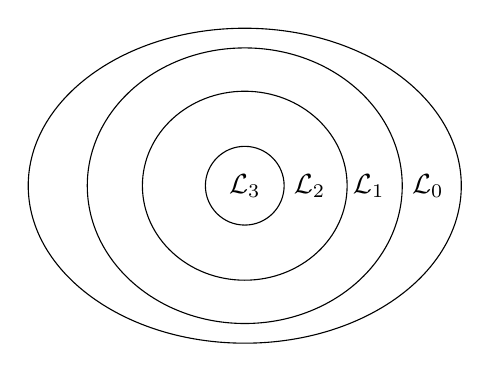
\begin{tikzpicture}
				% Sets
				\draw (0,0) ellipse (2.75cm and 2cm) node {$\mathcal{L}_3$};
				\draw (0,0) ellipse (2cm and 1.75cm) node[right=0.5cm] {$\mathcal{L}_2$};
				\draw (0,0) ellipse (1.3cm and 1.2cm) node[right=1.25cm] {$\mathcal{L}_1$};
				\draw (0,0) ellipse (0.5cm and 0.5cm) node[right=2cm] {$\mathcal{L}_0$};
			\end{tikzpicture}
		\end{center}
	\end{theorem}
\end{tcolorbox}

\textit{\textbf{Megjegyzés}}. A tartalmazásnak $\mathcal{L}_2 \subseteq \mathcal{L}_1$ része nem triviális az 1-es típusú nyelvek (nyelvtanok) kínos definíciója miatt.

A tételnek létezik az \textbf{erősebb változata}, mely valódi tartalmazást állít:
\[ \mathcal{L}_3 \subset \mathcal{L}_2 \subset \mathcal{L}_1 \subset \mathcal{L}_0. \]

Figyeljük meg, hogy a Chomsky-féle hierarchia \textbf{nyelvcsaládokra} és \textbf{nem nyelvtanokra} vonatkozik. Emiatt
\[ \mathcal{G}_3 \subseteq \mathcal{G}_2 \subsetneq \mathcal{G}_1 \subseteq \mathcal{G}_0. \]
Ha a 2-es típusú szabályoknál is kikötnénk, hogy $v \neq \emptyword$, akkor igaz lenne a tartalmazás, és akkor triviálisan igaz lenne a nyelvcsaládokra is tartalmazás.

Ha ugyanazon nemterminálishoz több szabály tartozik, akkor tömörebben is felírhatjuk a rá vonatkozó szabályokat az alábbi módon:
\[ \prodrule{S}{\emptyword \mid \texttt{a}S\texttt{b} \mid SS}, \]
ahol a ``~|~'' jelek amolyan ``\textit{vagy}'' jelentéssel bíró elválasztók. Ezt használja ki a \textbf{Backus--Naur-jelölés} (angolul \textbf{Backus--Naur-form}, röviden \textbf{BNF}), melyet a programozási nyelvek szintaxisának felírásához szoktak használni. Például ugyanez a nyelv BNF-fel felírva:
\[ \texttt{<start> ::= $\emptyword$ | a <start> b | <start> <start>}, \]
ahol a \fbox{\texttt{<}, \texttt{>}} jelek olyan \textit{metaszimbólumok}, melyekkel meg lehet címkézni az egyes nemterminálisokat. A \fbox{\texttt{::=}} felel meg a $\longrightarrow$ jelölésnek.

Egy egyszerű példa, ami néhány magyar mondat generálására képes. Az egyszerűség kedvéért feltesszük, hogy egyetlen terminális jelből áll a \texttt{macska}, \texttt{kutya}, stb. szavunk.
\begin{align*}
	&\texttt{<mondat>} & \texttt{ ::= } &\texttt{<alany> <állítmány> .} \\
	&\texttt{<alany>} & \texttt{ ::= } &\texttt{<névelő> <főnév> | <névelő> <melléknév> <főnév>} \\
	&\texttt{<névelő>} & \texttt{ ::= } &\texttt{A | Egy} \\
	&\texttt{<főnév>} & \texttt{ ::= } &\texttt{macska | kutya} \\
	&\texttt{<melléknév>} & \texttt{ ::= } &\texttt{bozontos | kerge} \\
	&\texttt{<állítmány>} & \texttt{ ::= } &\texttt{eszik | iszik | alszik}
\end{align*}

\section{Nyelvtani transzformációk}

Ahogyan korábban be lett vezetve, B szakirányon az elmélet leginkább a fordítóprogramok írásához legszükségesebb ismereteket adja át, emiatt a most következőket csak 3-as típusú nyelvtanokra, nyelvekre fogalmazzuk meg, ugyanis ezen nyelvek teszik lehetővé, hogy 

\begin{tcolorbox}
	\begin{definition}[Nyelvtani transzformáció]
		A nyelvtani transzformáció olyan eljárás, amely egy $G$ grammatikából egy másik $G'$ grammatikát készít.
	\end{definition}
\end{tcolorbox}

\begin{tcolorbox}
	\begin{definition}[Ekvivalens nyelvtani transzformáció]
		Ekvivalens nyelvtani transzformációról beszélünk, ha minden $G$ nyelvtanra és az ő $G'$ transzformáltjára igaz, hogy $L(G) = L(G')$.
	\end{definition}
\end{tcolorbox}

\subsection{Epszilon-mentesítés ($\emptyword$-mentesítés)}

A fordítóprogramok szempontjából fontos transzformációnk az ún. \textbf{\textit{$\emptyword$-mentesítés}}.

\begin{tcolorbox}
	\begin{theorem}[$\emptyword$-mentesítés]
		Minden $G = (N,T,P,S)$ \textbf{környezetfüggetlen} (2-es típusú) nyelvtanhoz megkonstruálható egy vele ekvivalens $G' = (N', T', P', S')$ \textbf{környezetfüggetlen} nyelvtan úgy, hogy $P'$-ben nincs $\prodrule{A}{\emptyword}$ alakú szabály, kivéve ha $\emptyword \in L(G)$, mert akkor $\prodrule{S'}{\emptyword} \in P'$, de ekkor $S'$ nem szerepelhez szabály jobb oldalán.
		
		Formális(abb)an:
		\[ \forall G = (N, T, P, S) \in \mathcal{G}_2 , \exists G' = (N', T', P', S') \in \mathcal{G}_2, L(G') = L(G): \]
		\begin{itemize}
			\item $\emptyword \notin L(G) \Longrightarrow$ nincs olyan szabály $P'$-ben, amely ``$\prodrule{A}{\emptyword}$'' alakú lenne,
			\item $\emptyword \in L(G) \Longrightarrow \prodrule{S'}{\emptyword} \in P'$, de ekkor $S'$ nem szerepelhet más szabály jobb oldalán.
		\end{itemize}
	\end{theorem}
\end{tcolorbox}

~\\[-2.5em]

\begin{mdframed}
	\textbf{\textit{Bizonyítás}}. A bizonyítás több lépésből áll.
	\begin{enumerate}[1.)]
		\item Határozzuk meg, hogy mely nemterminálisokból vezethető le az üres szó!
		\[ H := \left\{ A \in N \setdivbar A \genword{G}{*} \emptyword \right\}. \]
		Ehhez definiáljuk az alábbi $H_i$ halmazokat ($i \geq 1$):
		\begin{flalign*}
			H_1 & := \left\{ A \in N \setdivbar \exists \prodrule{A}{\emptyword} \in P \right\}, \\
			H_{i+1} & := H_i \cup \left\{ A \in N \setdivbar \exists \prodrule{A}{w} \in P \land w \in H_i^* \right\}.
		\end{flalign*}
		Ebből nyilvánvalóan teljesül a következő összefüggés:
		\[ H_1 \subseteq H_2 \subseteq \dots \subseteq H_i \subseteq H_{i+1}. \] 
		Mivel $\forall i \geq 1: H_i \subseteq N$ és $N$ véges halmaz, ezért egy $k \in \mathbb{N}$ indextől kezdődően biztosan azonosak lesznek a halmazok, azaz \[ \exists k \in \mathbb{N}, \forall i \in \mathbb{N} : H_k = H_{k+i}. \] Így legyen $H := H_k$.
		
		(\textit{Megjegyzés}. Ennek a részletesebb belátása az [1.] jegyzet 16. oldalán elolvasható.)
		
		Ekkor látható, hogy 
		\[  A \in N \land A \genword{G}{*} \emptyword ~~ \Longleftrightarrow ~~ A \in H. \] 
		Ennek következménye, hogy \[ \emptyword \in L(G) ~~ \Longleftrightarrow ~~ S \in H. \]
		
		\item Alakítsuk át $H$ ismeretében a grammatika szabályait a kellő alakúra.
		\begin{enumerate}
			\item $\boxed{S \notin H}$ : $\prodrule{A}{v'}\in P'$ akkor és csak akkor, ha $v' \neq \emptyword$ és $\exists \prodrule{A}{v}\in P$ úgy, hogy $v'$-t a $v$-ből úgy kapjuk meg, hogy elhagyunk nulla vagy több $H$-beli nemterminálist $v$-ből.
			\item $\boxed{S \in H}$ : A korábbi szabályhoz hozzávesszük még a következő két szabályt: 
			\[ \prodrule{S'}{\emptyword \mid S} \] ahol $S' \notin N$ és $S'$ a $G'$ nyelvtan új startszimbóluma. $\square$
		\end{enumerate}
	\end{enumerate}
\end{mdframed}

\textbf{\textit{Megjegyzés}}. A tételt ugyan 2-es típusú nyelvtanokra mondtuk ki, de 3-as típusúakra is tökéletesen működik.

\subsection{Nyelvek normálformája}

A négy nyelvtani típusból háromnak létezik ún. \textbf{normálformá}ja. Ezek a normálformák olyan alakra hozzák az adott típusú nyelvtanok szabályait, melyek egyrészt könnyebben felismerhetővé, egyértelműbbé teszik a típusát, másrészt ez az alak nagy segítségünkre válik, amikor az automatákkal is elkezdünk foglalkozni. Eme ekvivalens transzformációkra gondolhatunk úgy, mint amikor egy egyenletet rendezünk át: a végeredmény nem változik, csupán az alakja. Hasonlóan, a normálformára hozott nyelvtanok az eredeti nyelvet generálják. A tantárgy keretein belül a 2-es és 3-as típusú grammatikák normálformáját fogjuk részletesebben tárgyalni, ugyanis ezeket tudjuk hasznosítani fordítóprogramok írásánál.

Az egyes \textbf{nyelvtani típusok normálformái} a következők.

\begin{enumerate}[1. \textbf{típus.}]\bfseries
	\item Kuroda-normálforma (\textit{nem foglalkozunk vele}).
	\item \framebox{Chomsky-normálforma} és a Greibach-normálforma.
	\item \framebox{3-as típusú nyelvek normálformája.}
\end{enumerate}

Az algoritmusokat a későbbi alfejezetekben részletezzük.

\section{Automaták}

\textbf{\textit{Formális nyelvtan}}nal nyelvet szabályrendszerrel, azaz \textbf{generatív módon} adhatunk meg. Ez a megközelítés abból a szemszögből közelíti meg a nyelv szavait, hogy milyen ``törvényszerűségekkel'' lehet őket levezetni.

Azonban a gyakorlatban számtalanszor van arra szükségünk, hogy \textit{adott szóról kell eldöntenünk, hogy a nyelvnek része-e}. Ezt eldönteni pusztán a produkciós szabályokkal nem mindig könnyű eldönteni. Jó lenne, ha úgymond ``\textit{automatizálhatnánk}'' ezen kérdéskörnek a vizsgálatát. Egy olyan konstrukcióra, eszközre van szükségünk, ami egy ``\textit{igen}'' vagy ``\textit{nem}'' válasszal visszatérve eldönti, hogy a bemeneti sztring része-e a nyelvnek.

Pontosan erre a célra hozták létre az automatákat. Az \textbf{\textit{automaták}} betűről betűre megvizsgálják, hogy valid-e a nyelv szabályrendszere szerint az \textit{inputszalag}on beolvasott szó és az eredménnyel visszatérnek. Más szóval \textbf{akceptív módon} határozza meg a nyelv szavait, így beszélhetünk automata által generált nyelvről.

Mindegyik típushoz tartozik, tartoznak bizonyos típusú automaták. Róluk a megfelelő nyelvtani típusokat feldolgozó fejezetekben lesz bővebben szó. Emellett, mivel a grammatikák és az automaták annyira szorosan kapcsolódnak egymáshoz, bizonyos típusokra léteznek \textit{algoritmusok}, melyekkel \textit{grammatikát automatává lehet konvertálni és fordítva}.


\section{Zártsági tételek}

\textit{\textbf{Emlékeztető}}. \textbf{Reguláris műveletek}nek neveztük az alábbi, nyelvek felett értelmezett műveleteket: \textit{unió}, \textit{konkatenáció}, \textit{lezárás}.

Legyen $\varphi$ egy $n$-változós nyelvi művelet, azaz ha $L_1, \dots, L_n$ nyelvek, akkor $\varphi(L_1, \dots, L_n)$ is nyelv.

\begin{tcolorbox}
	\begin{definition}[Nyelvcsalád zártsága műveletre nézve]
		Az $\mathcal{L}$ nyelvcsalád zárt a $\varphi$ műveletre nézve,
		ha $L_1, \dots, L_n \in \mathcal{L}$ estén $\varphi(L_1, \dots, L_n) \in \mathcal{L}$.
	\end{definition}
\end{tcolorbox}

%\subsection{Nyelvek zártsága reguláris műveletekre}

\begin{tcolorbox}
	\begin{theorem}
		Az $\mathcal{L}_i$ $(i=0,1,2,3)$ nyelvcsaládok mindegike \textbf{zárt a reguláris műveletekre nézve}.
	\end{theorem}
\end{tcolorbox}

~\\[-2.5em]

\begin{mdframed}
	\textbf{\textit{Bizonyítás}}. Műveletenként. Az unió kivételével mindegyiknél csak $i=3$-ra látjukbe -- a mi szempontunkból ennyi bőven elég. 
	
	(\textit{Megjegyzés}. A többi nyelvcsaládra a régi jegyzet 1.9. fejezetében található részletesebb leírás (27. oldal).)
	
	Legyen $G=(N,T,P,S)$ az $L$ nyelvhez tartozó grammatika,
	$G’=(N’,T,P’,S’)$ legyen az $L’$-hez tartozó grammatika, valamint teljesüljön, hogy 
	$N \cap N’ = \emptyset$ és $G$, $G’$ azonos típusúak.
	
	\begin{enumerate}[A)]
		\item \underline{Unió}: Vezessünk be egy új startszimbólumot! Az alapkonstrukciónk:
		\[ G_\cup := \left( N \cup N’ \cup \{S_\text{új}\},T, P \cup P’ \cup \{ \prodrule{S_\text{új}}{\text{új szabály jobb oldala}} \}, S_\text{új} \right). \]
		\begin{enumerate}
			\item $\boxed{i = 0, 2, 3}$ : Legyen $S_0$ az új startszimbólum ($S_0 \notin (N \cup N’)$). Az alábbi alapkonstrukcióval fogunk dolgozni.
			\[ 	G_\cup := \left( N \cup N’ \cup \{S_0\},T, P \cup P’ \cup \{ \prodrule{S_0}{S \mid S'} \}, S_0 \right). \]
			Látható, hogy $G_\cup$ típusa megegyezik $G$ és $G’$ típusával, és $L(G) \cup L(G’) = L(G_\cup)$. Röviden, nem kell attól tartanunk, hogy az $\emptyword$-szabály elveszne.
			\item $\boxed{i = 1}$ : Ebben az esetben már elveszhet az $\emptyword$, ha $\emptyword \in (L \cup L')$. Ekkor az előbbi módon elkészített grammatikában nem teljesül a KES.
			
			Tekintsük az $L_1 := L \setminus L_\emptyword$ és $L_2 := L' \setminus L_\emptyword$ nyelveket, melyeket rendre $G_1$ és $G_2$ nyelvtanok generálnak (melyek 1-es típusúak).
			
			Készítsük el $G_\cup$-t az előbbi módon, majd vezessünk be egy $S_1$
			új kezdőszimbólumot és adjuk a szabályhalmazhoz az
			\[ \prodrule{S_1}{\emptyword \mid S_0} \]
			szabályokat (ez két szabály, tömörítve felírva).
		\end{enumerate}
		
		\newpage
		
		\item \underline{Konkatenáció}: Csak $i=3$-ra.
		
		A $P$ szabályhalmazból megkonstruálunk egy $P_1$
		szabályhalmazt úgy, hogy minden $\prodrule{A}{u}$ alakú
		szabályt felcserélünk egy $\prodrule{A}{uS'}$ alakú szabályra, a
		többi szabályt változatlanul hagyjuk.
		
		Ekkor a \[ G_C := (N \cup N', T, P_1 \cup P', S) \] grammatika 3-as típusú
		és generálja az $L(G)L(G')$ nyelvet.
		%\[ G_C := \left( N \cup N’ \cup \{S_0\},T, P \cup P’ \cup \{ \prodrule{S_0}{SS'} \}, S_0 \right). \]
		\item \underline{Lezárás}: Csak $i=3$-ra.
		
		Legyen $S_0$ új szimbólum, azaz $S_0 \notin N$.
		Definiáljuk a $P_1$ szabályhalmazt úgy, hogy minden
		$\prodrule{A}{u}$ alakú szabályt felcserélünk egy $\prodrule{A}{uS_0}$ alakú
		szabályra és ezek legyenek a $P_1$ elemei. Ekkor a
		\[ G_{*} := (N \cup \{S_0\}, T, P_1 \cup P \cup \{ \prodrule{S_0}{\emptyword \mid S} \}, S_0) \]
		grammatika generálja az $L^*$ nyelvet. $\square$
		%\[ G_* := \left( N \cup N’ \cup \{S_0\},T, P \cup P’ \cup \{ \prodrule{S_0}{SS' \mid \emptyword} \}, S_0 \right). \]
	\end{enumerate}
\end{mdframed}

\iffalse

\section{Feladatok}

\subsection{Nyelvtanok}

\begin{enumerate}
	\item Mely szavak vezethetők le az alábbi nyelvtanokból? (A kezdőszimbólumot $S$ jelöli.)
	\begin{flalign*}
		&\prodrule{S}{aA} \\
		&\prodrule{A}{c \mid bA}
	\end{flalign*}
	\begin{flalign*}
		&\prodrule{S}{\emptyword \mid aaSb}
	\end{flalign*}
	\begin{flalign*}
		\prodrule{S}&{xSy \mid A} \\
		\prodrule{xAy}&{yAx} \\
		\prodrule{xA}&{Ax} \\
		\prodrule{Ax}&{xA} \\
		\prodrule{yA}&{Ay} \\
		\prodrule{Ay}&{yA} \\
		\prodrule{A}&{\emptyword}
	\end{flalign*}
	\item Próbáljuk ki az előbbi nyelvtanokat az alábbi on-line tool-okban:
	\begin{enumerate}
		\item \hyperlink{https://mdaines.github.io/grammophone/}{https://mdaines.github.io/grammophone}
		\item \hyperlink{https://web.stanford.edu/class/archive/cs/cs103/cs103.1156/tools/cfg/}{https://web.stanford.edu/class/archive/cs/cs103/cs103.1156/tools/cfg/}
	\end{enumerate}
	\item  Készítsünk nyelvtant, mely azokat az $u \in \{ \texttt{a}, \texttt{b}\}^*$ szavakat fogadja el, melyek \texttt{a}-val kezdődnek és \texttt{b}-vel végződnek!
	\item Készítsünk nyelvtant a 4-gyel osztható bináris számok nyelvéhez!
	\item Készítsünk nyelvtant, mely $\{\texttt{a}^n\texttt{b}^n \mid n \geq 1\}$ szavait fogadja el!
	\item  Készítsünk nyelvtant ahhoz az \texttt{a}, \texttt{b} betűk feletti nyelvhez, melynek szavai ugyanannyi \texttt{a}-t és \texttt{b}-t tartalmaznak!
	\item Készítsünk nyelvtant ahhoz az \texttt{a}, \texttt{b} betűk feletti nyelvhez, melynek szavai palindrómák (megegyeznek a megfordításukkal)!
	\item Készítsünk nyelvtant a helyes zárójelezés leírására, $u \in \{\texttt{(}, \texttt{)} \}^*$
	\item  Készítsünk nyelvtant, mely $\{\texttt{a}^n\texttt{b}^n\texttt{c}^n \mid n \geq 1\}$ szavait fogadja el!
	\item $T := \{ \texttt{a}, \texttt{b}, \texttt{c}, \texttt{d} \}$. $L := \left\{ \texttt{a}^n\texttt{b}^nu \mid n \in \mathbb{N} \land \ell_\texttt{a}(u) = 1 \land u \in \left\{ \texttt{a}, \texttt{c}, \texttt{d} \right\}^* \right\}$. \\ Generáljuk $L$-et nyelvtannal! Milyen típusú ez az $L$-t generáló nyelvtan?
	\item $T := \{ \texttt{a}, \texttt{b}, \texttt{c}, \texttt{d} \}$. $L := \left\{ (\texttt{ba})^nu(\texttt{ab})^n \mid n \in \mathbb{N} \land \ell_\texttt{d}(u)=2 \land u \in \left\{  \texttt{b}, \texttt{c}, \texttt{d} \right\}^* \right\}$. \\ Generáljuk $L$-et nyelvtannal! Milyen típusú ez az $L$-t generáló nyelvtan?
	\item Adjunk nyelvtant, amely az alábbi függvénykifejezéseknek megfelelő jelsorozatokat generálja! Egy
	függvénykifejezés egy azonosítóval kezdődik és zárójelben egy vagy több argumentuma lehet. Az
	argumentumokat vessző választja el. Argumentum egy azonosító vagy függvénykifejezés lehet. Az
	azonosító betűk sorozata lehet.\\ Példák függvénykifejezésekre: $sin(f(x,y),z)$, $f(alma)$
\end{enumerate}

\subsection{Epszilon-mentesítés}

\begin{enumerate}
	\item $\emptyword$-mentesítse az alábbi grammatikát!
	\begin{flalign*}
		&\prodrule{S}{BA \mid aa} \\
		&\prodrule{A}{BB \mid aAb} \\
		&\prodrule{B}{\emptyword \mid SbA}
	\end{flalign*}
	\item $\emptyword$-mentesítse az alábbi grammatikát!
	\begin{flalign*}
		&\prodrule{S}{B \mid aa} \\
		&\prodrule{A}{SA \mid aBb} \\
		&\prodrule{B}{\emptyword \mid bBA}
	\end{flalign*}
	\item $\emptyword$-mentesítse az alábbi grammatikát! (A helyes zárójelezések nyelvét.)
	\[ \texttt{()}, \texttt{()()}, \texttt{(())}, \dots, \texttt{((())())} \in L(G) \]
	\begin{flalign*}
		&\prodrule{S}{\texttt{(} S \texttt{)} \mid SS \mid \emptyword }
	\end{flalign*}
\end{enumerate}

\fi
\chapter{Reguláris (3-as típusú) nyelvtanok}

\section{Reguláris nyelvek}

A 3-as nyelvcsalád nyelveit az alábbi módokon írhatjuk le:
\begin{itemize}
	\item 3-as típusú grammatikával,
	\item reguláris kifejezéssel,
	\item véges determinisztikus automatával (VDA),
	\item véges nemdeterminisztikus automatával (VNDA).
\end{itemize}

\textbf{\textit{Megjegyzés}}. A programozási nyelvek lexikális egységei a 3-as nyelvcsaládba tartoznak.

\begin{tcolorbox}
	\begin{proposition}
		\[ \mathcal{L}_3 = \mathcal{L}_{reg} = \mathcal{L}_{VDA} = \mathcal{L}_{VNDA}. \]
	\end{proposition}
\end{tcolorbox}

Bebizonyítható az állítás. A régi jegyzetben több tétel következményeként meggondolható. Emellett a későbbiekben be is fogjuk látni.

\begin{tcolorbox}
	\begin{definition}[Reguláris nyelvek]
		~~
		\begin{itemize}
			\item az \textbf{elemi nyelvek}: $\emptyset$, $\{\emptyword\}$, $\{a\}$ , ahol $a \in U$,
			azaz egy tetszőleges betű
			\item  azon nyelvek, melyek az elemi nyelvekből az \textbf{unió}, a \textbf{konkatenació} és a \textbf{lezárás}
			műveletek \textbf{véges számú alkalmazásával} állnak elő;
			\item  nincs más reguláris nyelv
		\end{itemize}
	\end{definition}
\end{tcolorbox}

\textbf{\textit{Példa}}. $\left\{ \{\verb*|a|\} \cup \left\{\verb*|b|\right\} \right\}^*\{\verb*|b|\} = \left\{u\verb*|b| \mid u \in \left\{a,\verb*|b|\right\}^* \right\}$.

\begin{tcolorbox}
	\begin{theorem}
		Minden $L$ reguláris nyelvhez megadható egy $G \in \mathcal{G}_3$ 3-as típusú grammatika, amelyre $L=L(G)$. $(\mathcal{L}_{reg} \subseteq \mathcal{L}_3)$
	\end{theorem}
\end{tcolorbox}

~\\[2.5em]

\begin{mdframed}
	\textbf{\textit{Bizonyítás}}. Az elemi nyelvekhez adhatunk 3-as típusú nyelvtanokat.
	\begin{itemize}
		\item $G=(\{S\},\{\verb*|a|\},\{\prodrule{S}{\texttt{a}S}\},S) ~~~ L(G)=\emptyset$. 
		\item $G=(\{S\},\{\verb*|a|\},\{\prodrule{S}{\emptyword}\},S) ~~~~~ L(G)=\{\emptyword\}$.
		\item $G=(\{S\},\{\verb*|a|\},\{\prodrule{S}{\texttt{a}}\},S) ~~~~~ L(G)=\{\texttt{a}\}$.
	\end{itemize}
	
	Korábban láttuk, hogy az $\mathcal{L}_3$ \textit{nyelvcsalád zárt a reguláris műveletekre nézve}.
	Az elemi nyelvek grammatikáiból kiindulva megkonstruálható a reguláris műveletekhez tartozó grammatika konstrukciókkal a megfelelő 3-as típusú grammatika bármely összetett reguláris nyelvhez. $\square$
\end{mdframed}

\begin{tcolorbox}
	\begin{definition}[Reguláris kifejezés]
		~
		\begin{itemize}
			\item az \textbf{elemi reguláris kifejezések}: $\emptyset$, $\emptyword$, $a$  ~~ $(a \in U)$
			\item ha $R_1$ és $R_2$ és $R$ reguláris kifejezések akkor
			\begin{enumerate}[i)]
				\item $(R_1 | R_2)$;
				\item $(R_1R_2$);
				\item $(R)^*$ is \textbf{reguláris kifejezések}.
			\end{enumerate}
			\item a \textbf{reguláris kifejezések halmaza} a legszűkebb halmaz, melyre a fenti két pont teljesül.
		\end{itemize}
	\end{definition}
\end{tcolorbox}

\textbf{\textit{Vigyázat!}} A reguláris kifejezések önmagukban nem reguláris nyelvek, azaz a reguláris kifejezés nem ugyanaz, mint a reguláris nyelv. Jelölésben az alábbi módon különböztetjük meg:
\[ L_R \text{ jelöli az } R \text{ reguláris kifejezéshez tartozó nyelvet.} \]
Az elemi nyelvekre kiterjesztve:
\begin{flalign*}
	L_\emptyset &= \emptyset, \\ L_\emptyword &= \{\emptyword\}, \\ L_a &= \{ a \} ~~~ (a \in U).
\end{flalign*}
Valamint, ha $Q$ és $R$ reguláris kifejezések, akkor:
\begin{flalign*}
	L_{(Q|R)} &= L_Q \cup L_R \\
	L_{(QR)} &= L_Q L_R \\
	L_{(R)^*} &= (L_R)^*
\end{flalign*}

A gyakorlatban sokszor nem számít ez a különbségtétel, ezért előfordulhat, hogy a jegyzetben a világosság érdekében, de a pontosság rovására ez a ``szintaktikai cukormáz'' fogja jelenteni a nyelvet.

A műveletek \textbf{prioritási sorrend}je növekvően:
\[ \text{unió } < \text{ konkatenáció } < \text{ lezárás}. \]
A zárójelek elhagyhatók a reguláris kifejezésekből a prioritásoknak megfelelően.

\section{3-as típusú nyelvtanok normálformája}

Ahogy korábban bevezettük, a nyelvtanok típusaihoz léteznek ún. \textbf{normálformák}, amelyekre gondolhatunk úgy, mint speciális formára hozott nyelvtanok, melyek ekvivalensek az eredetivel. Ezek sokszor megkönnyítik a nyelvtan vizsgálatát.

A 3-as típusú nyelvtanok normálformája az alábbi alakkal rendelkeznek.

\begin{tcolorbox}
	\begin{theorem}
		Minden 3-as típusú nyelv generálható olyan grammatikával, amelynek szabályai az alábbi alakokat ölthetik fel:
		\begin{itemize}
			\item \framebox{$\prodrule{A}{aB}$} , ahol $A,B \in N$ és $a \in T$ (egyetlen szimbólum),
			\item \framebox{$\prodrule{A}{\emptyword}$} , ahol $A \in N$.
		\end{itemize}
	\end{theorem}
\end{tcolorbox}

A normálformát a 3-as típusú nyelvtanok esetében azért szeretjük, mert \textbf{könnyű belőle automatát készíteni}. Az, hogy a normálformára hozott nyelvtanból hogyan tudunk automatát előállítani, azt a későbbiekben tárgyaljuk. Egyelőre megnézzük azt az \textbf{algoritmus}t, mellyel \textbf{normálformára hozhatunk  3-as típusú nyelvtanokat}.

~\\[-2em]

\begin{mdframed}

A \textbf{3-as normálformára hozás algoritmusa} 3 lépésből áll.

\begin{enumerate}[I.]
	\item \underline{Hosszredukció}
	
	Elhagyjuk az $\prodrule{A}{\texttt{a}_1 \dots \texttt{a}_k B}$ alakú szabályokat, ahol $k \geq 2$ és \[ \forall i  \in [1..k] : \texttt{a}_i \in T, \] valamint teljesül, hogy $A \in N$ és $B \in N \cup \{\emptyword\}$. Tehát a jobb oldalon nem szükséges, hogy nemterminális szimbólum is szerepeljen.
	
	Helyettesítsük a következő szabályokkal:
	\begin{align*}
		\prodrule{A}&{\texttt{a}_1 Z_1}, & \text{ ahol } Z_1 \notin N \to \text{ új terminális} \\
		\prodrule{Z_1}&{\texttt{a}_2 Z_2}, & \text{ ahol } Z_2 \notin (N \cup \{Z_1\}) \\
		\prodrule{Z_2}&{\texttt{a}_3 Z_3}, & \text{ ahol } Z_2 \notin (N \cup \{Z_1, Z_2\}) \\
		\cdots \\
		\prodrule{Z_{k-1}}&{\texttt{a}_k B}
	\end{align*}
	Vagyis minden szabályra új nemterminálisokat vezetünk be. Azért hívjuk hosszredukciónak ezt a lépést, mert a szabály jobb oldalának $\texttt{a}_1 \dots \texttt{a}_k \in T^k \subset T^*$ ``szeletéből'' olyan szabályokat hozunk létre, melyek már $\texttt{a}_i \in T$ ($i \in [1..k]$) terminálisokat tartalmaznak.
	
	\item \underline{Befejező szabályok átalakítása}
	
	Elhagyjuk az $\prodrule{A}{\texttt{a}}$ alakú szabályokat\footnote{Ezeket \textit{befejező szabályok}nak nevezzük.}, ahol $\texttt{a} \in T$ és $A \in B$. Ehhez felveszünk egy új nemterminálist (jelöljük $E$-vel), ami lehet közös minden befejező szabály esetén.
	
	Innen az alábbi új szabályokat felvesszük a transzformált nyelvtanunkba:
	\[ \prodrule{A}{\texttt{a}E} \text{ ~ és ~ } \prodrule{E}{\emptyword}. \]
	
	\item \underline{Láncmentesítés}
	
	Elhagyjuk az $\prodrule{A}{B}$ alakú szabályokat, ahol $A,B \in N$. Más szóval, csak nemterminális áll a szabály jobb oldalán.
	
	Első lépésben meghatározzuk minden $A \in B$ esetén a 
	\[ H(A) := \left\{ B \in N \setdivbar A \genword{G}{*} B \right\} \] halmazokat. Ehhez iteratívan definiáljuk a $H_i$ halmazokat ($i \geq 1$):
	\begin{align*}
		H_1(A) & := \{A\}, \\
		H_{i+1}(A) & := H_i (A) \cup \left\{ B \in N \setdivbar \exists C \in H_i(A) \land \prodrule{C}{B} \in P \right\}.
	\end{align*}
	Ha elkészültünk a halmazokkal, azt mondhatjuk, hogy
	\[ \exists k \in \mathbb{N}^+: H_1(A) \subseteq H_2(A) \subseteq \cdots \subseteq H_k(A) = H_{k+1}(A). \] Ekkor legyen $H(A) := H_k(A)$.
	
	Ezután felvesszük a transzformált nyelvtanba az $\prodrule{A}{X}$ szabályokat, ha
	\[ \exists B \in H(A), \prodrule{B}{X} \in P, \text{ ahol } X \in (N \cup T)^* \text{ és } X \text{ nem csak egyetlen terminális}. \]
\end{enumerate}

\end{mdframed}

\section{Véges automaták}

%\subsection{Véges determinisztikus automaták (VDA)}

\begin{tcolorbox}
	\begin{definition}
		\textbf{Véges determinisztikus automatá}nak nevezzük az \[ A = (Q, T, \delta, q_0, F) \] rendezett ötöst, ahol
		\begin{itemize}
			\item $Q$ az \textbf{állapotok halmaza} $(0 < |Q| < \infty)$,
			\item $T$ a \textbf{bemeneti szimbólumok ábécéje},
			\item $\delta : Q \times T \to Q$ leképezés az \textbf{állapot-átmeneti függvény},
			\item $q_0 \in Q$ a \textbf{kezdeti állapot},
			\item $F \subseteq Q$ az \textbf{elfogadóállapotok halmaza} (vagy \textbf{végállapotok halmaza})
		\end{itemize}
	\end{definition}
\end{tcolorbox}

\textbf{\textit{Megjegyzés}}. Fontos, hogy \textit{véges determinisztikus automata} esetén a $\delta$ függévny értelmezett minden $(q,a) \in Q \times T$ párra, azaz
\[ \forall (q,a) \in Q \times T, \exists! p \in Q : \delta(q, a) = p. \]

Ha ez nem teljesül, azaz egy $(q,a)\in Q \times T$ párhoz több $p\in Q$ állapot is tartozhat, akkor \textit{véges \textbf{nem}determinisztikus automatá}ról beszélünk (\textit{VNDA} vagy \textit{NDA}).

\begin{tcolorbox}
	\begin{definition}
		\textbf{Véges nemdeterminisztikus automatá}nak nevezzük az \[ A = (Q, T, \delta, Q_0, F) \] rendezett ötöst, ahol
		\begin{itemize}
			\item $Q$ az \textbf{állapotok halmaza} $(0 < |Q| < \infty)$,
			\item $T$ a \textbf{bemeneti szimbólumok ábécéje},
			\item $\delta : Q \times T \to \mathcal{P}(Q)$ leképezés az \textbf{állapot-átmeneti függvény},
			\item $Q_0 \subseteq Q$ a \textbf{kezdőállapotok halmaza},
			\item $F \subseteq Q$ az \textbf{elfogadóállapotok halmaza} (vagy \textbf{végállapotok halmaza})
		\end{itemize}
	\end{definition}
\end{tcolorbox}

Felhívjuk a figyelmet arra a pár apró, ugyan lényekes különbségre, ami ebben a definícióban található.
\begin{itemize}
	\item Egyrészt, a egyetlen kezdőállapot helyett kezdőállapotok halmazáról beszélünk.
	\item Az állapot-átmenetek függvénye a $Q$ hatványhalmazába képez (amit $\mathcal{P}(Q)$-val jelölünk). Ez engedi meg, hogy egy adott $(q,a)$ párhoz több állapotot is hozzárendelhessünk.
\end{itemize}
A VNDA a VDA általánosításának tekinthető.

Hogy kövessük az eddig bevezetett konvenciókat, az állapot-átmeneteket is felírhatjuk olyan szintaxissal, amellyel a produkciós szabályokat írtuk fel.
\[ \delta(q,a) = p ~~~ \Longleftrightarrow ~~~ \prodrule{qa}{p}. \]

Az automaták témakörében is értelmezzük a \textit{mondatform}ának megfeleltethető fogalmat, amit \textbf{konfiguráció}nak nevezünk.

\begin{tcolorbox}
	\begin{definition}[Konfiguráció]
		A $v \in QT^*$ egy konfigurációja egy VDA-nak, ha az aktuális állapotot és az inoput hátralévő részét tartalmazza, azaz $v = qu$.
	\end{definition}
\end{tcolorbox}

Hasonlóan, a \textit{közvetlen és közvetett levezetés}nek is létezik megfelelője. Ezeket \textbf{közvetlen}, ill. \textbf{közvetett redukció}nak nevezzük. A redukció név arra utal, hogy az inputszalagról beolvasott szöveg hossza egyre csökken.

\begin{tcolorbox}
	\begin{definition}[Közvetlen redukció]
		Legyen $A = (Q,T,\delta,q_0,F)$ egy VDA és legyenek $u,v \in Q^*$ konfigurációk.
		
		Azt mondjuk, hogy az $A$ automata az $u$ konfigurációt a $v$ konfigurációra \textbf{redukálja közvetlenül}, ha
		\[ \exists \delta(q,a)=p \text{ szabály} \land \exists w \in T^* : u = qaw \land v = pw. \]
		Jele: $u\genword{A}{}v$.
	\end{definition}
\end{tcolorbox}

Alternatív módon: van olyan $\prodrule{qa}{p}$ szabály és van olyan $w \in T^*$ szó, amelyre \[u=\textbf{qa}w \land v = \textbf{p}w.\] A vastag kijelölés nem azt jelenti, hogy vektorok lennének, hanem hogy szemléletesebben kiemeljem a ``csere'' helyét.

A \textbf{közvetett redukció}t gyakran csak egyszerűen \textbf{redukció}nak nevezzük.

\begin{tcolorbox}
	\begin{definition}[Redukció vagy közvetett redukció]
		Az $A = (Q,T,\delta,q_0,F)$ véges automata az $u \in QT^*$ konfigurációt a $v \in QT^*$ konfigurációra \textbf{redukálja}, ha
		\begin{itemize}
			\item ha $u = v$, vagy
			\item ha $u \neq v$, akkor $\exists z \in QT^* : u \genword{A}{*} z \land z \genword{A}{} v$.
		\end{itemize}
		Jele: $u\genword{A}{*}v$.
	\end{definition}
\end{tcolorbox}

Ahogy a grammatikáknál is, itt is értelmezzük az automata által elfogadott nyelvet. Figyeljük meg a szóhasználatot: az automata továbbra sem generálja, hanem elfogadja a szavakat (akceptív módon közelíti meg a szóproblémát).

\begin{tcolorbox}
	\begin{definition}[Automata által elfogadott nyelv]
		Az $A = (Q,T,\delta,q_0,F)$ véges automata által elfogadott nyelv alatt az
		\[ L(A) := \left\{ u \in T^* \setdivbar q_0 u \genword{A}{*} p \land p \in F \right\} \]
		szavak halmazát értjük.
	\end{definition}
\end{tcolorbox}

A definíció azt jelenti, hogy az automata a kezdőállapotból ($q_0$-ból) indulva végig olvasva az inputot
elfogadóállapotba jut (azaz $p \in F$).

\subsection{3-as típusú nyelvek kapcsolata a véges automatákkal}

\begin{tcolorbox}
	\begin{theorem}
		Minden 3-as típusú $L$ nyelvhez megadható egy véges nemdeterminisztikus automata, és fordítva; minden nemdeterminisztikus automata 3-as típusú nyelvet ismer fel.
		\[ \mathcal{L}_3 \subseteq \mathcal{L}_{VNDA} \text{ ~ és ~ } \mathcal{L}_{VNDA} \subseteq \mathcal{L}_3 \]
	\end{theorem}
\end{tcolorbox}

\textbf{\textit{Bizonyítás}}. // Kidolgozni.

\begin{tcolorbox}
	\begin{theorem}
		Minden $A=(Q,T,\delta,Q_0,F)$ nemdeterminisztikus automatához megadható egy
		$A'=(Q',T,\delta',q_0',F')$ véges determinisztikus automata, hogy az általuk generált nyelvek ekvivalensek, azaz \[  \forall A=(Q,T,\delta,Q_0,F) , \exists A'=(Q',T,\delta',q_0',F') : L(A')=L(A). \]
		\[ \mathcal{L}_{VNDA} \subseteq \mathcal{L}_{VDA} \]
	\end{theorem}
\end{tcolorbox}

\textbf{\textit{Bizonyítás}}. // Kidolgozni.

\begin{tcolorbox}
	\begin{theorem}[Kleene tétele]
		\[ \mathcal{L}_3 = \mathcal{L}_{reg} \]
	\end{theorem}
\end{tcolorbox}

\textbf{\textit{Bizonyítás}}. // Kidolgozni.

\subsection{Minimális véges determinisztikus automata}

\begin{tcolorbox}
	\begin{definition}[Minimális véges determinisztikus automata]
		Az $A$ véges determinisztikus automata \textbf{minimális állapotszámú},
		ha nincs olyan $A'$ véges determinisztikus automata, amely
		ugyanazt a nyelvet ismeri fel, mint $A$, de $A'$ állapotainak száma
		kisebb, mint $A$ állapotainak száma.
		\[ \exists A'=(Q', T, \delta', q_0', F') \text{ véges det. autom.} : L(A') = L(A') \land |Q'| < |Q| \]
	\end{definition}
\end{tcolorbox}

\begin{tcolorbox}
	\begin{theorem}
		Az $L$ reguláris nyelvet felismerő \textbf{minimális} véges determinisztikus automata az izomorfizmus erejéig \textbf{egyértelmű}.
	\end{theorem}
\end{tcolorbox}

\textbf{\textit{Bizonyítás}}. // Kidolgozni.

\begin{tcolorbox}
	\begin{definition}[Elérhető állapot]
		Az $A = (Q, T, \delta,q_0, F)$ véges determinisztikus automata
		$q$ \textbf{állapot}át \textbf{elérhető}nek mondjuk,
		ha \[ \exists u \in T^* : q_0 u \genword{A}{*} q. \]
	\end{definition}
\end{tcolorbox}

\begin{tcolorbox}
	\begin{definition}[Összefüggő VDA]
		Az $A = (Q, T, \delta,q_0, F)$ véges determinisztikus automatát
		\textbf{összefüggő}nek mondjuk, ha minden állapota elérhető a
		kezdőállapotból.
	\end{definition}
\end{tcolorbox}

\begin{tcolorbox}
	\begin{definition}[Ekvivalens állapotok]
		Legyen $A = (Q, T, \delta,q_0, F)$ egy VDA és $q, p \in Q$ állapotok.
		Ekkor $q$ és $p$ \textbf{ekvivalens állapotok},
		ha
		\begin{gather*}
			\forall u \in T^* \text{ szóra teljesül, hogy } qu \genword{A}{*} r \text{ és } pu \genword{A}{*} r' \text{ esetén } \\
			r \in F \text{ akkor és csak akkor, ha } r' \in F.
		\end{gather*}
		Jele: \framebox{$q \sim p$} .
	\end{definition}
\end{tcolorbox}

\begin{tcolorbox}
	\begin{proposition}
		Ha $q$ és $p$ ekvivalens, akkor $\prodrule{qa}{s}$ és $\prodrule{pa}{t}$
		esetén $s$ és $t$ is ekvivalens állapotok $\forall a \in T$ betűre.
	\end{proposition}
\end{tcolorbox}

\begin{tcolorbox}
	\begin{definition}[$i$-ekvivalens állapotok]
		Legyen $A = (Q, T, \delta,q_0, F)$ egy VDA és $q, p \in Q$ állapotok.
		Az mondjuk, hogy $q$ és $p$ \textbf{$i$-ekvivalens állapotok}, ha 
		\begin{gather*}
			\forall u \in T^* \text{ szóra, ahol } \ell(u) \leq i \text{ teljesül, hogy  } \\
			qu \genword{A}{*} r \text{ és } pu \genword{A}{*} r' \text{ esetén } r \in F\text{ akkor és csak akkor, ha } r' \in F.
		\end{gather*}
		Jele: \framebox{$q \sim ^i p$} vagy \framebox{$q \partition{i} p$} .
	\end{definition}
\end{tcolorbox}

\begin{tcolorbox}
	\begin{lemma}
		\[ q \partition{i+1} p ~ \Longleftrightarrow ~ \forall a \in T , \prodrule{qa}{s} \land \prodrule{pa}{t} : s \partition{i} t. \]
	\end{lemma}
\end{tcolorbox}

Szavakban: legfeljebb $i$ hosszú szavak esetén a két állapot nem megkülönböztethető.

\iffalse

\section{Feladatok}

\subsection{Reguláris kifejezések}

\begin{enumerate}
	\item Mely alábbi szavakra illeszkednek az alábbi reguláris kifejezések? \\
	Reguláris kifejezések: ””, a, ab, a|b, a*, a|b*, ab*, a*b, a*b, a*b*, a*|b*, (ab)* \\
	Szavak: $\emptyword$, a, b, aa, ab, ba, aaa, aab, aba, abb, baa, bab, bba, bbb, aaaaaa, bbbbb, ababab, babab
	\item  Mely szavakra illeszkedik az \texttt{a?} reguláris kifejezés? Írjuk fel a standard műveletek segítségével!
	\item Mely szavakra illeszkedik az \texttt{a+} reguláris kifejezés? Írjuk fel a standard műveletek segítségével!
	\item Mely szavakra illeszkedik az \texttt{[a-d]} reguláris kifejezés? Írjuk fel a standard műveletek segítségével!
	\item Mely szavakra illeszkedik az \verb|[^a-z]| reguláris kifejezés? Kezdjük el felírni a standard műveletek
	segítségével!
	\item Adjon meg reguláris kifejezést a következő számformátumokhoz!
	\begin{enumerate}
		\item Decimális egész szám (legalább egy számjegy \texttt{0-9}-ig)
		\item Olyan decimáis egész szám, amely több számjegy esetén nem kezdődhet nullával
		\item Előjeles decimális egész szám (opcionális \texttt{+} vagy \texttt{–} az elején)
		\item Decimális törtszám (tizedespont előtt legalább egy számjegy)
	\end{enumerate}
	\item Készítsen reguláris kifejezést a helyes \texttt{hh:mm} óraformátum ellenőrzésére, ahol a \texttt{hh} a \texttt{00..23}, míg az \texttt{mm} a \texttt{00..59} értékeket veheti fel!
	\item Adjon meg reguláris kifejezést a következő azonosítókhoz! (Betűk alatt az angol ábécé kis- és nagybetűit, számjegyek alatt a decimális számjegyeket értjük.)
	\begin{enumerate}
		\item Betűvel kezdődik, számjeggyel, betűvel vagy \texttt{\_} jellel folytatódik
		\item Szigorítás: az utolsó karakter nem lehet \texttt{\_}
		\item További szigorítás: nem lehet egymás mellett két \texttt{\_}
	\end{enumerate}
	\item Adjon meg reguláris kifejezést a következő, trükkösebb azonosítókhoz!
	\begin{enumerate}
		\item Az első fele csak betűket illetve \texttt{\_} jelet tartalmazhat, második fele pedig csak számjegyeket
		\item Szigorítás: Ha a betűkből álló rész legelső és legutolsó karaktere is \texttt{\_} akkor közte csak nagybetűk
		szerepelhetnek, egyébként pedig csak kisbetűk
		\item További szigorítás: Ha a számjegyekből álló rész első számjegye páros akkor utána még páros darab számjegy következhet, ha az első páratlan akkor pedig még páratlan darab.
	\end{enumerate}
	\item Adjon meg reguláris kifejezést a következő, furcsa azonosítókhoz! Az azonosító csak az \texttt{a}, \texttt{b}, \texttt{c} betűket tartalmazhatja (akár többször is, de nem kötelező mindegyiket), viszont a betűknek be kell tartania az \texttt{abc} sorrendet, azaz egy \texttt{a} előtt soha nem szerepelhet \texttt{b} vagy \texttt{c}, illetve egy \texttt{b} előtt nem szerepelhet \texttt{c}. \\
	Helyes: \texttt{abc}, \texttt{aaabcc}, \texttt{ac}, \texttt{c} \\
	Helytelen: \texttt{bac}, \texttt{abcb}, \texttt{bcbc}
	\item Adjon meg reguláris kifejezést egysoros megjegyzésekhez, amely \texttt{//}-től a sor végéig tartanak!
	\item Adjon meg reguláris kifejezést többsoros megjegyzésekhez, amelyek \texttt{/*}-tól \texttt{*/}-ig tartanak! \\
	Helyes: \texttt{/**/}, \verb*|/*ab”+!%/=.*/|, \verb*|/******/|, \verb*|/*//////*/| \\
	Helytelen: \verb*|abc|, \verb*|*|, \verb*|/|, \verb|/*, */|, \verb*|/*/|, \verb*|/*abc*/abc*/|
	\item Adjon meg reguláris kifejezést sztring leírására! A sztringek idézőjellel kezdődnek és végződnek, a belsejükben tetszőleges karakterek szerepelhetnel az alábbiak betartásával:
	\begin{enumerate}
		\item Idézőjel nem állhat belül, kizárólag \verb*|text| után.
		\item \verb*|\\| és \verb*|\”| szabályosak a sztring belsejében, más kombinációban \verb*|text| nem szerepelhet.
		\item Példák: \verb*|"alma"|, \verb|"a \" egy idézőjel a sztringben”|, \\ \verb|"a \\ egy backslash a sztringben"|
		\item Adjon meg reguláris kifejezést fehér szóközök (\textit{space}, \textit{tab} vagy \textit{sorvége}) nem üres sorozataira!
	\end{enumerate}
\end{enumerate}

\subsection{3-as típusú nyelvtanok normálformája}

Mai órán hasznos eszköz: \hyperlink{http://madebyevan.com/fsm/}{http://madebyevan.com/fsm/}
\begin{enumerate}
	\item tartalom...
\end{enumerate}

\subsection{Véges (nem) determinisztikus automaták}

%Mai órán hasznos eszköz: \hyperlink{http://madebyevan.com/fsm/}{http://madebyevan.com/fsm/}
\begin{enumerate}
	\item tartalom...
\end{enumerate}

\fi

\chapter{A 2-es és 3-as nyelvcsalád viszonya}

A következő tételek szükséges feltételeket fogalmaznak meg a 3-as típusú
nyelvekre. Vannak nyelvek, amelyek bizonyíthatóan nem teljesítik a feltételeket,
de 2-es típusú grammatikával generálhatók.

\section{Szükséges feltétel 3-as típusú nyelvekre}

\begin{tcolorbox}
	\begin{lemma}[Kis Bar-Hillel lemma]
		$\forall L \in \mathcal{L}_3$ nyelvhez $\exists n \in \mathbb{N}^+$ \textbf{nyelvfüggő
		konstans}, hogy $\forall u \in L$, ahol $\ell(u) \geq n$ szó esetén van
		u-nak olyan $u = xyz$ felbontása, amelyre
		\begin{itemize}
			\item $\ell(xy) \leq n$,
			\item $y \neq \emptyword$,
			\item $\forall i \in \mathbb{N} : xy^iz \in L$.
		\end{itemize}
	\end{lemma}
\end{tcolorbox}

\textbf{\textit{Bizonyítás}}. // Kidolgozni.

\section{Szükséges és elégséges feltétel 3-as típusú nyelvekre}

\begin{tcolorbox}
	\begin{definition}[Maradéknyelv]
		Legyen $L$ egy $T$ ábácé felett értelmezett nyelv $(L \subseteq T^*)$.
		Az $L$ nyelv egy $p \in T^*$ \textbf{szóra értelmezett maradéknyelve} a következő:
		\[ L_p := \{ u \in T^* \mid pu \in L \} . \]
	\end{definition}
\end{tcolorbox}

\begin{tcolorbox}
	\begin{theorem}[Myhill--Nerode-tétel]
		Egy $L$ nyelv akkor és csak akkor 3-as típusú, ha a véges számú maradéknyelve van, azaz
		\[ L \in \mathcal{L}_3 ~ \Longleftrightarrow ~ \left| \left\{ L_p \setdivbar p \in T^* \right\} \right| < \infty . \]
	\end{theorem}
\end{tcolorbox}

\textbf{\textit{Megjegyzés}}. A szavakon egy osztályozást végzünk az
adott nyelvtől függően.

\textbf{\textit{Bizonyítás}}. // Kidolgozni.

%\section{Feladatok}
\chapter{Környezetfüggetlen (2-es típusú) nyelvtanok}

\section{A szóprobléma kérdése}

A \textit{formális nyelvek} témakörében az egyik központi kérdésünk, hogy adott $G$ grammatika és adott $u \in T^*$ szó estén teljesül-e, hogy $u \in L(G)$. Vagyis, hogy a $G$ nyelvtan által generált nyelvben benne van-e az $u$ szó. Szerencsére, a 2-es típusú nyelvtanok esetében vannak eszközeink ezen kérdésnek eldöntésére.

Ez az úgynevezett \textbf{szintaxisfa}, vagy \textbf{levezetési fa}. Az elnevezés több értelmet nyer, ha felidézzük a Backus--Naur-jelölést.

\begin{tcolorbox}
	\begin{definition}[Szintaxisfa]
		Legyen $G = (N,T,P,S) \in \mathcal{G}_2$ grammatika.
		A $t$ nemüres fát \textbf{$G$ feletti levezetési (szintaxis) fának}
		nevezzük, ha
		\begin{itemize}
			\item pontjai $T \cup N \cup \{\emptyword\}$ elemeivel vannak címkézve;
			\item belső pontjai $N$ elemeivel vannak címkézve;
			\item ha egy belső pont címkéje $A$, a közvetlen
			leszármazottjainak címkéi pedig balról jobbra olvasva
			$X_1, X_2, \dots, X_k$, akkor $A \longrightarrow X_1X_2\dots X_k \in P$.
			\item az $\emptyword$-nal címkézett pontoknak nincs testvére.
		\end{itemize}
	\end{definition}
\end{tcolorbox}

\begin{tcolorbox}
	\begin{theorem}
		Ha adott $G$ grammatika esetén $u \in L(G)$ akkor és csak
		akkor, ha $u$-hoz \textbf{megadható egy szintaxisfa}.
	\end{theorem}
\end{tcolorbox}

\textbf{\textit{Megjegyzés}}. Az $u$-hoz tartozó szintaxisfa gyökere $S$ és
a leveleit \textit{balról jobbra} összeolvasva az $u$ szót kapjuk.

\begin{tcolorbox}
	\begin{proposition}
		Minden szintaxisfához megadható egy levezetés és fordítva.
	\end{proposition}
\end{tcolorbox}

\begin{tcolorbox}
	\begin{definition}[Egyértelmű nyelvtan]
		Egy $G \in \mathcal{G}_2$ nyelvtan \textbf{egyértelmű}, ha minden $u \in L(G)$ szóhoz egyetlen szintaxisfa tartozik.
	\end{definition}
\end{tcolorbox}

%Megelőlegezzük, hogy \textbf{a szóprobléma eldönthető az összes környezetfüggetlen nyelvtan által generált nyelvre}. Ennek eldöntésére szintén egy új automatát vezetünk be, az ún. \textbf{veremautomatá}kat. Róluk pár alfejezettek később lesz bővebben szó.

\section{2-es típusú nyelvtanok normálformája}

A Chomsky-hierarchia bevezetésénél kimondtuk az \textbf{$\emptyword$-mentesítés} tételét, amit 2-es és 3-as típusú nyelvtanokon elvégezhető transzformáció. 

\begin{tcolorbox}
	\begin{definition}[Chomsky-normálforma]
		Egy $G=(N,T,P,S) \in \mathcal{G}_2$ %környezetfüggetlen
		nyelvtant \textbf{Chomsky-normálformájú}nak
		mondunk, ha szabályai
		\begin{itemize}
			\item \framebox{$\prodrule{A}{a}$} , ahol $A \in N$ és $a \in T$ vagy
			\item \framebox{$\prodrule{A}{BC}$} alakúak, ahol $A, B, C \in N$.
			\item \framebox{$\prodrule{S}{\emptyword}$} , de ekkor $S$ nem fordul elő egyetlen
			szabály jobboldalán sem.
		\end{itemize}
	\end{definition}
\end{tcolorbox}

\begin{tcolorbox}
	\begin{theorem}	
		Minden \textbf{környezetfüggetlen} grammatikához
		megkonstruálható egy vele ekvivalens \textbf{Chomsky
		normálformájú} grammatika.
	\end{theorem}
\end{tcolorbox}

\textbf{\textit{Megjegyzések}}.
\begin{itemize}
	\item A 2-es típusú grammatikák Chomsky normálformára hozásának algoritmusa nem a
	tananyag része.\footnote{A jegyzet írása idején így szólt a tanterv (2023/2024/2. félév).}
	\item Chomsky normálformájú grammatikákhoz megadható olyan elemző program,
	amely $O(n^3)$ időben eldönti a szóproblémát (\textit{Cocke--Younger--Kasami-algoritmus}).
	\item Bizonyos állítások bizonyítását elég elvégezni a normálformájú grammatikákra.
\end{itemize}

A korábban 3-as típusú nyelvtanokra megfogalmazott \textit{kis Bar-Hillel lemmá}t megfogalmazzuk környezetfüggetlen nyelvekre is.

\begin{tcolorbox}
	\begin{lemma}[Nagy Bar-Hillel lemma]
		$\forall L \in \mathcal{L}_2$ nyelvhez $\exists p, q \in \mathbb{N}$ \textbf{nyelvfüggő
		konstans}, hogy $\forall u \in L$, ahol $\ell(u) \geq p$ szó esetén van
		$u$-nak olyan $u = vxwyz$ felbontása $(v, x, w, y, z \in T^*)$, amelyre
		\begin{itemize}
			\item $\ell(xwy) \leq q$,
			\item $xy \neq \emptyword$,
			\item $\forall i \in \mathbb{N} : vx^iwy^iz \in L$.
		\end{itemize}
	\end{lemma}
\end{tcolorbox}

\textbf{\textit{Megjegyzések}}.
\begin{itemize}
	\item A lemma \textbf{szükséges feltétel} környezetfüggetlen nyelvekre.
	\item A lemmát nem bizonyítjuk, de a bizonyításhoz szükséges, hogy a
	2-es típusú nyelvekhez létezik Chomsky-normálformájú grammatika.
\end{itemize}

\textbf{\textit{Következmény}}. Van olyan nyelv, amely nem környezetfüggetlen. Például
\[ L := \{ \texttt{a}^n\texttt{b}^n\texttt{c}^n \mid n > 0 \} \notin \mathcal{L}_2. \]
Tegyük fel indirekt, hogy $\exists p, q$ a Bar-Hillel lemmának megfelelő konstansok. Legyen $k > p$ és $k > q$ is. Ekkor $u = \texttt{a}^n\texttt{b}^n\texttt{c}^n$ és $\ell(u) > p$.

A lemma szerint az $u$ szó $vxwyz$ alakban felbontható kell legyen, úgy, hogy $\ell(xwy) \leq q <k$ és $x$ és $y$ párhuzamosan beiterálható. De ekkor $xy$-ban nem lehet mindhárom betűből, így $vwz$ nem
lehet eleme $L$-nek, ami ellentmondás.

\section{Nyelvtan redukálása}

A grammatikák transzformálása közben keletkezhetnek olyan szabályok, amelyek egyetlen szó levezetésében sem használhatóak.

A grammatikában lehetnek olyan nemterminálisok, amelyekből

\begin{enumerate}
	\item nem lehet csupa nem terminálisból álló sorozatot
	előállítani (\textit{zsákutcák});
	\item nem érhetők el a kezdőszimbólumból.
\end{enumerate}

\begin{tcolorbox}
	\begin{definition}[Aktív nemterminálisok]	
		\textbf{Aktív} nemterminálisok halmaza egy adott $G=(N,T,P,S)\in \mathcal{G}_2$ grammatika esetén:
		\[ A := \left\{ X \in N \setdivbar X \genword{G}{*} u \land u \in T^* \right\}. \] 
	\end{definition}
\end{tcolorbox}

Inaktív (\textbf{zsákutca}) nemterminálisok: $\boxed{N \setminus A}$ .

\begin{tcolorbox}
	\begin{definition}[Elérhető nemterminálisok]	
		\textbf{Elérhető} nemterminálisok halmaza egy adott $G=(N,T,P,S)\in \mathcal{G}_2$ grammatika esetén:
		\[ R := \left\{ X \in N \setdivbar S \genword{G}{*} uXw \land u, w \in (T \cup N)^* \right\}. \] 
	\end{definition}
\end{tcolorbox}

Nem elérhető nemterminálisok: $\boxed{N \setminus R}$ .

\begin{tcolorbox}
	\begin{definition}[Hasznos nemterminálisok]	
		Egy nemterminálist \textbf{hasznos}nak mondunk, ha \textbf{aktív és elérhető}:
		\[ X \in (A \cap R) \subseteq N. \]
	\end{definition}
\end{tcolorbox}

\begin{tcolorbox}
	\begin{definition}[Redukált nyelvtan]	
		Egy környezetfüggetlen grammatika
		\textbf{redukált}, ha minden nemterminálisa \textbf{hasznos}, azaz
		a grammatika \textbf{zsákutcamentes és összefüggő}.
	\end{definition}
\end{tcolorbox}

\begin{tcolorbox}
	\begin{theorem}
		Minden $G \in \mathcal{G}_2$ nyelvtanhoz
		megkonstruálható egy vele ekvivalens \textbf{redukált grammatika}.
	\end{theorem}
\end{tcolorbox}

\textbf{\textit{Bizonyítás}}. // Kidolgozni.

\begin{enumerate}
	\item Zsákutcák meghatározása és minden olyan szabály
	elhagyása, amiben inaktív nemterminálisok szerepelnek.
	\item Az $S$-ből nem elérhető nemterminálisokhoz tartozó
	szabályok elhagyása, azaz a grammatika összefüggővé
	tétele.
\end{enumerate}

\section{Veremautomaták}

Elöljáróban elárultuk, hogy a szóprobléma eldönthető az összes környezetfüggetlen nyelvtan által generált nyelvre. Íme az erre vonatkozó tétel és bizonyítása.

\begin{tcolorbox}
	\begin{theorem}[Szóprobléma eldöntése]
		Minden $G=(N,T,P,S)\in \mathcal{G}_2$ grammatika esetében eldönthető, hogy
		egy tetszőleges $u \in T^*$ szó benne van-e a $G$
		grammatika által generált nyelvben vagy sem.
	\end{theorem}
\end{tcolorbox}

\textbf{\textit{Bizonyítás}}. // Kidolgozni.

A szóprobléma eldönthető a környezetfüggetlen grammatikákhoz párosuló \textbf{veremautomatá}kkal, melyet az alábbi módon definiálunk.

\begin{tcolorbox}
	\begin{definition}[Veremautomata] \textbf{Veremautomatá}nak nevezzük az
		\[ A = (Z, Q, T, \delta, z_0, q_0, F) \]
		rendezett hetest, ahol
		\begin{itemize}
			\item $Z$ a verem szimbólumainak ábécéje,
			\item $Q$ az állapotok halmaza $(0 < |Q| < \infty)$,
			\item $T$ a bemeneti szimbólumok ábécéje,
			\item $\delta : Z \times Q \times (T \cup \{\emptyword\}) \to \mathcal{P}(Z^* \times Q)$ leképezés az állapotátmeneti függvény, ahol $\delta$ véges részhalmazokba képez,
			\item $z_0 \in Z$ a kezdő veremszimbólum,
			\item $q_0 \in Q$ a kezdőállapot
			\item $F \subseteq Q$ az elfogadóállapotok halmaza.
		\end{itemize}
	\end{definition}
\end{tcolorbox}

Egy lépésben mindig kell egy jelet olvasni a verem tetejéről és csak egy jelet lehet
elérni. Az input szalagról is egy jelet lehet olvasni, de nem kötelező.

Megváltoztatható az automata aktuális állapota, illetve a verem teteje. Egy lépésben
egy egész sorozatot is beírhatunk a verembe.

\textbf{\textit{Példák}}.
\begin{itemize}
	\item \framebox{$\delta(\#,q,a) = \{(\#a,q)\}$} \\ \textit{Jelentése}: Ha \# van a verem tetején és $a$ betű jön az inputon, akkor \textbf{tegyük be} $a$-t a verembe. Ne változtassunk az állapoton.
	
	\item \framebox{$\delta(\#,q,a) = \{(\emptyword,q)\}$} \\ \textit{Jelentése}: Ha \# van a verem tetején és $a$ betű jön az inputon, akkor \textbf{töröljük} \#-t a veremből. Ne változtassunk az állapoton.
	
	\item \framebox{$\delta(\#,q,a) = \{(\#,r)\}$} \\ \textit{Jelentése}: Ha \# van a verem tetején és $a$ betű jön az inputon, akkor \textbf{ne változtassuk a verem tartalmát}. Viszont váltsunk állapotot. 
	
	\item \framebox{$\delta(\#,q,\emptyword) = \{(\#bb,q)\}$} \\ \textit{Jelentése}: Ha \# van a verem tetején és nem olvasunk az inputról, akkor \textbf{tegyünk a verembe} két $b$ betűt és váltsunk állapotot is.
\end{itemize}

Ahogyan azt a véges automatáknál is tapasztalhattuk, létezik az állapotátmeneteknek egy alternatív jelölése, mely követi azt a konvenciót, ahogyan a nyelvtani szabályokat írjuk fel.

\begin{itemize}
	\item Ha $\delta(z,q,a) = \{(w_1,r_1),\dots,(w_k,r_k)\}$ $(k \in \mathbb{N}^+)$ , akkor ezt a leképezést a következő szabályhalmazzal is jelölhetjük:
	\[ \prodrule{zqa}{w_i r_i} ~~~~ i \in [1 \dotdot k]. \]
	\item Ha $\delta(z,q,\emptyword) = \{(w_1,r_1),\dots, (w_k,r_k)\}$ $(k \in \mathbb{N}^+)$, akkor ezt a leképezést a következő szabályhalmazzal is jelölhetjük:
	\[ \prodrule{zq}{w_i r_i} ~~~~ i \in [1 \dotdot k]. \]
\end{itemize}

Tehát a szabályok bal oldala $ZQT$ vagy $ZQ$ alakú és a jobboldala $Z^*Q$ alakú.

Ahogyan a véges automatáknál, itt is értelmezzük a \textbf{konfiguráció} fogalmát -- természetesen a megfelelő módosításokkal.

\begin{tcolorbox}
	\begin{definition}[Konfiguráció]
		Legyen $A = (Z, Q, T, \delta, z_0, q_0, F)$ egy veremautomata és
		legyen $\alpha \in Z^*QT^*$.
		Azt mondjuk $\alpha$ az $A$ veremautomata egy \textbf{konfigurációja}.
	\end{definition}
\end{tcolorbox}

Szavakban: a konfiguráció a veremautomata egy pillanatnyi állapotát írja le.

Hasonlóan, a redukciót fogalmát is értelmezzük. Ahogy azt a véges automatáknál is tapasztalhattuk, a ``sima'' redukció magába foglalja a közvetett redukciót, így a kettőt nem szoktuk megkülönböztetni.

\begin{tcolorbox}
	\begin{definition}[Közvetlen redukció]
		Legyen $A = (Z, Q, T, \delta, z_0, q_0, F)$ egy veremautomata és
		legyen $\alpha, \beta \in Z^*QT^*$ konfigurációk.
		
		Azt mondjuk, hogy az A veremautomata az $\alpha$ konfigurációt
		a $\beta$ konfigurációra \textbf{redukálja közvetlenül}, ha
		\[ \exists z \in Z, p, q \in Q, a \in T\cup\{\emptyword\}, r,u \in Z^*, w \in T^*, \text{ hogy } \]
		\begin{itemize}
			\item \framebox{$\prodrule{zqa}{up}$} egy szabály $\delta$-ban,
			\item $\alpha = r\textbf{zqa}w$ és $\beta = r\textbf{up}w$.
		\end{itemize}
		~
		
		Jele: \framebox{$\alpha \genword{A}{} \beta$} .
	\end{definition}
\end{tcolorbox}

A vastag betűk továbbra is arra szolgálnak, hogy szemléletesebbé váljon a helyettesítés és nem vektorokat jelentenek.

\begin{tcolorbox}
	\begin{definition}[Redukció]
		Legyen $A = (Z, Q, T, \delta, z_0, q_0, F)$ egy veremautomata és
		legyenek $\alpha, \beta \in Z^*QT^*$ konfigurációk.
		
		Azt mondjuk, hogy az A veremautomata az $\alpha$ konfigurációt
		a $\beta$ konfigurációra \textbf{redukálja közvetetten}, 
		\begin{itemize}
			\item ha vagy $\alpha = \beta$,
			\item vagy ha $\alpha \neq \beta$, akkor $\exists \alpha_1 \dots \alpha_k$ $(k \in \mathbb{N}^+)$ konfiguráció sorozat, hogy $\alpha_1 = \alpha$ és $\alpha_k = \beta$ és $\forall i \in [1 \dotdot k-1] : \alpha_i \genword{A}{} \alpha_{i+1}$.
		\end{itemize}
		
		Jele: \framebox{$\alpha \genword{A}{*} \beta$} .
	\end{definition}
\end{tcolorbox}

A véges automatákkal szemben itt kétféle ``nyelvet'' értelmezünk attól függően, hogy megen-gedjük-e, hogy a verem lehet-e üres.

\begin{tcolorbox}
	\begin{definition}[Elfogadó állapottal felismerhető nyelv]
		\[ L(A) := \left\{  u \in T^* \setdivbar \exists z_0 q_0 u \genword{A}{*} wr \land r \in F \land w \in Z^* \right\} \]
	\end{definition}
\end{tcolorbox}

Ez azt jelenti, hogy van olyan működése a veremautomatának, hogy
kezdő konfigurációból indulva végig olvasva az inputot elfogadóállapotba jut.

\begin{tcolorbox}
	\begin{definition}[Üres veremmel felismerhető nyelv]
		\[ N(A) := \left\{  u \in T^* \setdivbar \exists z_0 q_0 u \genword{A}{*} r \land r \in F \right\} \]
	\end{definition}
\end{tcolorbox}

Ez azt jelenti, hogy van olyan működése a veremautomatának, hogy
kezdő konfigurációból indulva végig olvasva az inputot teljesen kiüríti a vermet.

A veremautomaták \textbf{determinisztikusságát} is vizsgálhatjuk.

\begin{tcolorbox}
	\begin{definition}[Determinisztikus veremautomata]
		Egy veremautomatát \textbf{determinisztikus}nak mondunk, ha
		$\forall \alpha \in Z^+QT^*$ konfiguráció esetén egyetlen
		konfiguráció vezethető le közvetlenül $\alpha$-ból.
	\end{definition}
\end{tcolorbox}

Ez azt jelenti, hogy nincs két olyan szabály, amelynek azonos a
bal oldala, valamint, ha $zq$ egy bal oldal, akkor nincs $zqa$ bal oldal egyetlen
terminálisra sem.

A determinisztikus veremautomatával felismerhető nyelvek családja szűkebb, mint a nemdeter-
minisztikussal felismerhető nyelvek családja. Például a szimmetrikus szavak nem ismerhetők fel
determinisztikus veremautomatával.

\begin{tcolorbox}
	\begin{lemma}
		Bármely $A$ veremautomatához megadható $A'$
		veremautomata úgy, hogy $N(A')=L(A)$.
	\end{lemma}
\end{tcolorbox}

\begin{tcolorbox}
	\begin{lemma}
		Bármely $A$ veremautomatához megadható $A'$
		veremautomata úgy, hogy $L(A')=N(A)$.
	\end{lemma}
\end{tcolorbox}

\textbf{\textit{Megjegyzés}}. Ez azt jelenti, hogy ha egy nyelvhez építhető elfogadó
állapottal felismerő veremautomata, akkor építhető üres veremmel felismerhető
veremautomata és fordítva.

\begin{tcolorbox}
	\begin{theorem}
		Minden $L \in \mathcal{L}_2$ nyelvhez megadható egy $A$ veremautomata
		úgy, hogy
		\[ L = N(A), \text{ ~ azaz ~ } \mathcal{L}_2 \subseteq \mathcal{L}_{1V}. \]
	\end{theorem}
\end{tcolorbox}

\textbf{\textit{Bizonyítás}}. // Kidolgozni.

\begin{tcolorbox}
	\begin{theorem}
		Minden $A$ veremautomatához megadható egy
		$G \in \mathcal{G}_2$ nyelvtan úgy, hogy
		\[ L(G) = N(A), \text{ ~ azaz ~ } \mathcal{L}_{1V} \subseteq \mathcal{L}_{2}. \]
	\end{theorem}
\end{tcolorbox}

A fordított tételt nem bizonyítjuk.

\iffalse

\section{Feladatok}

\subsection{Környezetfüggetlen nyelvek normálformára hozása}

\begin{enumerate}
	\item tartalom...
\end{enumerate}

\subsection{Veremautomaták}

\begin{enumerate}
	\item tartalom...
\end{enumerate}

\fi
\chapter{Fordítóprogramok}

A jegyzet első felében részletezett elméleti háttérrel felvértezve már képesek vagyunk nyelveket definiálni. A most következő részben betekintést nyerhetünk abba, hogy miként lesz a nyelvünkből egy, a számítógép által értelmezhető és végrehajtható program.

Ennek megvalósításához szükségünk lesz egy \textbf{fordítóprogram}ra (angolul \textit{compiler}re). A fordítóprogram nem más, mint egy olyan eszköz, ami szöveges bemenetet fogad el (fájl, parancsszori bemenet, stb.), ellenőrzi azt, majd

\begin{itemize}
	\item ha helyes a szövegünk, létrehozza a futtaható programot,
	\item ha nem, hibát jelez (esetleg megmutatja, \textit{mi a hiba} és az \textit{hol található}).
\end{itemize}

Azt a nyelvet, amit a számítógép beszél, \textbf{gépi kód}nak (\textit{machine code}) nevezzük. Ez egy gépközeli nyelv (numerikus utasításkódok, regiszterek, memóriahivatkozások, stb.), mely erősen platformfüggő, cserébe jól optimalizált.

Ezen tulajdonságai kényelmetlenné teszik a programírást a \textbf{magas(abb) szintű nyelvek}kel ellentétben (\textit{high(er)-level languages}), melyekben könnyebb programozni, a benne megírt kód közelebb a megoldandó problémához, emellett platform-független.

\begin{figure}[h!]
	\begin{minipage}{0.5\linewidth}
		\begin{verbatim}
			int sum = 0;
			
			for (int i = 0; i < len; ++i)
			{
			    sum += t[i];
			}
		\end{verbatim}
	\end{minipage}
	\begin{minipage}{0.5\linewidth}
		\begin{verbatim}
			B9 00 00 00 00
			B8 00 00 00 00
			81 F9 0A 00 00 00
			7D 06
			03 04 8B
			41
			EB F2
		\end{verbatim}
	\end{minipage}
	
	\caption{Magas szintű nyelv és gépi kódja}
\end{figure}

Megelőlegezzük, hogy a magas szintű nyelvek és a gépi kód között helyezkedik el az \textbf{Assembly}, ami egy \textit{ember számára olvashatóbb} változatát nyújtja a \textit{gépi kód}nak. Kriptikus hexadecimális számok helyett rendkívül egyszerű műveletek, regiszterek, címkék, ugróutasítások állnak a programozó rendelkezésre. Azt a programot, ami egy Assembly-forráskódból gépi kódot generál, \textbf{assembler}nek nevezzük. Bővebben a róla szóló fejezetben les szó.

\begin{figure}
	\centering
	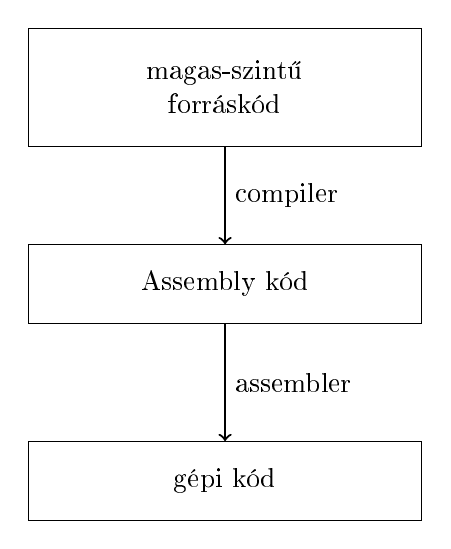
\begin{tikzpicture}
		% High-level source code
		\node[block, minimum width=5cm, minimum height=1.5cm] (highlevel) at (0,0) {};
		\node[align=center] at (highlevel) {magas-szintű\\forráskód};
		
		% Compiler
		\node[block, minimum width=5cm, minimum height=1cm] (compiler) at (0,-2.5) {};
		\node[align=center] at (compiler) {Assembly kód};
		
		% Assembly source code
		\node[block, minimum width=5cm, minimum height=1cm] (assembly) at (0,-5) {};
		\node[align=center] at (assembly) {gépi kód};
		
		% Arrows
		\draw[->, thick] (highlevel.south) -- (compiler.north) node[midway, right] {compiler};
		\draw[->, thick] (compiler.south) -- (assembly.north) node[midway, right] {assembler};
	\end{tikzpicture}
	\caption{A forráskód állapotának szakaszai}
\end{figure}

\section{Fajtái}

A programozási nyelveket háromféle csoportba oszthatjuk attól függően, milyen stratégiát követ az adott nyelv fordítóprogramja.

\subsection{Fordított programozási nyelvek}

Léteznek az ún. \textbf{fordított programozási nyelvek} (\textit{compiled programming languages}, \ref{compiledlang}. ábra), melyeknek fordítóprogramja generál egy, a gépen közvetlenül futtatható állományt. A fordítás folyamata lassabb, azonban a létrejött program végrehajtása gyors. Ha hiba merül fel, két időszakaszban jelentkezhetnek ezek.
\begin{itemize}
	\item \textbf{Fordítási idő}ben történik (\textit{compile time}), ha a compiler veszi észre, jelez róla vissza -- ekkor megszakítja a fordítást. Az ilyen hibát fordítási idejű hibának hívjuk.
	\item \textbf{Futási idő}ben történik (\textit{run time} vagy \textit{runtime}), ha a fordítás sikeres volt, létrejött a futtatható gépi kód, de működés közben elszáll. Ezek a futási idejű hibák.
\end{itemize}

Az ilyen nyelvekben a forráskód alaposabb ellenőrzése erősen javasolt.

További előnye a fordított nyelveknek, hogy a fordító képes a \textbf{tárgykódot optimalizálni}, akár az adott platformra specifikusan. Hátránya sajnos ebben is rejlik, hiszen \textbf{minden platformra külön-külön le kell fordítanunk}.

\begin{figure}[h!]
	\centering
	\begin{tikzpicture}
		\node[block, minimum width=2.5cm, minimum height=1cm] (src) at (-0.5,0) {};
		\node[align=center] at (src) {forráskódok};
		
		\node[block, minimum width=3.5cm, minimum height=1cm] (compiler) at (4,0) {};
		\node[align=center] at (compiler) {\textbf{fordítóprogram}};
		
		\node[block, minimum width=2.5cm, minimum height=2cm] (input) at (10,3) {};
		\node[align=center] at (input) {bemenet, \\ környezet \\ eseményei};
		
		\node[block, minimum width=2.5cm, minimum height=1.5cm] (obj) at (10,0) {};
		\node[align=center] at (obj) {tárgykód \\ (object code)};
		
		\node[block, minimum width=4cm, minimum height=2cm] (output) at (10,-3) {};
		\node[align=center] at (output) {kimenet, \\ program által \\ kiváltott események};
		
		\node[selection, minimum width=4cm, minimum height=3cm] (compiletime) at (4,0) {};
		\node at (4, -1.25) {\textit{fordítási idő}};
		
		\node[selection, minimum width=5cm, minimum height=10cm] (runtime) at (10,0) {};
		\node at (10,-4.75) {\textit{futási idő}};
		
		\draw[->, thick] (src.east)      -- (compiler.west) node[midway, right] {};
		\draw[->, thick] (compiler.east) -- (obj.west)      node[midway, right] {};
		\draw[->, thick] (input.south)   -- (obj.north)     node[midway, right] {};
		\draw[->, thick] (obj.south)     -- (output.north)  node[midway, right] {};
	\end{tikzpicture}
	\caption{Fordítás és végrehajtás}
	\label{compiledlang}
\end{figure}

Tipikusan ilyen nyelvek: C, C++, Haskell, Ada, \dots

\subsection{Értelmezett programozási nyelvek}

A másik nagy csoportot képezik az \textbf{értelmezett} vagy \textbf{interpretált programozási nyelvek} (\ref{interpretedlang}. ábra). Ez némi rugalmasságot enged meg a fordított nyelvekkel szemben. Itt a fordító sorrol sorra hajtja végre az utasításokat és ott áll meg, ahol a hiba jelentkezik -- azaz, \textbf{csak futási idő van}. További következménye, hogy jellemzően \textbf{jelentősen lassabb a végrehajtás}. Cserébe \textbf{minden platformon azonnal futtatható}, ahol az interpreter rendelkezésre áll.

\begin{figure}[h!]
	\centering
	\begin{tikzpicture}
		\node[block, minimum width=2.5cm, minimum height=1cm] (src) at (-0.5,0) {};
		\node[align=center] at (src) {forráskódok};
		
		%\node[block, minimum width=3.5cm, minimum height=1cm] (compiler) at (4,0) {};
		%\node[align=center] at (compiler) {\textbf{fordítóprogram}};
		
		\node[block, minimum width=2.5cm, minimum height=2cm] (input) at (10,3) {};
		\node[align=center] at (input) {bemenet, \\ környezet \\ eseményei};
		
		\node[block, minimum width=2.5cm, minimum height=1.5cm] (obj) at (10,0) {};
		\node[align=center] at (obj) {\textbf{értelmező} \\ (interpreter)};
		
		\node[block, minimum width=4cm, minimum height=2cm] (output) at (10,-3) {};
		\node[align=center] at (output) {kimenet, \\ program által \\ kiváltott események};
		
		%\node[selection, minimum width=4cm, minimum height=3cm] (compiletime) at (4,0) {};
		%\node at (4, -1.25) {\textit{fordítási idő}};
		
		\node[selection, minimum width=5cm, minimum height=10cm] (runtime) at (10,0) {};
		\node at (10,-4.75) {\textit{futási idő}};
		
		\draw[->, thick] (src.east)      -- (obj.west)      node[midway, right] {};
		%\draw[->, thick] (compiler.east) -- (obj.west)      node[midway, right] {};
		\draw[->, thick] (input.south)   -- (obj.north)     node[midway, right] {};
		\draw[->, thick] (obj.south)     -- (output.north)  node[midway, right] {};
	\end{tikzpicture}
	\caption{Értelmezés}
	\label{interpretedlang}
\end{figure}

Tipikusan ilyen nyelvek: Python, Perl, PHP, JavaScript, \dots

\subsection{Fordítás végrehajtás közben}

Létezik a két stratégiának az ötvözete, a \textbf{fordítás végrehajtás közben} (angolul \textit{just-in-time (JIT) compilation}).

Hasonlóan a fordított programozási nyelvekhez, a fordítási és futási idő elkülönül. A fordítóprogram gépi kód helyett \textbf{bájtkód}ra (\textit{bytecode}) fordítja le a forráskódot. Ezután a \textbf{virtuális gép} (\textit{virtual machine}) végrehajtja a bájtkód utasításait. Azonban felmerülnek bizonyos problémák.
\begin{enumerate}
	\item Ha a virtuális gép \textit{futási időben értelmezi} a bájtkódot, az ugyanolyan lassan történne, mint egy hagyományos értelmezett nyelv esetében.
	\item Ha \textit{végrehajtás előtt fordítjuk le} teljesen a bájtkódot gépi kódra, az túl nagy kezdeti lassulást eredményezne.
\end{enumerate}

Éppen ezért a következő stratégiát követi a virtuális gép.
\begin{enumerate}
	\item Kezdetben értelmezi, interpretálja a bájtkódot.
	\item Futási időben statisztikákat gyűjt a leggyakrabban lefutó kódrészletekről. Ezeket ``\textit{hot spot}''-oknak nevezzük.
	\item Ezeket lefordítja gépi kódra.
	\item Így a következő alkalommal a lefordított kódrészlet fut az értelmezés helyett.
\end{enumerate}

További előnye, hogy a JIT fordító futási időben gyűjtött információkat is figyelembe vehet a kódoptimalizálásnál. Ilyenekhez a klasszikus fordítóprogram nem fér hozzá!

Ugyanakkor, a bájtkódok végrehajtása jellemzően még így is lassabb a gépi kódhoz képest, de ez sepciális alkalmazási
területeket leszámítva nem baj.

Tipikusan ilyen nyelvek: C\#, Java.

\begin{figure}[h!]
	\centering
	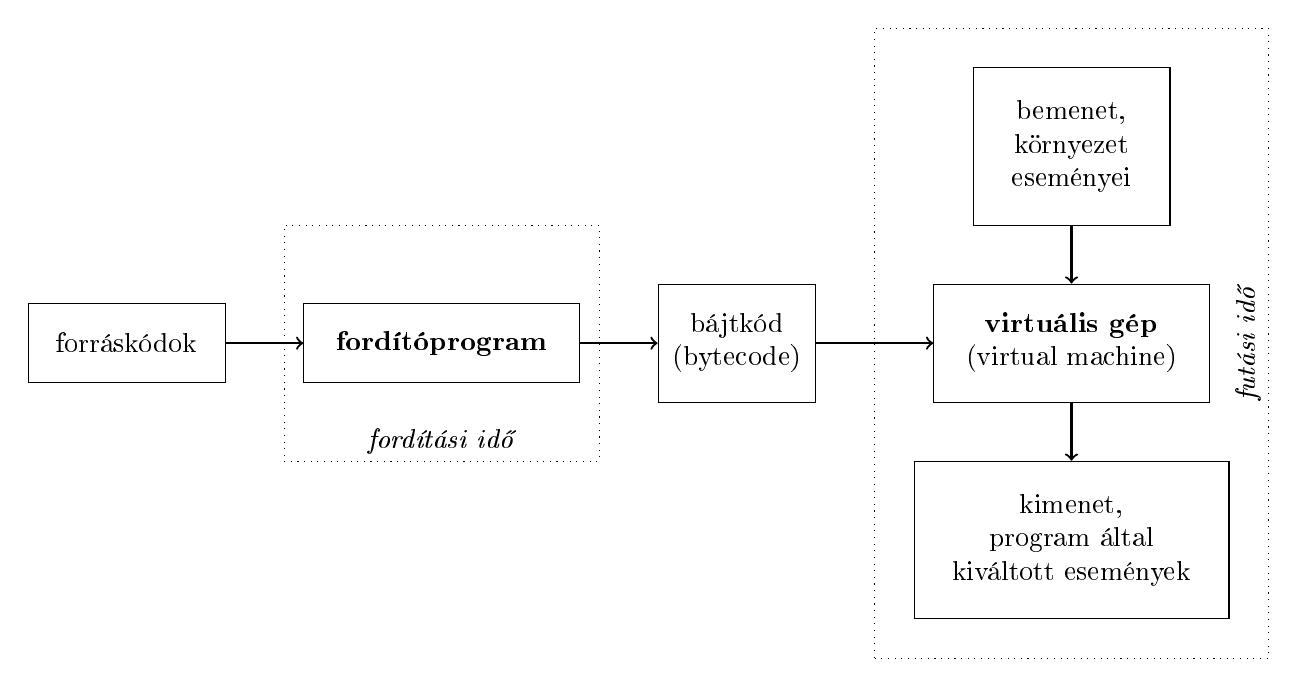
\begin{tikzpicture}
		\node[block, minimum width=2.5cm, minimum height=1cm] (src) at (-2,0) {};
		\node[align=center] at (src) {forráskódok};
		
		\node[block, minimum width=3.5cm, minimum height=1cm] (compiler) at (2,0) {};
		\node[align=center] at (compiler) {\textbf{fordítóprogram}};
		
		\node[block, minimum width=2cm, minimum height=1.5cm] (bytecode) at (5.75,0) {};
		\node[align=center] at (bytecode) {bájtkód \\ (bytecode)};
		
		\node[block, minimum width=2.5cm, minimum height=2cm] (input) at (10,2.5) {};
		\node[align=center] at (input) {bemenet, \\ környezet \\ eseményei};
		
		\node[block, minimum width=3.5cm, minimum height=1.5cm] (obj) at (10,0) {};
		\node[align=center] at (obj) {\textbf{virtuális gép} \\ (virtual machine)};
		
		\node[block, minimum width=4cm, minimum height=2cm] (output) at (10,-2.5) {};
		\node[align=center] at (output) {kimenet, \\ program által \\ kiváltott események};
		
		\node[selection, minimum width=4cm, minimum height=3cm] (compiletime) at (2,0) {};
		\node at (2, -1.25) {\textit{fordítási idő}};
		
		\node[selection, minimum width=5cm, minimum height=8cm] (runtime) at (10,0) {};
		\node[rotate=90] at (12.25,0) {\textit{futási idő}};
		
		\draw[->, thick] (src.east)      -- (compiler.west) node[midway, right] {};
		\draw[->, thick] (compiler.east) -- (bytecode.west) node[midway, right] {};
		\draw[->, thick] (bytecode.east) -- (obj.west)      node[midway, right] {};
		\draw[->, thick] (input.south)   -- (obj.north)     node[midway, right] {};
		\draw[->, thick] (obj.south)     -- (output.north)  node[midway, right] {};
	\end{tikzpicture}
	\caption{JIT-fordítás}
\end{figure}

\begin{center}
	\begin{tabular}{c|cc}
		%\hline
		\textbf{Nyelv} & \textbf{Bájtkód} & \textbf{Virtuális gép} \\
		\hline
		C\# & Common Intermediate Language (CLI) & Common Language Runtime (CLR) \\
		%\hline
		Java & Java bytecode & Java Virtual Machine (JVM) \\
		%\hline
	\end{tabular}
\end{center}

\section{Fejlődése}

%1957-ben jelent meg a legelső compiler, ami a Fortran nyelvhez készült, 18 emberévnyi munka után.

\begin{itemize}
	\item 1957: Első \textbf{Fortran compiler} -- 18 emberévnyi munka
	\item Azóta fejlődött a \textbf{formális nyelvek és automaták elmélete}.
	\item Ma: A fordítóprogramok létrehozásának egy része \textbf{automatizálható} elemzőgenerátorokkal.
	\begin{itemize}
		\item A programszöveg elemi egységekre (tokenekre) bontása
		\item A programszöveg formai helyességének vizsgálata
	\end{itemize}
	\item A további ellenőrzések és a kódgenerálás nem automatizálható, de az implemetációt \textbf{keretrendszerek} segíthetik.
	\item A \textbf{kódoptimalizálás} (és a hozzá szükséges elemzések) komoly kihívás.
\end{itemize}

\section{Logikai felépítése}

Két fázisból áll a fordítás: az \textbf{analízis}ből és \textbf{szintézis}ből. Az egyes részeket és alrészeket önálló fejezetek is részletezik, itt csak egy rövid áttekintést nyújtunk.

A vizuális összefoglaló a \ref{compilation}. ábrán található.

\subsection{Analízis}

Az analízis \textit{előfeldolgozás}t hajt végre a bemeneti forráskódon. Ellenőrzi, hogy lexikálisan, szintaktikusan, illetve szemantikusan helyes-e a kódunk. Ha ez nincs így, a megfelelő helyen hibát dob.

\subsubsection{Lexikális elemzés}

\begin{itemize}
	\item \textit{Feladat}: A forrásszöveg elemi egységekre, ún. \textbf{token}ekre bontása. Idegen szóval ez a \textbf{tokenizáció}.
	\item \textit{Bemenet}: karaktersorozat
	\item \textit{Kimenet}: tokenek sorozata + lexikális hibák
	\item \textit{Eszközök}: reguláris kifejezések, véges determinisztikus automaták
\end{itemize}

\begin{figure}[h!]
	\centering
	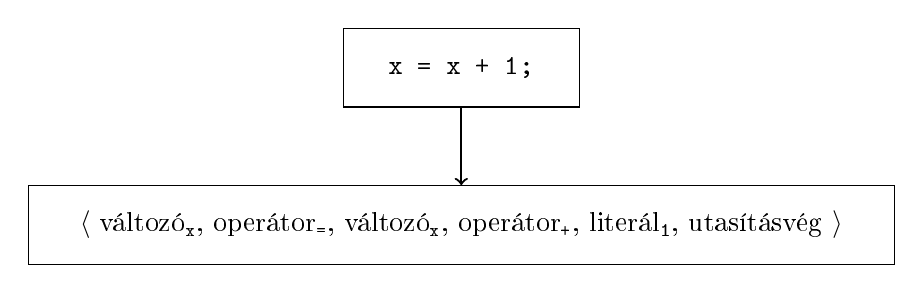
\begin{tikzpicture}
		\node[block, minimum width=3cm, minimum height=1cm] (input) at (0,0) {};
		\node at (input) {\texttt{x = x + 1;}};
		
		\node[block, minimum width=11cm, minimum height=1cm] (output) at (0, -2) {};
		\node at (output) {
			$\langle$
			változó\textsubscript{\texttt{x}}, 
			operátor\textsubscript{\texttt{=}}, 
			változó\textsubscript{\texttt{x}}, 
			operátor\textsubscript{\texttt{+}}, 
			literál\textsubscript{\texttt{1}}, 
			utasításvég
			$\rangle$
		};
	
	\draw[->, thick] (input.south) -- (output.north);
	\end{tikzpicture}
	\caption{Helyes lexikális elemzés eredménye}
\end{figure}


\subsubsection{Szintaktikus elemzés}

\begin{itemize}
	\item \textit{Feladat}: A forrásszöveg szerkezetének felderítése, formai ellenőrzése.
	\item \textit{Bemenet}: tokenek sorozata
	\item \textit{Kimenet}: szintaxisfa + szintaktikus hibák
	\item \textit{Eszközök}: környezetfüggetlen nyelvtanok, veremautomaták
\end{itemize}

\begin{figure}[h!]
	\centering
	\begin{tikzpicture}
		\node[block, minimum width=11cm, minimum height=1cm] (input) at (0, 0) {};
		\node[align=center] at (input) {
			$\langle$
			változó\textsubscript{\texttt{x}}, 
			operátor\textsubscript{\texttt{=}}, 
			változó\textsubscript{\texttt{x}}, 
			operátor\textsubscript{\texttt{+}}, 
			literál\textsubscript{\texttt{1}}, 
			utasításvég
			$\rangle$
		};
	
		\node[block, minimum width=14cm, minimum height=6cm] (output) at (0,-4) {};
		\node at (output) {
			\begin{tikzpicture}[sibling distance=1em]
				\Tree
				[.{Utasítás}
					[.{Kifejezés}
						[.{Kifejezés}
							{változó\textsubscript{\texttt{x}}}
						]
						{operátor\textsubscript{\texttt{=}}}
						[.{Kifejezés}
							[.{Kifejezés}
								{változó\textsubscript{\texttt{x}}}
							]
							{operátor\textsubscript{\texttt{+}}}
							[.{Kifejezés}
								{literál\textsubscript{\texttt{1}}}
							]
						]
					]
					{utasításvég}
				]
			\end{tikzpicture}
		};
		
		\draw[->, thick] (input.south) -- (output.north);
	\end{tikzpicture}
	\caption{Helyes szintaktikus elemzés eredménye}
\end{figure}

Az alábbi környezetfüggetlen nyelv határozza meg a szintaxist. Ezen nyelvnek a terminális szimbólumai a tokenek (lexikális elemek).
\begin{flalign*}
	\text{<Utasítás>} &::= \text{<Kifejezés> utasításvég}
	\\
	\text{<Kifejezés>} &::= \text{változó | literál | <Kifejezés> operátor <Kifejezés>}
\end{flalign*}

\subsubsection{Szemantikus elemzés}

\begin{itemize}
	\item \textit{Feladat}: A statikus szemantika (pl. változók deklaráltsága, típushelyesség stb.) ellenőrzése
	\item \textit{Bemenet}: szintaxisfa
	\item \textit{Kimenet}: \textbf{szintaxisfa attribútumokkal}, \textbf{szimbólumtábla} + szemantikus hibák
	\item \textit{Eszközök}: \textbf{attribútumnyelvtanok}
\end{itemize}

\begin{figure}[h!]
	\centering
	\begin{tabular}{|l|l|}
		\hline
		Név ~~~~~ & Típus ~~~~~ \\
		\hline
		\texttt{x} & \texttt{int} \\
		\hline
	\end{tabular}
	\caption{Szimbólumtáblázat. Általában több információt is tartalmaz.}
\end{figure}

\begin{figure}[h!]
	\centering
	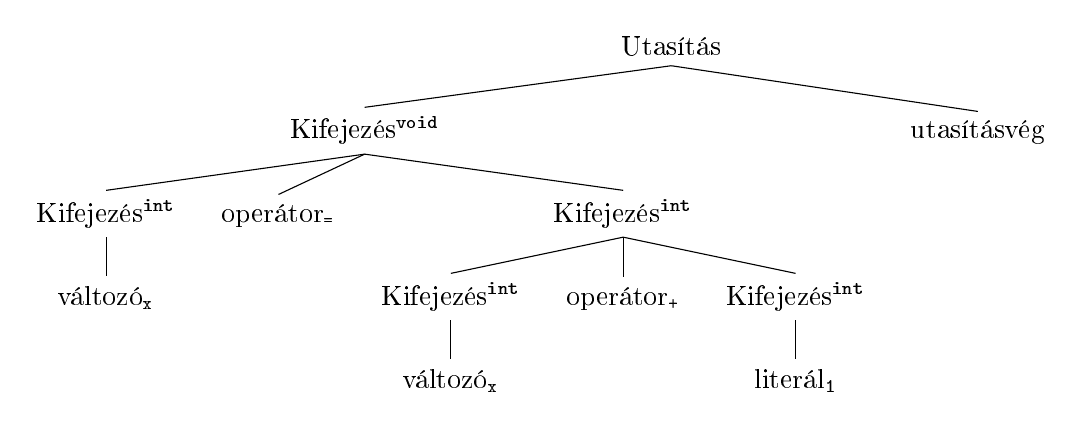
\begin{tikzpicture}[sibling distance=1em]
		\Tree
		[.{Utasítás}
		[.{Kifejezés\textsuperscript{\texttt{void}}}
		[.{Kifejezés\textsuperscript{\texttt{int}}}
		{változó\textsubscript{\texttt{x}}}
		]
		{operátor\textsubscript{\texttt{=}}}
		[.{Kifejezés\textsuperscript{\texttt{int}}}
		[.{Kifejezés\textsuperscript{\texttt{int}}}
		{változó\textsubscript{\texttt{x}}}
		]
		{operátor\textsubscript{\texttt{+}}}
		[.{Kifejezés\textsuperscript{\texttt{int}}}
		{literál\textsubscript{\texttt{1}}}
		]
		]
		]
		{utasításvég}
		]
	\end{tikzpicture}
	\caption{Szintaxisfa attribútumokkal}
\end{figure}

\newpage

\subsection{Szintézis}

\subsubsection{Kódgenerálás}

\begin{itemize}
	\item \textit{Feladat}: Alacsonyabb szintű belső reprezentációkra, végül \textbf{tárgykód}dá alakítja a programot
	\item \textit{Bemenet}: szintaxisfa attribútumokkal, szimbólumtábla
	\item \textit{Kimenet (az utolsó menetben)}: \textbf{tárgykód}
	\item \textit{Eszközök}: \textbf{kódgenerálási sémák}
\end{itemize}

Közvetlenül gépi kódot csak nagyon indokolt esetben érdemes generálni. Helyette Assembly kód (pl. valamely platform Assembly nyelve vagy LLVM) generálható, amit assemblerekkel fordítunk tovább.

Megemlíthetjük az ún. \textbf{transzláció}t is. Ez magas szintű nyelvek közti fordítást jelent. Ez lehet végcél (pl. projektek portolása esetén egyik nyelvről a másikra), ugyanakkor elterjedt nyelvekre való fordítás esetén használhatjuk azok fordítóit a gépi kód / bájtkód előállításához.

\subsubsection{Optimalizáció}

\begin{itemize}
	\item \textit{Feladat}: Kód átalakítása hatékonyságnövelés céljából (pl. sebességnövelés, memóriaigény csökkentés)
	\item \textit{Bemenet}: belső reprezentáció / tárgykód
	\item \textit{Kimenet (az utolsó menetben)}: belső reprezentáció / tárgykód
	\item \textit{Eszközök}: \textbf{Statikus elemzés}, \textbf{transzformációs keretrendszerek}
\end{itemize}

Egyes compilerek több lépésben is optimalizálhatják a kódot. 

Ahogy megtárgyaltuk, a szintézis fázisa úgy kezdődik, hogy rendelkezésünkre áll a szintaxisfa. Ezen ún. \textbf{magas szintű optimalizáció}t hajtanak végre, így kapunk egy optimalizált szintaxisfát\footnote{El tudjuk képzelni, hogy milyen matematikai vonatkozásai lehetnek ennek: egy fagráfot kevesebb úttal vagy csúccsal ``írjunk fel'' úgy, hogy az ezen gráf által felírt ``program'' ekvivalens maradjon az eredetivel. (A megfogalmazás természetesen matematikailag pontatlan, csupán a szemléltetés céljából raktam ide.)}. Ez alapján megtörténik a kódgenerálás, létrejön az Assembly kód. Végül ezt az Assembly kódot optimalizáljuk (\textbf{alacsony szintű optimalizálás}).

\begin{figure}
	\centering
	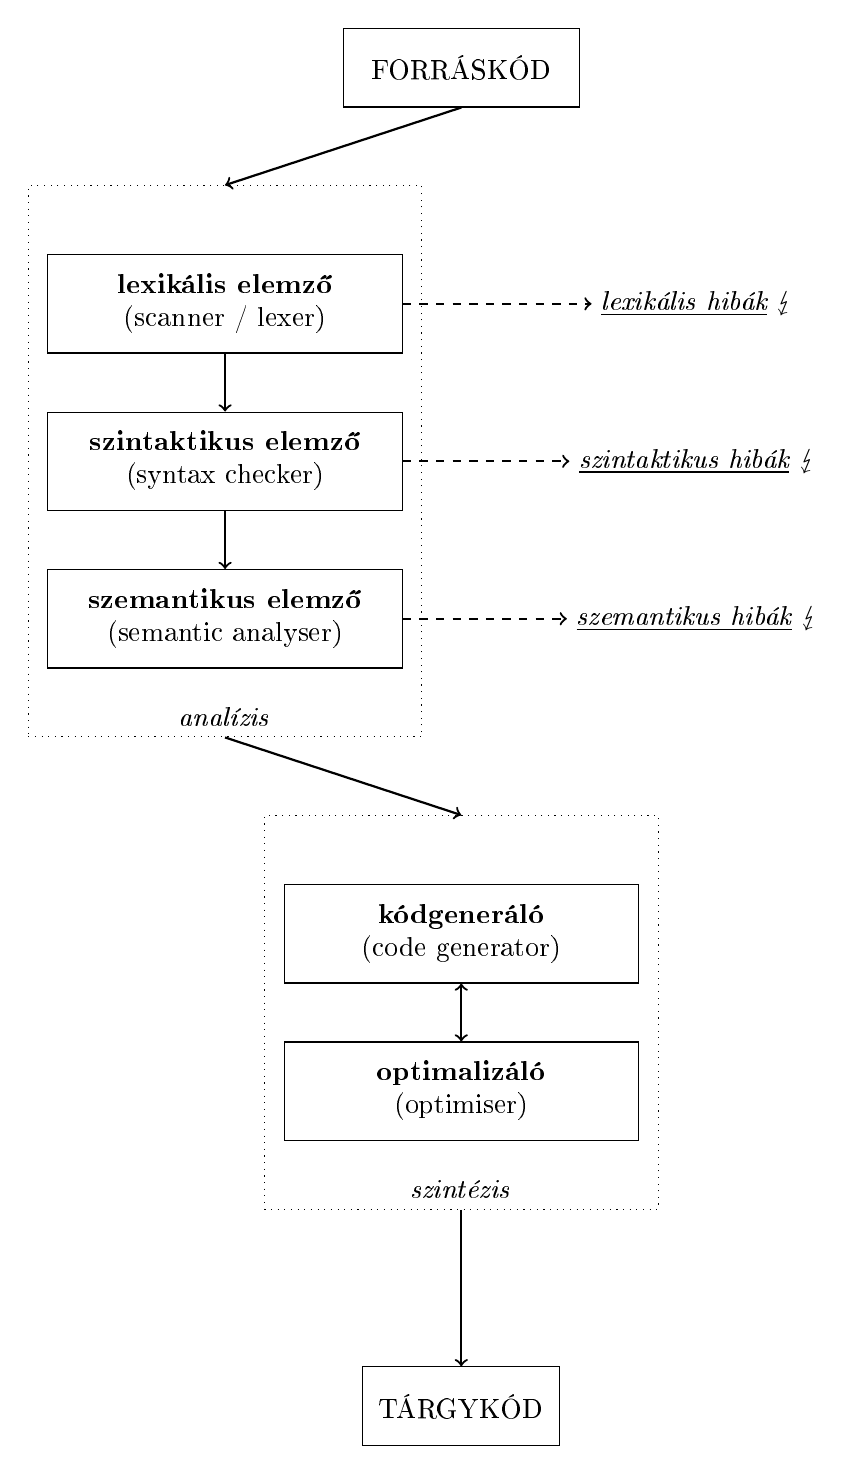
\begin{tikzpicture}
		\node[block, minimum width=3cm, minimum height=1cm] (src) at (0,1) {};
		\node[align=center] at (src) {FORRÁSKÓD};
		
		\node[selection, minimum width=5cm, minimum height=7cm] (analysis) at (-3, -4) {};
		
		\node[block, minimum width=4.5cm, minimum height=1.25cm] (lexer) at (-3,-2) {};
		\node[align=center] at (lexer) {\textbf{lexikális elemző} \\ (scanner / lexer)};
		
		\node[align=center] (lexererror) at (3, -2) {\textit{\underline{lexikális hibák} $\lightning$}};
		
		\node[block, minimum width=4.5cm, minimum height=1.25cm] (syntax) at (-3,-4) {};
		\node[align=center] at (syntax) {\textbf{szintaktikus elemző} \\ (syntax checker)};
		
		\node[align=center] (syntaxerror) at (3, -4) {\textit{\underline{szintaktikus hibák} $\lightning$}};
		
		\node[block, minimum width=4.5cm, minimum height=1.25cm] (semantics) at (-3,-6) {};
		\node[align=center] at (semantics) {\textbf{szemantikus elemző} \\ (semantic analyser)};
		
		\node[align=center] (semanticerror) at (3, -6) {\textit{\underline{szemantikus hibák} $\lightning$}};
		
		\node[block, minimum width=4.5cm, minimum height=1.25cm] (codegen) at (0,-10) {};
		\node[align=center] at (codegen) {\textbf{kódgeneráló} \\ (code generator)};
		
		\node[block, minimum width=4.5cm, minimum height=1.25cm] (optimiser) at (0,-12) {};
		\node[align=center] at (optimiser) {\textbf{optimalizáló} \\ (optimiser)};
		
		\node[selection, minimum width=5cm, minimum height=5cm] (synthesis) at (0, -11) {};
		
		\node[align=center] at (-3,-7.25) {\textit{analízis}};
		\node[align=center] at (0, -13.25) {\textit{szintézis}};
		
		\node[block, minimum width=2.5cm, minimum height=1cm] (obj) at (0,-16) {};
		\node[align=center] at (obj) {TÁRGYKÓD};
		
		\draw[->, thick] (src.south)      -- (analysis.north) node[midway, right] {};
		
		\draw[->, thick] (lexer.south)    -- (syntax.north)    node[midway, right] {};
		\draw[->, thick] (syntax.south)   -- (semantics.north) node[midway, right] {};
		
		\draw[->, thick, dashed] (lexer.east)  -- (lexererror.west) node[midway, right] {};
		\draw[->, thick, dashed] (syntax.east)  -- (syntaxerror.west) node[midway, right] {};
		\draw[->, thick, dashed] (semantics.east)  -- (semanticerror.west) node[midway, right] {};
		
		\draw[<->, thick] (codegen) -- (optimiser);
		
		\draw[->, thick] (analysis.south) -- (synthesis.north) {};
		
		\draw[->, thick] (synthesis.south) -- (obj.north) {};
	\end{tikzpicture}
	\caption{A fordítóprogramok logikai felépítése}
	\label{compilation}
\end{figure}

\newpage

\section{Szerkesztés és végrehajtás}

Általában amikor programot írunk, modularizálva írjuk meg azt, azaz több, kisebb részekre bontjuk fel -- legtöbbször \textbf{könyvtárak}, \textbf{csomagok} formájában. Ezen összetevők gyakran hivatkoznak egymásra, emiatt elengedhetetlen, hogy el is érjék egymást. Ezt oldja meg a(z) \textbf{(össze)szerkesztés} vagy \textbf{linkelés}.

A mai rendszereken kétféle stratégia létezik a könyvtárak összeszerkesztéséhez.

\begin{enumerate}
	\item \underline{Statikus szerkesztés}
	
	Nagy vonalakban azt jelenti, hogy mindazon \textbf{könyvtárakat, csomagokat}, melyeket felhasználunk a programunkban, \textbf{``beleégetjük'' a gépi kódba}. Tipikusan ez történik, amikor C-ben include-oljuk az \texttt{stdio.h} könyvtárat. Hiába csak a \texttt{printf} függvényt használjuk fel, minden más is bekerül a binárisba.
	
	Ez előnyös lehet, mivel csökkenti a külső függőségeket (akár használhatjuk a programunkat olyan rendszeren, amin nincs telepítve a \texttt{glibc}). Hátránya, hogy jelentősen megnövelheti a futtatható fájl méretét.
	
	A statikus könyvtárak tipikus kiterjesztései: \texttt{.a}, \texttt{.lib}.
	
	\item \underline{Dinamikus szerkesztés}
	
	Futási időben éri el a hivatkozott függvényeket, osztályokat, stb. Előnye, hogy kisebb lesz a futtatandó fájl mérete. Hátránya pedig, hogy meg kell győződnünk futtatás előtt, hogy telepítve vannak-e a szükséges \textbf{függőségek}.
	
	A dinamikus könyvtárak tipikus kiterjesztései: \texttt{.so} (\textit{shared object}), \texttt{.dll} (\textit{dynamically linked library}).
	
	Ha visszaemlékszünk az \textit{Objektumelvű programozás} c. tárgyból tanultakra, a gyakorlatokon használtuk a \texttt{TextFileReader.dll} könyvtárat, ami (a mostani tudásunkkal összevetve) egy dinamikusan linkelt könyvtár.
\end{enumerate}

A programunk futtatása, végrehajtása esetén a \textbf{teljes futtatható állományt betöltjük a fájlrendszerből}. Ha dinamikus könyvtárakat is használunk, ezek is betöltésre kerülnek.
\chapter{Lexikális elemzés}

\section{A tokenizáció}

Adott az alábbi karakterlánc:
\begin{center}
	\texttt{x = (x + 2) * 3;}
\end{center}
A feladat, hogy hogyan állapíthatjuk meg a benne lévő tokeneket?

Számunkra ránézésre nyilvánvaló, hogy a helyes tokenizáció a következő:
\begin{center}
	$\langle$ \texttt{x}, \texttt{=}, \texttt{(}, \texttt{x}, \texttt{+}, \texttt{2}, \texttt{)}, \texttt{*}, \texttt{3}, \texttt{;} $\rangle$.
\end{center}

Ezt kell valahogy a ``számítógép nyelvén'' kifejeznünk. Megállapítunk bizonyos tulajdonságokat, melyekkel kizárásos alapon kiválaszthatjuk a tokeneket.
\begin{itemize}
	\item \textbf{Aminek a belső szerkezete fontos, nem lehet token!} \\
	Például az értékadásnak van bal és jobb oldala, mindkettőnek megvannak a rá vonatkozó szabályai. 
	\begin{center}
		$\langle$ \texttt{x}, \texttt{=}, \texttt{(x + 2) * 3}, \texttt{;} $\rangle$ $\lightning$
	\end{center}
	
	Mivel az értékadás önmaga is egy utasítás, amire szintén vonatkoznak szabályok, emiatt az alábbi tokenizáció sem helyes.
	\begin{center}
		$\langle$ \texttt{x = (x + 2) * 3}, \texttt{;} $\rangle$ $\lightning$
	\end{center}
	
	\item \textbf{Aminek a formája nem írható le reguláris kifejezéssel, nem lehet token!} \\
	Tipikus példája ennek a helyes zárójelezések nyelve, ami környezetfüggetlen grammatikával írható le.
	\begin{center}
		$\langle$ \texttt{x}, \texttt{=}, \texttt{(x + 2)}, \texttt{*}, \texttt{3}, \texttt{;} $\rangle$ $\lightning$
	\end{center}
\end{itemize}

Következő probléma: a \textbf{fehérelválasztók} (\textit{whitespaces}). A legtöbb programozási nyelvnél a szóközök, tabulátorok és újsorok \textbf{nem alkotnak tokeneket}, csak más tokenek elválasztására valók. A lexikális elemzőnek fel kell ismernie ezeket, de nem kell továbbítania a szintaktikus elemző felé.

Ezalól kivételt képeznek a \textbf{behúzásra} (vagy indentációra) \textbf{érzékeny nyelvek}, mint a Python vagy a Haskell. Az elemzőnek a \textbf{sorok behúzását számon kell tartania}. Növekvő behúzás jelenti a blokknyitó tokent (C-ben \texttt{\{}), a csökkenő behúzás meg a blokkzáró tokent (C-ben \texttt{\}}).

Érdekességként megemlítjük a \href{https://www.wikiwand.com/en/Whitespace\_(programming\_language)}{\textit{Whitespace}} nyelvet, amiben kizárólag a fehérelválasztóknak van jelentése.

Ahogy korábban megállapítottuk, token csak az lehet, amit leírhatunk reguláris kifejezéssel. Bizonyos reguláris kifejezések elsőbbséget élveznek a többivel szemben -- nevezetesen azok, melyekkel kulcsszavakat írunk le. Tehát a konkrétabbak előrébb, az általánosabbak hátrébb kerülnek a felsorolásban.

\begin{figure}[h!]
	\centering
	\begin{tabular}{l|ll}
		%\hline
		\textbf{Reguláris kifejezés} & \textbf{Példák} & \textbf{Token típus} \\
		\hline
		\texttt{while} & \textit{while} & kulcsszó a While nyelvben \\
		%\hline
		\texttt{[a-zA-Z][a-zA-Z0-9\_]*} & \textit{x}, \textit{apple123}, \textit{list\_length} & azonosító \\
		%\hline
		\texttt{[+-]?[0-9]+} & \textit{0}, \textit{123}, \textit{-2}, \textit{+100} & egész számliterál \\
		%\hline
		\texttt{[ \textbackslash t\textbackslash n]+} & (fehérelválasztók nemüres sorozata) & -- \\
		%\hline
		\texttt{"//".*} & \textit{// Ez egy megjegyzés} & -- \\
		%\hline
	\end{tabular}
	\caption{Definíció reguláris kifejezéssekkel}
\end{figure}

\section{A lexikális elemzés elvei}

\begin{itemize}
	\item \textbf{Leghosszabb illeszkedés elve}\\
	A leghosszabban illeszkedő karaktersorozatból képzünk tokent.
	
	Pl. \texttt{w|hile}, \texttt{wh|ile}, \dots, \texttt{whil|e}$\to$ Hiába helyes azonosító szimbólum a \texttt{w}, \texttt{wh}, \dots, \texttt{whil}, mégis folytatni kell a keresést.
	
	\item \textbf{Prioritás elve} \\
	Ha a leghosszabban illeszkedő karaktersorozat több reguláris kifejezésre is illeszkedhet, a sorrendben korábban álló ``nyer''.
	
	Pl. \texttt{while|} $\to$ Lehet kulcsszó is, lehet azonosító is. Mivel kulcsszóként korábban definiáltuk, így ez élvez elsőbbséget.
\end{itemize}

\section{Implementációja}

A reguláris kifejezések átalakíthatók \textbf{véges determinisztikus automatá}vá.

\tikzset{
	->, % makes the edges directed
	%>=stealth’, % makes the arrow heads bold
	node distance=3cm, % specifies the minimum distance between two nodes. Change if necessary.
	%every state/.style={thick}, % sets the properties for each ’state’ node
	initial text=$ $ % sets the text that appears on the start arrow
}

\begin{minipage}{0.33\linewidth}
	\begin{center}
		\texttt{[a-z][a-z0-9]*}
	\end{center}
\end{minipage}
\begin{minipage}{0.66\linewidth}
	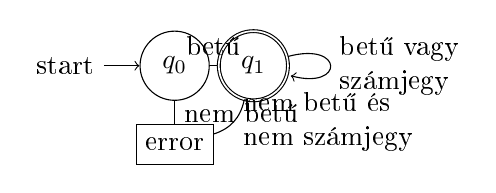
\begin{tikzpicture}
		%\node[state] (q1) {normal};
		%\node[state, initial, right of=q1] (q2) {start};
		%\node[state, accepting] at (1.5, 2) (q3) {accept};
		
		\node[state, initial] (q0) {$q_0$};
		\node[state, accepting, right of=q0] (q1) {$q_1$};
		\node[block, below of=q0, minimum width=0.7cm, minimum height=0.5cm] (error) {error};
		
		\draw (q0) edge[above] node{betű} (q1);
		\draw (q1) edge[loop right] node[align = left]{betű vagy \\ számjegy} (q1);
		\draw (q0) edge[right] node{nem betű} (error);
		\draw (q1) edge[right, bend left] node[align = left] {nem betű és \\ nem számjegy} (error);
	\end{tikzpicture}
\end{minipage}

A VDA implementációja történhet \textbf{elágazásokkal}, amelynek a struktogramja itt látható (a $\mathbb{K}$ jelöli a \texttt{char} adattípust).

\begin{stuki*}[14cm]{vda::process(next : $\mathbb{K})$}
	\begin{CASE}{2}{2}
		\WHEN{\stm{state = q_0}}
		\begin{IF}{1}{\stm{next = \texttt{'a'} \lor \dots}}
			\stm{state := q_1}
			\ELSE
			\stm{state := error}
		\end{IF}
		\WHEN{\stm{state = q_1}}
		\begin{IF}{1}{\stm{next = \texttt{'a'} \lor \dots \lor next = \texttt{'0'} \lor \dots}}
			\stm{state := q_1}
			\ELSE
			\stm{state := error}
		\end{IF}
	\end{CASE}
\end{stuki*}

\begin{lstlisting}[style=cppstyle, caption={VDA implementációja elágazásokkal}]
void vda::process(char next) 
{
	if (state == q0) {
		if (next == 'a' || ...) {
		    state = q1;
		} else {
		    state = error;
		}
	} else if (state == q1) {
		if (next == 'a' || ... || next == '0' || ...) {
		    state = q1;
		} else {
		    state = error;
		}
	}
}
\end{lstlisting}

Megoldható ugyanakkor \textbf{táblázattal} is.

\begin{figure}[h!]
	\centering
	\begin{tabular}{c||cc}
		%\hline
		& $q_0$ & $q_1$ \\
		\hline\hline
		\texttt{a} & $q_1$ & $q_1$ \\
		\hline
		\vdots & \multicolumn{2}{c}{\vdots} \\
		\hline
		\texttt{0} & error & $q_1$ \\
		\hline
		\vdots & \multicolumn{2}{c}{\vdots} \\
		\hline
		other & error & error \\
		%\hline
	\end{tabular}
	\caption{A VDA táblázata}
\end{figure}

\begin{stuki*}{vda::process$(next : \mathbb{K})$}
	\begin{IF}[80]{1}{\stm{state \neq error}}
		\stm{state := translations[state][next]}
		\ELSE
		\stm*{SKIP}
	\end{IF}
\end{stuki*}

\begin{lstlisting}[style=cppstyle, caption={VDA implementációja táblázattal}]
void vda::process(char next) 
{
	if (state != error) {
		state = transitions[state][next];
	}
}
\end{lstlisting}

%\textbf{\textit{Megjegyzés}}. A \texttt{vda::process} függvényben 

\newpage
\section{Tokenhez csatolt információk}

A felismert tokenekhez a lexikális elemző kiegészítő információkat csatol. Ezeket nevezzük \textbf{kitüntetett szintetizált attribútumok}nak. A jelentősségük a szemantikus elemzésnél fog megjelenni.

\begin{itemize}
	\item \textbf{Minden tokenhez}: a token pozícióját (első karakter sor- és oszlop-, utolsó karakter sor- és oszlopszáma)
	\item \textbf{Azonosítókhoz}: az azonosító szövegét (ez szükséges a szemantikus elemzéshez)
	\item \textbf{Literálokhoz}: a literál értékét (kódgeneráláshoz, kódoptimalizációhoz szükséges)
\end{itemize}

\section{Lexikális hibák}

Lexikális hiba esetén hibajelzést ad a fordító, és \textit{folytatja az elemzést}. A leggyakrabban előforduló hibák:
\begin{itemize}
	\item \underline{Illegális karakter}: A nyelv ábécéjébe nem tartozó karakter az inputszövegben. \\
	Az addig felépített token kiadja, ha volt illeszkedés. 
	Az illegális karaktert követő karakterrel folytatódik az elemzés.
	
	\item \underline{Lezáratlan sztring} \\
	A sor végén derül ki; az őt követő sorban folytatódik az elemzés.
	
	\item \underline{Lezáratlan többsoros megjegyzés} \\
	A fájl végén derül ki; nincs további elemzés.
\end{itemize}

%\section{Szemléltetés}


\chapter{Szintaktikus elemzés}

\section{Grammatikai előfeltételek}

A lexikális elemzés kinyerte a tokenek sorozatát a forrásfájlból. Ebben a lépésben az a feladatunk, hogy ezen tokenekből a ``nyelvtani hierarchiát'', a \textbf{szintaxisfát} állítsuk fel. Ehhez szükségünk vannak a \textbf{környezetfüggetlen nyelvtanok}ra, valamint az ezek elfogadására szolgáló \textbf{veremautomaták}ra.

Szintkaktikus elemzőt manapság nagyon egyszerűen hozhatunk létre különböző generátorok segítségével. Ilyen például a \href{https://www.gnu.org/software/bison/}{Bison}, amit a gyakorlaton is használunk. Ennek a forrásfájljában (pl. \texttt{while.y}) megadjuk a lehetséges tokeneket és definiáljuk a szabályainkat.

Ahhoz, hogy elemezhető nyelvet tudjunk készíteni, a nyelvtanunknak szüksége van arra, hogy bizonyos előfeltételeket teljesítsen.

\begin{enumerate}
	\item \underline{Redukáltság}: Nincsenek ``felesleges'' nemterminálisok. \\
	Mindegyik nemterminálishoz adható olyan levezetés, amiben szerepel, és nem üres terminális sorozatot vezetünk le belőle.
	
	\item \underline{Ciklusmentesség}: Nincs $\prodrule{A}{\text{\textsuperscript{+}\textit{A}}}$ levezetés. \\
	Ciklusos nyelvtan olyan, aminek az egyik bal oldalának levezetéséből visszajuthatunk önmagába. Példa ciklusos (tehát nem jó) nyelvtanra:
	\begin{flalign*}
		& \prodrule{S}{A} \\
		& \prodrule{A}{a \mid B} \\
		& \prodrule{B}{A}.
	\end{flalign*}
	
	\item \underline{Egyértelműség}: Minden szóhoz \textbf{pontosan egy szintaxisfa} tartozik.
	\begin{itemize}
		\item Több levezetés tartozhat egy szóhoz, de a szintaxisfáik legyenek identikusak!
		
		\begin{minipage}{0.5\linewidth}
			\begin{flalign*}
				S \Longrightarrow AB &\Longrightarrow  aB \Longrightarrow ab \\
				S \Longrightarrow AB &\Longrightarrow  Ab \Longrightarrow ab \\
			\end{flalign*}
		\end{minipage}
		\begin{minipage}{0.5\linewidth}
			\begin{forest}
				for tree={parent anchor=south, child anchor=north, l=1em, l sep=1em, s sep=1em, edge={-}}
				[$S$
					[$A$
						[$a$]
					]
					[$B$
						[$b$]
					]
				]
			\end{forest}
		\end{minipage}
		
		\pagebreak
		
		\item Példa nem egyértelmű nyelvtanra: $\prodrule{S}{\texttt{utasítás} \mid SS}$.
		
		\begin{minipage}{0.5\linewidth}
			\begin{forest}
				for tree={ edge={-}}
				[$S$
					[$S$
						[\texttt{utasítás}, tier=terminal]
					]
					[$S$
						[$S$
							[\texttt{utasítás}, tier=terminal]
						]
						[$S$
							[\texttt{utasítás}, tier=terminal]
						]
					]
				]
			\end{forest}
		\end{minipage}
		\begin{minipage}{0.5\linewidth}
			\begin{forest}
				for tree={ edge={-}}
				[$S$
					[$S$
					[$S$
					[\texttt{utasítás}, tier=terminal]
					]
					[$S$
					[\texttt{utasítás}, tier=terminal]
					]
					]
					[$S$
						[\texttt{utasítás}, tier=terminal]
					]
				]
			\end{forest}
		\end{minipage}
		
		Ez a nemegyértelműség feloldható a nyelvtan átalakításával:
		\[ \prodrule{S}{\texttt{utasítás} ~ S \mid \texttt{utasítás}} ~~~ \text{ vagy } ~~~ \prodrule{S}{S ~ \texttt{utasítás} \mid \texttt{utasítás}}. \]
	
		\begin{minipage}{0.5\linewidth}
			\begin{forest}
				for tree={ edge={-}}
				[$S$
				[\texttt{utasítás}, tier=terminal]
				[$S$
				[\texttt{utasítás}, tier=terminal]
				[$S$
				[\texttt{utasítás}, tier=terminal]
				]
				]
				]
			\end{forest}
		\end{minipage}
		\begin{minipage}{0.5\linewidth}
			\begin{forest}
				for tree={ edge={-}}
				[$S$
				[$S$
				[$S$
				[\texttt{utasítás}, tier=terminal]
				]
				[\texttt{utasítás}, tier=terminal]
				]
				[\texttt{utasítás}, tier=terminal]
				]
			\end{forest}
		\end{minipage}
	
		\item A nem-egyértelműség feloldható, ha megadjuk az operátorok precedenciáját és asszociativitását. Az alábbi nyelvtan nem egyértelmű:
		\[ \prodrule{E}{\texttt{szám} \mid E \texttt{ + } E \mid E \texttt{ * } E}. \]
		
		\begin{minipage}{0.5\linewidth}
			\begin{forest}
				for tree={ edge={-}}
				[$E$
					[$E$
						[\texttt{szám}, tier=terminal]
					]
					[\texttt{*}, tier=terminal]
					[$E$
						[$E$
							[\texttt{szám}, tier=terminal]
						]
							[\texttt{+}, tier=terminal]
						[$E$
							[\texttt{szám}, tier=terminal]
						]
					]
				]
			\end{forest}
		\end{minipage}
		\begin{minipage}{0.5\linewidth}
			\begin{forest}
				for tree={ edge={-}}
				[$E$
				[$E$
				[$E$
				[\texttt{szám}, tier=terminal]
				]
				[\texttt{*}, tier=terminal]
				[$E$
				[\texttt{szám}, tier=terminal]
				]
				]
				[\texttt{+}, tier=terminal]
				[$E$
				[\texttt{szám}, tier=terminal]
				]
				]
			\end{forest}
		\end{minipage}
	
		\begin{minipage}{0.5\linewidth}
			\begin{forest}
				for tree={ edge={-}}
				[$E$
				[$E$
				[\texttt{szám}, tier=terminal]
				]
				[\texttt{+}, tier=terminal]
				[$E$
				[$E$
				[\texttt{szám}, tier=terminal]
				]
				[\texttt{+}, tier=terminal]
				[$E$
				[\texttt{szám}, tier=terminal]
				]
				]
				]
			\end{forest}
		\end{minipage}
		\begin{minipage}{0.5\linewidth}
			\begin{forest}
				for tree={ edge={-}}
				[$E$
				[$E$
				[$E$
				[\texttt{szám}, tier=terminal]
				]
				[\texttt{+}, tier=terminal]
				[$E$
				[\texttt{szám}, tier=terminal]
				]
				]
				[\texttt{+}, tier=terminal]
				[$E$
				[\texttt{szám}, tier=terminal]
				]
				]
			\end{forest}
		\end{minipage}
		
		Átalakítva:
		\begin{itemize}
			\item A \texttt{*} magasabb precedenciájú, mint a \texttt{+}.
			\item Mindkét operátor balasszociatív.
		\end{itemize}
		\begin{flalign*}
			&\prodrule{E}{F \mid E ~ \texttt{+} ~ F} \\
			&\prodrule{F}{\texttt{szám} \mid F ~ \texttt{*} ~ \texttt{szám}}.
		\end{flalign*}
	
	\end{itemize}
\end{enumerate}

\section{Felülről lefele elemzés}

A \textbf{felülről lefele elemzés} az egyik lehetséges stratégiája a szintaktikus elemzésnek. A \textbf{startszimbólumból indulva a terminálisok felé} építjük a szintaxisfát. A \textbf{bemenet feldolgozása balról jobbra} történik, így ezáltal \textbf{legbaloldalibb levezetés}t állít elő -- ami azt jelenti, hogy több terminális esetén a legbaloldalibbat helyettesíti.

Szemléltessük az alábbi nyelvtanon:
\begin{flalign*}
	& \prodrule{S}{AB} \\
	& \prodrule{A}{a} \\
	& \prodrule{B}{bc}.
\end{flalign*}
Legyen a bemeneti szövegünk: $abc$. A szó szintaxisfáját így kapjuk meg:

\begin{figure}[h!]
	\centering
\begin{minipage}{0.2\linewidth}
	\begin{center}
		\begin{forest}
			for tree={ edge={draw=none}}
			[$S$
			[$ $
			[$a$, tier=terminal]
			]
			[$ $
			[$b$, tier=terminal]
			[$c$, tier=terminal]
			]
			]
		\end{forest}
		
		$S$
	\end{center}
\end{minipage}
\begin{minipage}{0.2\linewidth}
	\begin{center}
		\begin{forest}
			for tree={ edge={-}}
			[$S$
			[$A$
			[$a$, tier=terminal, edge={draw=none}]
			]
			[$B$
			[$b$, tier=terminal, edge={draw=none}]
			[$c$, tier=terminal, edge={draw=none}]
			]
			]
		\end{forest}
		
		$S \Rightarrow AB$
	\end{center}
\end{minipage}
\begin{minipage}{0.2\linewidth}
	\begin{center}
		\begin{forest}
			for tree={ edge={-}}
			[$S$
			[$A$
			[$a$, tier=terminal]
			]
			[$B$
			[$b$, tier=terminal, edge={draw=none}]
			[$c$, tier=terminal, edge={draw=none}]
			]
			]
		\end{forest}
		
		$S \Rightarrow AB \Rightarrow aB$
	\end{center}
\end{minipage}
\begin{minipage}{0.30\linewidth}
	\begin{center}
		\begin{forest}
			for tree={ edge={-}}
			[$S$
			[$A$
			[$a$, tier=terminal]
			]
			[$B$
			[$b$, tier=terminal]
			[$c$, tier=terminal]
			]
			]
		\end{forest}
		
		$S \Rightarrow AB \Rightarrow aB \Rightarrow abc$
	\end{center}
\end{minipage}
	\caption{Felülről lefele elemzés lépései}
\end{figure}

%\subsection{Szabály kiválasztása}

Felmerül a kérdés: \textbf{mi alapján választjuk ki a használandó szabályt?} A probléma egyszerűen feloldható előreolvasással. Vegyük a következő példát!

Legyen a nyelvtanunk, ami vesszővel (\texttt{v}) elválasztott elemek (\texttt{e}) listáját írja le. Megengedjük az üres listát is ($\emptyword$).
\begin{flalign*}
	& \prodrule{S}{\emptyword \mid \texttt{e}F} \\
	& \prodrule{F}{\emptyword \mid \texttt{ve}F}
\end{flalign*}
 
A példaszövegünk legyen ``\texttt{apple, banana, pear}''. A lexikális elemzővel megkapjuk a tokenek sorozatát, ami ``\texttt{eveve}''. Megelőlegezzük, hogy a szintaxisfának így kell kinéznie.

\begin{figure}[h!]
	\centering
	\begin{forest}
		for tree={edge={-}}
		[$S$
			[\texttt{e}, tier=terminal]
			[$F$
				[\texttt{v}, tier=terminal]
				[\texttt{e}, tier=terminal]
				[$F$
					[\texttt{v}, tier=terminal]
					[\texttt{e}, tier=terminal]
					[$F$
						[$\emptyword$, tier=terminal]
					]
				]
			]
		]
	\end{forest}
\end{figure}

Szemléltessük a szintaktikus elemzést! Egyelőre nem olvastunk egy karaktert sem, emellett a szintaxisfánk is kizárólag az $S$ startszimbólumból áll. Beolvasunk egyet, a szövegünk \texttt{e} lesz. Megnézzük, hogy erre melyik szabály passzol. Mivel az $\prodrule{S}{\texttt{e}F}$ jobb oldala ugyanezzel a karakterrel kezdődik, így ezt választjuk. Így a fánk már 3 csúcsból áll.

\begin{figure}[h!]
	\centering
	\begin{forest}
		for tree={edge={-}}
		[$S$
		[\texttt{e}, tier=terminal]
		[$F$, tier=terminal]
		]
	\end{forest}
\end{figure}

Folytatjuk az elemzést, előreolvasunk ismét egy karaktert. A szövegünk állapota \texttt{ev}, hisz \texttt{v}-t olvastunk be. Ezt kihasználva kiválasztjuk az $\prodrule{F}{\texttt{ve}F}$ szabályt. A szintaxisfánk állapota:

\begin{figure}[h!]
	\centering
	\begin{forest}
		for tree={edge={-}}
		[$S$
			[\texttt{e}, tier=terminal]
			[$F$
				[\texttt{v}, tier=terminal]
				[\texttt{e}, tier=terminal]
				[$F$, tier=terminal]
			]
		]
	\end{forest}
\end{figure}

Ezt az eljárást addig folytatjuk, ameddig fel nem dolgoztuk a teljes szöveget. Ha nem marad már beolvasandó karakter, akkor az $\emptyword$-t kapjuk, ami biztosítja, hogy befejezhessük az elemzést. Ha felidézzük a végleges fát, a legvégén láthattunk egy elsőre feleslegesnek tűnő üres szót. Valójában pont emiatt került a végére.

%\subsection{Előreolvasás mennyisége}

Következő kérdés: \textbf{hány tokent kell előreolvasnunk?}  Szerencsére, ezt is megválaszolhatjuk, ugyanis ez a nyelvtan tulajdonságaitól függ. Az előző nyelvtan esetében elegendő volt 1-et előre olvasnunk, míg más nyelvtanok esetében más lehet ez a konstans.

Ennek jellemzéséhez bevezetjük az \framebox{$LL(k)$ nyelvtan} fogalmát.

\begin{tcolorbox}
	\begin{definition}[$LL(k)$ nyelvtan]
		Egy környezetfüggetlen nyelvtan $LL(k)$ tulajdonságú valamely $k \in \mathbb{N}^+$ számra,
		ha felülről lefelé elemzés esetén a legbaloldalibb feldolgozatlan
		nemterminálishoz egyértelműen meghatározható a rá alkalmazandó
		nyelvtani szabály legfeljebb k token előreolvasásával.
	\end{definition}
\end{tcolorbox}

Az elnevezés a ``\textit{\textbf{l}eft to right using \textbf{l}eftmost derivation}'' elnevezés angol rövidítéséből származik. A legutóbbi példánk $LL(1)$ tulajdonságú.

\textbf{\textit{Megjegyzések}}.
\begin{itemize}
	\item Azt mondtuk, hogy a megfelelő szabály kiválasztása előreolvasással oldható meg. Ez azt feltételezi, hogy nulla karaktert nem olvashatunk előre, ezért $k \in \mathbb{N}^+$.
	\item Nem minden nyelvtanhoz adható meg ilyen konstans. A következő tétel ezt mondja ki (nem bizonyítjuk).
\end{itemize}

\begin{tcolorbox}
	\begin{theorem}
		Van olyan nyelvtan, ami semmilyen
		$k \in \mathbb{N}^+$-re sem $LL(k)$.
	\end{theorem}
\end{tcolorbox}

Például az alábbi nyelvtanhoz nem létezik megfelelő $k \in \mathbb{N}^+$ szám.
\begin{flalign*}
	&\prodrule{S}{A | B} \\
	&\prodrule{A}{\texttt{a} | \texttt{a}A} \\
	&\prodrule{B}{\texttt{ab} | \texttt{a}B\texttt{b}}
\end{flalign*}

%\subsection{Rekurzív leszállás}

A tanulmányaink során az $LL(1)$ nyelvtanokkal foglalkozunk részletesebben. Ennek egy implementációja az ún. \framebox{\textbf{rekurzív leszállás}}.

A rekurzív leszállást azért kedveljük, mivel rendkívül kényelmessé teszi az elemző lekódolását. Gyakorlatilag arra van szükségünk, hogy a \textbf{nyelvtani szabályokat} közvetlenül \textbf{átírjuk függvényekké} egy tetszőleges programozási nyelvben. 
\begin{enumerate}
	\item \textbf{Mindegyik nemterminálishoz írunk egy-egy függvényt}. \\
	A példák a korábban definiált ``listás nyelv'' nemterminálisait illusztrálják.
	
	\item \textbf{Minden szabályalternatívát egy-egy elágazás ágaként fejezünk ki}. \\
	Például a $\prodrule{S}{\emptyword \mid \texttt{e}F}$ szabály két ágból fog állni; egy az üres szó esetéért felel, a másik meg a lista fejeleméért. \\
	Gondoskodnunk kell a hibakezelésről is, emiatt egy további ágat fentartunk erre a célra. Így végső soron egy 3-ágú elágazásunk lesz.
	
	\item \textbf{Az ágak belsejében a szabály jobboldalának minden szimbólumához egy-egy utasítást rendelünk}. \\
	A terminálisokhoz egy-egy $accept()$ függvényhívás fog tartozni, míg a nemterminálisokhoz a hozzájuk tartozó eljárás kerül meghívásra(az $S$-hez az $S()$, az $F$-hez az $F()$).
	
	\item Az $accept()$ eljárás feladatai:
	\begin{itemize}
		\item Ha az elvárt token következik, akkor új tokent kér a lexikális elemzőtől.
		\item Egyébként hibát jelez.
	\end{itemize}
\end{enumerate}


\begin{figure}[h!]
	\centering
	
	~\\
	
\begin{stuki*}{/* $\prodrule{S}{\emptyword \mid \texttt{e}F}$ */ ~ S()}
	\begin{CASE}{3}{3}
		\WHEN{\stm{next = \texttt{end}}}
		\stm*[2]{/* $\prodrule{S}{\emptyword}$ */ \\ SKIP}
		\WHEN{\stm{next = \texttt{e}}}
		\stm{\text{/* } \prodrule{S}{\texttt{e}F} \text{ */}}
		\stm{accept(\texttt{e})}
		\stm{F()}
		\WHEN{\stm*{default}}
		\stm{error()}
	\end{CASE}
\end{stuki*}

~\\

\begin{stuki*}{/* $\prodrule{F}{\emptyword \mid \texttt{ve}F}$ */ ~ F()}
	\begin{CASE}{4}{3}
		\WHEN{\stm{next = \texttt{end}}}
		\stm*[3]{/* $\prodrule{F}{\emptyword}$ */ \\ SKIP}
		\WHEN{\stm{next = \texttt{v}}}
		\stm{\text{/* } \prodrule{F}{\texttt{ve}F} \text{ */}}
		\stm{accept(\texttt{v})}
		\stm{accept(\texttt{e})}
		\stm{F()}
		\WHEN{\stm*{default}}
		\stm{error()}
	\end{CASE}
\end{stuki*}

~\\

\begin{stuki*}{accept$(t : Token)$}
	\begin{IF}{1}{\stm{next = \texttt{t}}}
		\stm{next := lexer.next()}
		\ELSE
		\stm{error()}
	\end{IF}
\end{stuki*}
	\caption{A példanyelvtan elemzőjének függvényeinek struktogramjai}
\end{figure}

\newpage

\textbf{\textit{Megjegyzések}}.
\begin{itemize}
	\item Ha a nyelvtan rekurzív, akkor rekurzív vagy kölcsönösen rekurzív függvényeket kapunk, innen a módszer neve.
	
	\item Valójában ez az elemző is veremautomata: a függvényhívásokat kezelő futási idejű verem az automata verme.
	
	\item A levezetés legbaloldalibb redukálható nemterminálisát \textbf{nyél}nek is nevezik.
\end{itemize}

Az egyes függvények felépítését elég alaposan körül tudjuk írni. Azonban felmerülhet a kérdés, hogy az \textbf{elágazások feltételeit miképpen tudjuk meghatározni}? A válasz a $FIRST$ halmaz és $FOLLOW$ halmaz fogalmában rejlik, amiket be is vezetünk.

\begin{tcolorbox}
	\begin{definition}[$FIRST_1$ halmaz]
		Adott nyelvtan esetén egy $\alpha$ szimbólumsorozatra a $FIRST_1 (\alpha)$ halmaz
		azokat a \textbf{terminálisokat} tartalmazza, amelyek az $\alpha$-ból levezethető
		szimbólumsorozatok elején állnak. 
		
		Ha $\alpha$-ból levezethető az üres szó
		($\emptyword$), akkor $\emptyword$ is eleme a halmaznak.
	\end{definition}
\end{tcolorbox}

A $FIRST$ halmaz általánosan $n$ hosszú eredménysorozatokra
is definiálható: $FIRST_n(\alpha)$.
\begin{flalign*}
	FIRST_1(\emptyword) & = \{\emptyword\} ~~~~~~~~~ \underline{\emptyword} \\
	FIRST_1(\texttt{e}F) & = \{ \texttt{e} \} ~~~~~~~~~ \underline{\texttt{e}}F \\
	FIRST_1(\texttt{ve}F) & = \{ \texttt{v} \} ~~~~~~~~ \underline{\texttt{v}}\texttt{e}F \\
	FIRST_1(F) & = \{ \emptyword, \texttt{v} \} ~~~~~~ \underline{\emptyword} \text{ és } \underline{\texttt{v}}\texttt{e}F
\end{flalign*}

\begin{tcolorbox}
	\begin{definition}[$FOLLOW_1$ halmaz]
		Adott nyelvtan esetén egy $\alpha$ szimbólumsorozatra a $FOLLOW_1 (\alpha)$ halmaz
		azokat a \textbf{terminálisokat} tartalmazza, amelyek az $\alpha$ után
		állhatnak a kezdőszimbólumból induló levezetésekben.
		
		Ha $\alpha$ után nem áll semmi, akkor \# (szöveg vége jel) eleme a halmaznak.
	\end{definition}
\end{tcolorbox}

A $FOLLOW$ halmaz általánosan $n$ hosszú eredménysorozatokra
is definiálható: $FOLLOW_n(\alpha)$.
\begin{flalign*}
	FOLLOW_1(S) & = \{ \# \} ~~~~~~~~~ S\underline{~~} \\
	FOLLOW_1(F) & = \{ \# \} ~~~~~~~~~ S \Rightarrow \texttt{e}F\underline{~~} \Rightarrow \texttt{ve}F\underline{~~} \Rightarrow \dots \\
	FOLLOW_1(\texttt{e}) & = \{ \#, \texttt{v} \} ~~~~~~~ S \Rightarrow \texttt{e}F \Rightarrow \texttt{e}\underline{~~} \text{ ~ és ~ } S \Rightarrow \texttt{e}F \Rightarrow \texttt{e}\underline{\texttt{v}}\texttt{e}F
\end{flalign*}

Az elágazások feltételeinek meghatározását a következőképp tehetjük meg.

\begin{itemize}
	\item Az $\prodrule{A}{\alpha}$ szabályhoz meghatározzuk a $FIRST_1(\alpha)$ halmazt.
	\item Ha ebben van $\emptyword$, akkor kivesszük $\emptyword$-t és helyette hozzávesszük a halmazhoz $FOLLOW_1(A)$ elemeit.
	\item Az így kapott halmaz elemeiből (pl. $x_1$, $x_2$, ..., $x_n$) képezzük az elágazás feltételét:
	\[ next = x_1 \lor next = x_2 \lor \dots \lor next = x_n. \]
\end{itemize}

\pagebreak

\begin{figure}[h!]
	\begin{stuki*}{conditions$(\prodrule{A}{\alpha} : P) : T\{\}$}
		\stm{X := FIRST_1(\alpha)}
		\begin{IF}[70]{2}{\stm{\emptyword \in X}}
			\stm{X := X \setminus \{\emptyword\}}
			\stm{X := X \cup FOLLOW_1(A)}
			\ELSE
			\stm*{SKIP}
		\end{IF}
		\stm{\textbf{return } X}
	\end{stuki*}
	\caption{Az elágazás feltételének meghatározásának algoritmusa}
\end{figure}

Ellenőrizhető a struktogram segítségével, hogy valóban ezen eredmények jönnek ki.
\begin{flalign*}
	conditions(\prodrule{S}{\emptyword}) & = \{ \# \} \\
	conditions(\prodrule{S}{\texttt{e}F}) & = \{ \texttt{e} \} \\
	conditions(\prodrule{F}{\emptyword}) & = \{ \# \} \\
	conditions(\prodrule{F}{\texttt{ve}F}) & = \{ \texttt{v} \}
\end{flalign*}

\begin{tcolorbox}
	\begin{theorem}[$LL(1)$ tulajdonság ellenőrzése]
		Egy környezetfüggetlen nyelvtan pontosan akkor $LL(1)$ tulajdonságú, ha bármely két $\prodrule{A}{\alpha}$, $\prodrule{A}{\beta}$ (a két $A$ megegyezik!) szabályokhoz a fenti módon meghatározott halmazok diszjunktak. 
	\end{theorem}
\end{tcolorbox}

\begin{itemize}
	\item Példa $LL(1)$ tulajdonságú nyelvtan.
	\begin{flalign*}
		conditions(\prodrule{S}{\emptyword}) & = \{ \# \} \\
		conditions(\prodrule{S}{\texttt{e}F}) & = \{ \texttt{e} \} \\
		\{\#\} \cup \{\texttt{e}\} & = \emptyset ~~~ \checkmark \\\\
		conditions(\prodrule{F}{\emptyword}) & = \{ \# \} \\
		conditions(\prodrule{F}{\texttt{ve}F}) & = \{ \texttt{v} \} \\
		\{\#\} \cup \{\texttt{v}\} & = \emptyset ~~~ \checkmark
	\end{flalign*}
	\item Példa nem $LL(1)$ tulajdonságú nyelvtanra.
	\begin{flalign*}
		conditions(\prodrule{S}{\emptyword}) & = \{ \# \} \\
		conditions(\prodrule{S}{N}) & = \{ \texttt{e} \} \\
		\{\#\} \cup \{\emptyword\} & = \emptyset ~~~ \checkmark \\\\
		conditions(\prodrule{N}{\texttt{e}}) & = \{ \texttt{e} \} \\
		conditions(\prodrule{N}{N\texttt{ve}}) & = \{ \texttt{e} \} \\
		\{\texttt{e}\} \cup \{\texttt{e}\} & \neq \emptyset ~~~ \lightning
	\end{flalign*}
\end{itemize}

\newpage

\section{Alulról felfele elemzés}

Az \textbf{alulról felfele elemzés} a másik lehetséges stratégiája a szintaktikus elemzésnek. A \textbf{terminálisokból a startszimbólum felé} építjük a szintaxisfát. A \textbf{bemenet feldolgozása} továbbra is \textbf{balról jobbra} történik, azonban az elemzés a \textbf{legjobboldalibb levezetés inverzé}t állítja elő -- a legjobboldalibb levezetés azt jelenti, hogy több terminális esetén a legjobboldalibbat helyettesíti.

Szemléltessük az korábbi nyelvtanon:
\begin{flalign*}
	& \prodrule{S}{AB} \\
	& \prodrule{A}{a} \\
	& \prodrule{B}{bc}.
\end{flalign*}
Legyen a bemeneti szövegünk továbbra is: $abc$. A szó szintaxisfáját így kapjuk meg:

\begin{figure}[h!]
	\centering
	\begin{minipage}{0.2\linewidth}
		\begin{center}
			\begin{forest}
				for tree={ edge={draw=none}}
				[$ $
				[$ $
				[$a$, tier=terminal]
				]
				[$ $
				[$b$, tier=terminal]
				[$c$, tier=terminal]
				]
				]
			\end{forest}
			
			$abc$
		\end{center}
	\end{minipage}
	\begin{minipage}{0.2\linewidth}
		\begin{center}
			\begin{forest}
				for tree={ edge={-}}
				[$ $, edge={draw=none}
				[$A$, edge={draw=none}
				[$a$, tier=terminal]
				]
				[$ $, edge={draw=none}
				[$b$, tier=terminal, edge={draw=none}]
				[$c$, tier=terminal, edge={draw=none}]
				]
				]
			\end{forest}
			
			$abc \Leftarrow Abc$
		\end{center}
	\end{minipage}
	\begin{minipage}{0.2\linewidth}
		\begin{center}
			\begin{forest}
				for tree={ edge={-}}
				[$ $, edge={draw=none}
				[$A$, edge={draw=none}
				[$a$, tier=terminal]
				]
				[$B$, edge={draw=none}
				[$b$, tier=terminal]
				[$c$, tier=terminal]
				]
				]
			\end{forest}
			
			$abc \Leftarrow Abc \Leftarrow AB$
		\end{center}
	\end{minipage}
	\begin{minipage}{0.30\linewidth}
		\begin{center}
			\begin{forest}
				for tree={ edge={-}}
				[$S$
				[$A$
				[$a$, tier=terminal]
				]
				[$B$
				[$b$, tier=terminal]
				[$c$, tier=terminal]
				]
				]
			\end{forest}
			
			$abc \Leftarrow Abc \Leftarrow AB \Leftarrow S$
		\end{center}
	\end{minipage}
	\caption{Alulról felfele elemzés lépései}
\end{figure}

Az alulról felfele elemzők egyik gyakori változatával, az ún. LR elemzőkkel fogunk megismerkedni. A pontos definícióját a későbbiekben kimondjuk.

Hasonlóan az $LL$-hez, az $LR$-elemzés is \textbf{verem alapú}, ám a verem nem futás idejű -- tehát a kódban valóban példányosítanunk kell egyet. \textbf{Ebben gyűjtjük a szimbólumokat} (terminálisokat és nemterminálisokat egyaránt) egészen addig, amíg a megfelelő szabályjobboldal megjelenik benne.

Tartozik hozzá \textbf{két művelet}.
\begin{enumerate}
	\item \underline{Léptetés (\textit{shift} vagy \textit{push})}: A következő token elhelyezése a verem tetején.
	\item \underline{Redukció (\textit{reduce} vagy \textit{pop})}: A szabályjobboldal helyettesítése
	szabálybaloldallal a veremben, közben a szintaxisfa bővítése.
\end{enumerate}

Szemléltessük a műveleteket a kövektező \textit{balrekurzív} nyelvtanon (ami szintén a vesszővel elválasztott listák nyelét fejezi ki):
\begin{flalign*}
	& \prodrule{S}{\emptyword \mid N} \\
	& \prodrule{N}{\texttt{e} \mid N\texttt{ve}}
\end{flalign*}
A példaszavunk továbbra is legyen az ``\texttt{eveve}''.

Kezdetben a vermünk üres, így előreolvasunk egy karaktert. Betesszük a verembe (\texttt{e}) -- azaz léptetünk. Ekkor megjelent egy szabályjobboldal ($\prodrule{N}{\texttt{e}}$), amit kicserélhetünk a bal oldalával ($N$).
\[ \# \genword{}{shift} \texttt{e} \genword{}{reduce} N. \]
Folytatjuk a léptetést. A verem állapota így $N\texttt{v}$ lesz. Nincs ilyen alakú szabályjobboldal, így újból léptetünk. A veremben $N\texttt{ve}$ lesz. Ez már helyettesíthető szabálybaloldalra ($\prodrule{N}{N\texttt{ve}}$), így redukálunk (verem: $N$). Kettőt léptetünk (verem: $N\texttt{v}$, $N\texttt{ve}$), majd redukálunk (verem: $N$). Mivel elfogytak a beolvasandó karaktereink, így tovább redukálhatjuk a verem tartalmát. Az elemzés akkor sikeres, ha csupán az $S$ marad benne a legvégén.
\[ \# \genword{}{shift} \texttt{e} \genword{}{red.} N \genword{}{shift} N\texttt{v} \genword{}{shift} N\texttt{ve} \genword{}{red.} N \genword{}{shift} N\texttt{v} \genword{}{shift} N\texttt{ve} \genword{}{red.} N \genword{}{red.} S. \]
\begin{figure}[h!]
	\centering
\begin{forest}
	for tree={edge={-}}
	[$S$
		[$N$
			[$N$
				[$N$
					[\texttt{e}, tier=terminal]
				]
				[\texttt{v}, tier=terminal]
				[\texttt{e}, tier=terminal]
			]
			[\texttt{v}, tier=terminal]
			[\texttt{e}, tier=terminal]
		]
	]
\end{forest}
	\caption{Az $LR$ elemzés által létrehozott szintaxisfa}
\end{figure}

Ha visszapillantunk a korábbi ábrára, ahol egy léptetés és redukció után az $N$ szerepelt a veremben, észrevehetjük, hogy akár rögtön abban a lépésben is redukálhattuk volna $S$-re a tartalmát -- ezzel kihagyva a szövegünk hátralévő 80\%-át.

A korábbiakhoz hasonlóan, felmerülhet a kérdés: \textbf{hogyan döntjük el, hogy mikor melyik műveletet végezzük el}?
Ennek az eldöntéséhez figyelembe kell vennünk a \textit{következő valahány token}t (ami \textbf{előreolvasás}t jelent), valamint az \textbf{elemző állapotát} (ami a verembe bekerülő szimbólumoktól függően változik).

Ezzel el is érkeztünk ahhoz, hogy kimondjuk az \framebox{$LR(k)$ nyelvtan} pontos definícióját.

\begin{tcolorbox}
	\begin{definition}[$LR(k)$ nyelvtan]
		Egy környezetfüggetlen nyelvtan $LR(k)$ tulajdonságú valamely $k \in \mathbb{N}$
		számra, ha az elemzés pillanatnyi állapotából és legfeljebb $k$ token
		előreolvasásával egyértelműen meghatározható, hogy léptetés vagy
		redukció következik, és redukció esetén az alkalmazandó nyelvtani szabály
		is kiderül.
	\end{definition}
\end{tcolorbox}

Az elnevezés a ``\textit{\textbf{l}eft to right using \textbf{r}ightmost derivation}'' elnevezés angol rövidítéséből származik.

Az $LR(1)$ elemzést fogjuk részletesen megvizsgálni -- egyetlen szimbólum előreolvasása elegendő. 

A korábbi megállapításaink alapján létre kell hoznunk egy \textbf{elemző táblázat}ot, ami meghatározza a lépéseket és az állapotátmeneteket. Mivel az $LR$ elemzés verem alapú, így ez is egy \textbf{veremautomata} lesz. Négy \textbf{akció} szerepel egy ilyen táblázatban: \textit{léptetés}, \textit{redukció}, \textit{elfogadás} és \textit{hiba}.

\newpage

\begin{figure}[h!]
	\centering
	\begin{tabular}{|c||c|c|c|c|}
		\hline
		& \texttt{e} & \texttt{v} & input vége & $N$ \\
		\hline\hline
		0 & léptetés : 2 & hiba & elfogadás & 1 \\
		\hline
		1 & hiba & léptetés : 3 & elfogadás & hiba \\
		\hline
		2 & hiba & redukció : $\prodrule{N}{\texttt{e}}$ & redukció : $\prodrule{N}{\texttt{e}}$ & hiba \\
		\hline
		3 & léptetés : 4 & hiba & hiba & hiba \\
		\hline
		4 & hiba & redukció : $\prodrule{N}{N\texttt{ve}}$ & redukció : $\prodrule{N}{N\texttt{ve}}$ & hiba \\
		\hline
	\end{tabular}
	\caption{A nyelvtanunk $LR(1)$ elemző táblázata}
\end{figure}

Talán nem meglepő, a nyelvtannak ezen tulajdonságának ellenőrzésére is létezik tétel.

\begin{tcolorbox}
	\begin{theorem}[$LR(1)$ tulajdonság ellenőrzése]
		Egy környezetfüggetlen nyelvtan pontosan akkor $LR(1)$ tulajdonságú, ha az
		elemző táblázatot kitöltő algoritmus konfliktusmentesen kitölti a táblázatot.
	\end{theorem}
\end{tcolorbox}

\textbf{\textit{Megjegyzés.}} A táblázat a nyelvtanból algoritmikusan létrehozható, de nem része a tananyagnak. Állítólag elég bonyolult.


\chapter{Szemantikus elemzés}

A szintaktikus elemzés létrehozza a szintaxisfát. A szemantikus ellenőrzés azt állapítja meg róla, hogy ``van-e értelme'' annak, amit kifejez -- mindezt fordítási időben.

Nyelvtől függően jelentősen eltérhetnek a specifikus feladatai, így csak általánosságokban fogunk róluk értekezni. A szemantikus elemzés két eszközt használ: ezek a \textbf{szimbólumtábla} és az \textbf{attribútumnyelvtan}.

\section{Szimbólumtábla}

A szimbólumtábla a deklarációkat tárolja. A fordítóban gyakran globális változó. Segítségével a szemantikus elemzés
\begin{itemize}
	\item feldolgozza a deklarációkat,
	\item az azonosítószimbólumokat deklarációhoz köti,
	\item ellenőrzi a hatókörrel és láthatósággal kapcsolatos szabályokat.
\end{itemize} 

A következő, \textbf{tipikus hibák}at képes kiszűrni:
\begin{itemize}
	\item deklarálatlan változókat,
	\item újradeklarált változókat,
	\item változó hatókörön kívüli használatát,
	\item privát adattagok elérését (pontosabban azoknak a korlátozását),
	\item elfedésből adódó típushibákat.
\end{itemize}

Ahogy azt megtárgyaltuk, a lexikális elemző a forráskód karaktersorozatából tokenek sorozatát állítja elő.
\begin{center}
	\texttt{x = (x + 2) * 3;}
	
	$\downarrow$
	
	$\langle$ \texttt{x}, \texttt{=}, \texttt{(}, \texttt{x}, \texttt{+}, \texttt{2}, \texttt{)}, \texttt{*}, \texttt{3}, \texttt{;} $\rangle$.
\end{center}

Arról is beszéltünk, hogy egyes tokenek rendelkezhetnek kiegészítő infromációkkal (az azonosító a szövegüket, a literálok az értéküket, stb.). Megelőlegezzük, hogy {kitüntetett szintetizált attribútumok}nak hívjuk őket.

\begin{figure}
	\centering
	%\typedef{$\mathbb{N} \times \mathbb{N}$}{Coordinate}
	
	\enum{Kind}{{function}, {parameter}, {local variable}, stb.}
	
	\enum{Type}{int, int$\to$void, stb.}
	
	\struct{SymbolTable}
	+ $name : \mathbb{S}$ \\
	+ $kind : Kind$ \\
	+ $type : Type$ \\
	+ $declaration : \mathbb{N} \times \mathbb{N}$ ~ \texttt{/* (row, column) */} \\
	+ $used\_here : \mathbb{N} \times \mathbb{N}\langle\rangle$ \texttt{/* list of coordinates */}\\
	\texttt{/* additional fields may come here */} \\
	\hline
	+ SymbolTable(\dots) \\
	\texttt{/* additional methods may come here */} \\
	\eoStruct
	\caption{A szimbólumtábla egy lehetséges megvalósítása}
	\label{symboltabletypedef}
\end{figure}

Egy egyszerűbb nyelv esetében a szimbólumtáblát implementálhatjuk egy \framebox{\textbf{hasító táblá}val}. Ez olyan összetett típusú objektumokat tartalmaz, amelyek az adott deklarált ``egységről'' (legyen az változó, függvény, stb.) információkat tárolnak, mint például

\begin{itemize}
	\item a nevét,
	\item fajtáját (függvény, függvényparaméter, lokális vagy globális változó, ciklus, elágazás, névtelen blokk, stb.),
	\item típusát (egész szám, int$\to$void típusú függvény, stb.)
	\item a deklarációja helyét (a nevének első karaktere az eredeti szövegben melyik sor melyik oszlopában történik),
	\item mikor használtuk a program során.
\end{itemize}

\textbf{Két művelet}tel is rendelkezik.

\begin{enumerate}
	\item \underline{Beszúrás}
	
	\begin{itemize}
		\item deklaráció esetén
		\item az új szimbólum és adatai bekerülnek a szimbólumtáblába
		\item a beszúrás \textit{mindig egy kereséssel kezdődik}, hogy kiderüljön az újradeklarálás
	\end{itemize}
	
	\item \underline{Keresés}
	
	\begin{itemize}
		\item szimbólum használatakor
		\item a szimbólum \textit{neve a kulcs} a kereséshez
		\item a szimbólum használatát érdemes feljegyezni (pl. refaktoráláshoz)
	\end{itemize}
\end{enumerate}

\begin{figure}[h!]
	\begin{minipage}{0.275\linewidth}
		\begin{lstlisting}[style=cppstyle]
void f(int p) {
	int x;
	cin >> x;
	cout << x+p+y;
}
		\end{lstlisting}
	\end{minipage}
\begin{minipage}{0.01\linewidth}
	~
\end{minipage}
	\begin{minipage}{0.5\linewidth}
			\begin{tabular}{|c|c|c|c|c|}
				\hline
				\textbf{Név} & \textbf{Fajta} & \textbf{Típus} & \textbf{Deklaráció} & \textbf{Használat} \\
				\hline\hline
				\texttt{f} & függvény & int$\to$void & $(1,6)$ & $\langle\rangle$ \\
				\hline
				\texttt{p} & paraméter & int & $(1,12)$ & $\langle(4,13)\rangle$ \\
				\hline
				\texttt{x} & lokális változó & int & $(2,7)$ & $\langle(3,10), (4,11)\rangle$ \\
				\hline
			\end{tabular}
	\end{minipage}
	\caption{A kódrészlet és a hozzá tartozó szimbólumtábla}
\end{figure}

\textbf{\textit{Megjegyzés.}} Ha a korábbi kódrészletben a függvény végére beillesztenénk a(z)
\[\texttt{int x;}\] sort, akkor a változót nem tudná beszúrni a táblába, hiszen szerepel már egy ilyen nevű és típusú változó. Ilyenkor a compiler újradeklarálás hibájával fog visszajelezni. 

Jobban járunk, ha hasító tábla helyett \framebox{\textbf{verem adatszerkezet}et} használunk a szimbólumtáblához. Ez sokkal jobb megoldás, ugyanis neki köszönhetően képesek vagyunk kezelni a \textbf{blokkszerkezetek}et, a változók \textbf{hatókör}ét, \textbf{láthatóság}át, valamint az \textbf{elfedés}t is!

A beszúrás lecserélődik egy klasszikus $push()$ műveletre.
Keresékor fentről lefelé keresünk a veremben, és az \textit{első találat}nál megállunk.

Továbbá felveszünk egy ún. \textbf{blokk-index vektor}t, ami a nevével ellentétben szintén egy \textbf{verem}. Ennek az a feladata, hogy \textbf{amikor új blokk kezdődik, a blokk-index vektorban megjelöljük a szimbólumtábla-verem tetejét} -- magyarán egy olyan pointert push-olunk bele, ami az adott ``blokkelemre'' mutat a szimbólumtáblában\footnote{A 9.3. ábrában a \& jel jelöli az \texttt{f} nevű függvényhez tartozó szimbólumobjektum memóriacímét.}. Függvényhívás esetén megfeleltethető a függvény aktivációs rekordjának. \textbf{Minden blokk megkezdésekor új mutató kerül a vektor tetejére}. A blokk végén eltávolítjuk a szimbólumokat a blokk-index vektor legfelső jelöléséig (néhány $pop()$). Végül a jelölést is eltávolítjuk a blokk-index vektorból.

\begin{figure}[h!]
		\begin{lstlisting}[style=cppstyle]
int x = 1;
void f(int p) { // <- semantic analysis in progress
	cout << x;
	int x = 2;
	cout << x+p;
}
int p = x;
		\end{lstlisting}

	\begin{minipage}{0.6\linewidth}
		\centering
		\begin{tabular}{|c|c|c|c|}
			\hline
			\vdots & \vdots & \vdots & \vdots \\
			\hline
			\texttt{p} & paraméter & int & $(2,12)$ \\
			\hline
			\texttt{f} & függvény & int$\to$void & $(2,6)$ \\
			\hline
			\texttt{x} & globális változó & int & $(1,5)$  \\
			\hline\hline
			\textbf{Név} & \textbf{Fajta} & \textbf{Típus} & \textbf{Deklaráció} \\
			\hline
		\end{tabular}
	\end{minipage}
	\begin{minipage}{0.4\linewidth}
		\centering
		\begin{tabular}{|c|}
			\hline
			 \\
			\hline
			\\
			\hline
			\\
			\hline
			\&(\texttt{f}) \\
			\hline\hline
			\textbf{Blokk-index vektor} \\
			\hline
		\end{tabular}
	\end{minipage}
	\label{symboltablestack}
	\caption{Verem szerkezetű szimbólumtábla}
\end{figure}

Deklaráció feldolgozásakor ellenőrizni kell, hogy nem újradeklarált változóról van-e szó. Csak ez után szabad beszúrni a szimbólumot és adatait a táblázatba. A verem szerkezetű szimbólumtáblában \textbf{csak a blokk-index vektor legfelső bejegyzése által mutatott rekord fölött \underline{keresünk}}, azaz az aktuális blokk szimbólumai között. Ha a blokk-index vektor üres, akkor az egész szimbólumtáblában keresünk. Ha nincs hiba, a szimbólum beszúrható a táblába.

\section{Attribútumnyelvtan}

A típusrendszerek a programhibák felderítésének legfontosabb eszközei. Ezek jelölik ki, milyen műveletek végezhetők az adatokkal. Vannak a jól ismert alaptípusaink (bool, int, char, stb.), de a nyelv támogathat összetett típusokat is (tömb, rekord, mutató, referencia, osztály, interfész, unió, algebrai típusok, stb.). Ugyanakkor léteznek típus nélküli nyelvek is -- ilyen a legtöbb Assembly nyelv.

%Ha a nyelvünk típusokkal rendelkezik, akkor attribútumnyelvtanra lesz szükségünk. Ennek segítségével végezhetünk típusellenőrzést, típuslevezetést, valamint típuskonverziókat.

Az \textbf{ellenőrzés két fázis}ban történik.

\begin{enumerate}
	\item \underline{Statikus típusozás} -- fordítási időben
	\begin{itemize}
		\item Futás közben már \textbf{csak az értékeket kell tárolni}, típusinformációt nem
		\item Ha a program lefordul, típusokkal kapcsolatos hiba nem történhet futás közben: \textbf{biztonságosabb} megoldás
		\item Ada, C++, Haskell, stb.
	\end{itemize}
	\item \underline{Dinamikus típusozás} -- futási időben
	\begin{itemize}
		\item Futási időben az értéket mellett \textbf{típusokat is kell tárolni}
		\item Az utasítások \textbf{végrehajtása előtt kell ellenőrizni} a típusokat
		\item Futás közben derülnek ki a típushibák, cserébe \textbf{hajlékonyabbak} az ilyen nyelvek
		\item Lisp, Erlang, stb.
	\end{itemize}
\end{enumerate}

A statikusan típusos nyelvek is használnak dinamikus technikákat: dinamikus kötés, Java \texttt{instanceof} operátora.

A típusokat is kétféleképpen adhatjuk meg.
\begin{enumerate}
	\item \underline{Programozó adja meg} $\to$ típusellenőrzés
	\begin{itemize}
		\item A deklarációk típusozottak
		\item A kifejezések egyszerű szabályok alapján típusozhatók
		\item Egyszerűbb fordítóprogram, gyorsabb fordítás
	\end{itemize}
	\item \underline{Fordítóprogram találja ki} $\to$ típuslevezetés, típuskikövetkeztetés
	\begin{itemize}
		\item A deklarációkhoz (általában) nem kell típust megadni
		\item A kifejezések típusát a fordítóprogram ``találja ki'' a műveletek alapján
		\item Kényelmesebb a programozónak -- azonban ajánlott típusozni a deklarációkat, hogy olvashatóbb legyen a
		kód
	\end{itemize}
\end{enumerate}

A \textbf{típuskonverzió} a kifejezés típusának megváltoztatását jelenti. Ez történhet automatikusan vagy explicit konverzióval is (C/C++-ban ez a kasztolás). A fordítóprogramnak ügyelnie kell az osztályhierarchiához kapcsolódó típuskonverziókra -- azaz a \textit{Liskov-féle helyettesítési elv}re. A típuskonverziókkal a kódgenerátornak is törődnie kell: adatkonverzióra is szükség lehet.

A szintaxist leíró nyelvtan szimbólumaihoz \textbf{attribútumok}at rendelünk, melyek a szemantikus elemzés vagy a kódgenerálás, kódoptimalizálás számára fontos, kiegészítő információk. Az ilyen nyelvtant nevezzük \textbf{attribútumnyelvtan}nak. A szabályokhoz \textbf{akciók}at (programkód részleteket) rendelünk. Ezek a meglévő attribútumértékekből újabb attribútumok értékeit számolják ki, valamint ellenőrzéseket végeznek, szemantikus hibákat jeleznek.

Legyen az elemzendő szövegünk a(z) \framebox{\texttt{10 < x}} az alábbi szintaxisfával \\ (a nyelvtan: $\prodrule{E}{\texttt{int\_literal} \mid \texttt{identifier} \mid E ~ \texttt{less\_than} ~ E}$).

\begin{figure}[h]
	\centering
	\begin{forest}
		for tree={edge={-}, l sep+=20pt, s sep+=10pt}
		[$E$
		[$E$
		[\texttt{int\_literal}, tier=terminal]
		]
		[\texttt{less\_than}, tier=terminal]
		[$E$
		[\texttt{identifier}, tier=terminal]
		]
		]
	\end{forest}
\end{figure}

A következő attribútumokra lesz szükségünk.
\begin{itemize}
	\item Az azonosítóknak a nevére, amit $\texttt{identifier}.name$ formában érhetünk el (lásd a \ref{symboltabletypedef}. ábrát). Ezek a \textbf{kitüntetett szintetizált attribútum}ok.
	\item A kifejezésekhez is hozzárendelünk (egész pontosan a \textit{szabály bal oldalához}) egy $type:Type$ attribútumot, amit $E.type$ formában érhetünk el. Az ilyen attribútumokat \textbf{szintetizált attribútum}oknak nevezzük. Az $LR$ elemzőkhöz nagyon jól illeszkednek.
\end{itemize}

Az elemző \textbf{alulról felfele} haladva meghatározza először a literálok típusát. A felsőbb szintekhez érve a korábbiak alapján meghatározza az egész kifejezés típusát is az \textbf{akciók} segítségével. 

%A kifejezésekhez most meghatározzuk az \textbf{akciókat}, azaz a kódrészleteket, amik ellenőrzéseket hajtanak végre, amik siker esetén hozzárendelik a típust.

%Meghatározzuk, hogy az $E$ kifejezés rendelkezik egy $type : Type$ adattaggal, valamint az \texttt{identifier} nemterminális tokenből elérhetjük az azonosító nevét: $\texttt{identifier}.name$.

\begin{stuki*}[14cm]{$\prodrule{E}{\texttt{int\_literal}}$}
	\stm[3]{E.type := \text{int} \\ 
	\text{/* Akció, amely az egyetlen
		egészszám-literálból} \\ \text{álló
		kifejezés típusát
		számolja ki. */}}
\end{stuki*}

\begin{stuki*}[14cm]{$\prodrule{E}{\texttt{identifier}}$}
	\stm{\text{/* Ellenőrzés: Deklarálva volt-e az azonosító? */}}
	\begin{IF}[20]{2}{\stm{\texttt{identifier}.name \notin symbol\_table}}
		\stm{error(\dots)}
		\ELSE
		\stm[2]{E.type := symbol\_table.get\_type(\texttt{identifier}.name) \\
		\text{/* Azonosító kifejezés típusának beállítása */}}
	\end{IF}
	%\stm{E.type := \text{int}}
\end{stuki*}

\begin{stuki*}[14cm]{$\prodrule{E_1}{E_2 ~ \texttt{less\_than} ~ E_3}$}
	\stm{\text{/* Ellenőrzés: Megfelelő típusúak-e a ``\texttt{<}'' operátor paraméterei? */}}
	\begin{IF}[20]{2}{\stm{E_2.type \neq \text{int} \lor E_3.type \neq \text{int}}}
		\stm{error(\dots)}
		\ELSE
		\stm[2]{E_1.type := \text{bool} \\ \text{/* Az összes kifejezés típusának kiszámítása */}}
	\end{IF}
	%\stm{E.type := \text{int}}
\end{stuki*}

Az újonnan megállapított szintetikus attribútumok így bekerülnek a szintaxisfába.

\begin{figure}[h]
	\centering
	\begin{forest}
		for tree={edge={-}, l sep-=10pt, s sep+=10pt}
		[$E$\textsuperscript{$type : \text{bool}$}
		[$E$\textsuperscript{$type : \text{int}$}
		[\texttt{int\_literal}, tier=terminal]
		]
		[\texttt{less\_than}, tier=terminal]
		[$E$\textsuperscript{$type : \text{int}$}
		[\texttt{identifier}\textsuperscript{$name : \texttt{x}$}, tier=terminal]
		]
		]
	\end{forest}
\end{figure}

\newpage

Vegyünk egy másik példát, amiben egy \textit{újabb attribútumfajtá}ról lesz szó. A \textbf{ciklus} működését, valamint az abból való kiugrást (\texttt{break} utasítás) szemlélteti. Legyen a mondatunk
\[\texttt{while b do break done break},\]
aminek a nyelvtana
\begin{flalign*}
	& \prodrule{S}{L} \\
	& \prodrule{L}{\emptyword \mid UL} \\
	& \prodrule{U}{\texttt{break} \mid \texttt{while} ~ E ~ \texttt{do} ~ L ~ \texttt{done}} \\
	& \prodrule{E}{\texttt{identifier}}.
\end{flalign*}
A szintaxisfája nyilvánvalóan
\begin{figure}[h]
	\centering
	\begin{forest}
		for tree={edge={-}}
		[$S$
			[$L$
				[$U$
					[\texttt{while}, tier=terminal]
					[$E$
						[\texttt{identifier}, tier=terminal]
					]
					[\texttt{do}, tier=terminal]
					[$L$
						[$U$
							[\texttt{break}, tier=terminal]
						]
						[$L$
							[$\emptyword$, tier=terminal]
						]
					]
					[\texttt{done}, tier=terminal]
				]
				[$L$
					[$U$
						[\texttt{break}, tier=terminal]
					]
					[$L$
						[$\emptyword$, tier=terminal]
					]
				]
			]
		]
	\end{forest}
\end{figure}

Felvesszük a következő attribútumokat.
\begin{itemize}
	\item Az $L$ nemterminális szimbólumoknak (mint \textit{loop}) egy $in\_loop:\mathbb{B}$ attribútumot.
	\item Az $U$ szimbólumoknak (mint \textit{utasításlista}) szintén egy $in\_loop:\mathbb{B}$ attribútumot.
\end{itemize}

Mindkettő esetben a \textit{szabály jobb oldalán} állnak, amikor kiszámítjuk őket. Ugyanakkor fontos különbség, hogy \textbf{felülről lefelé} közvetít információt a szintaxisfában. Az ilyen attribútumokat \textbf{örökölt attribútum}oknak nevezzük, mivel a gyökerénél meghatározzuk ezt a tulajdonságot, ami az elemzés során ``leszivárog'' az alsóbb szintekre. Az egyes nyelvtani szabályainkhoz az alábbi \textbf{akciók}at rendeljük hozzá.

\begin{stuki*}[12cm]{$\prodrule{S}{L}$}
	\stm[2]{L.in\_loop := false \\
	\text{/* A legfelső szintű
		utasításlista nincs
		ciklus belsejében. */}}
\end{stuki*}

\begin{stuki*}[12cm]{$\prodrule{L}{\emptyword}$}
	\stm*[1]{/* Nincs teendő */}
\end{stuki*}

\begin{stuki*}[12cm]{$\prodrule{L_1}{UL_2}$}
	\stm{U.in\_loop := L_1.in\_loop}
	\stm{L_2.in\_loop := L_1.in\_loop}
	\stm*{/* Az utasításlista
		tulajdonsága
		öröklődik a lista
		elemeire. */}
\end{stuki*}

\begin{stuki*}[12cm]{$\prodrule{U}{\texttt{break}}$}
	\stm*{/* Ellenőrzés:
		A ‘break’ utasítás
		ciklus belsejében
		van? */}
	\begin{IF}{1}{\stm{\neg U.in\_loop}}
		\stm{error(\dots)}
		\ELSE
		\stm*{SKIP}
	\end{IF}
\end{stuki*}

\begin{stuki*}[12cm]{$\prodrule{U}{\texttt{while} ~ E ~ \texttt{do} ~ L ~ \texttt{done}}$}
	\stm[2]{L.in\_loop := true \\ 
	\text{/* A ciklus magja
		ciklus belsejében
		van. */}}
\end{stuki*}

\begin{stuki*}[12cm]{$\prodrule{E}{\texttt{identifier}}$}
	\stm*[1]{/* Más akciók */}
\end{stuki*}

Az attribútumokkal ellátott fa pedig:
\begin{figure}[h]
	\centering
	\begin{forest}
		for tree={edge={-}}
		[$S$
		[$L^{in\_loop : false}$
		[$U^{in\_loop : false}$
		[\texttt{while}, tier=terminal]
		[$E$
		[\texttt{identifier}, tier=terminal]
		]
		[\texttt{do}, tier=terminal]
		[$L^{in\_loop : true}$
		[$U^{in\_loop : true}$
		[\texttt{break} $\checkmark$, tier=terminal]
		]
		[$L^{in\_loop : true}$
		[$\emptyword$, tier=terminal]
		]
		]
		[\texttt{done}, tier=terminal]
		]
		[$L^{in\_loop : false}$
		[$U^{in\_loop : false}$
		[\texttt{break} $\lightning$, tier=terminal]
		]
		[$L^{in\_loop : false}$
		[$\emptyword$, tier=terminal]
		]
		]
		]
		]
	\end{forest}
\end{figure}

Ahogy láthatjuk, az első \texttt{break} utasítást helyesen használtuk, hiszen cikluson belül helyezkedik el, míg a második nem. Emiatt szemantikai hibát fog jelezni az elemző.

\newpage

A gyakorlatokon a Bison fordítógenerátort használjuk, aminek szemantikus elemzője kitüntetett szintetizált és szintetizált attribútumokat támogat, azonban örökölteket nem\footnote{Az ilyen nyelvtanokat $S$-attribútumnyelvtanoknak nevezzük.}. Emiatt jól illeszkedik az $LR$ elemzéshez, hiszen egy lépésben elvégzi a szintaktikus és szemantikus elemzést.

\begin{figure}
\begin{lstlisting}[style=cppstyle]
/*
  Nonterminal 'expression' has type 'type'.
*/
%type <type> expression

expression:
expression LESS_THAN expression
{
	/* 
	  $1, $2, $3, ... refer to 
	  the given attributes of the RHS of the rule. 
	*/
	if ($1 != int || $3 != int)
		error(...);
	else
		/* $$: the attribute of the LHS of the rule. */
		$$ = bool;
}
\end{lstlisting}
\caption{Példa a Bison szemantikus elemzőjére}
\end{figure}
\chapter{Az Assembly alapjai}

Az \textbf{Assembly} egy \textit{alacsony szintű programozási nyelv}, amely segít áthidalni a masag szintű nyelvek és a gépi kód közti hatalmas ``szakadékot''. Valójában a gépi kódnak egy ember számára olvashatóbb változatáról van szól, ami a rejtélyes hexadecimális számok helyett korlátozott számú rövid, tömör nevű \textbf{műveltek}et, valamint \textbf{regiszterek}et használ. Megengedi a programozó számára, hogy a memóriacímek azonosítására \textbf{címkék}et használjunk.

Az Assembly nem egy egységes nyelv, hanem inkább egy nyelvcsalád, aminek a nyelvei architektúránként eltér. Azonban vannak közös jellemzői. Fordítóprogramját \textbf{Assembler}nek nevezzük. A tanulmányai folyamán a \textbf{32-bites}, x\textbf{86-os architektúrá}jú, NASM szintaxisú Assemblyvel fogunk foglalkozni.

\begin{figure}[h]
	\centering
\begin{minipage}{0.05\linewidth}
	~
\end{minipage}
\begin{minipage}{0.25\linewidth}
	\begin{lstlisting}[style=cppstyle]
int sum = 0;
for (int i = 0; 
	 i < len; 
	 ++i)
{
	sum += t[i];
}
	\end{lstlisting}
\end{minipage}
\begin{minipage}{0.03\linewidth}
	~
\end{minipage}
\begin{minipage}{0.25\linewidth}
	\begin{lstlisting}[style=asmstyle]
mov ecx,0
mov eax,0
eleje:
cmp ecx,10
jge vege
add eax,[ebx+4*ecx]
inc ecx
jmp eleje
vege:
	\end{lstlisting}
\end{minipage}
\begin{minipage}{0.03\linewidth}
	~
\end{minipage}
\begin{minipage}{0.25\linewidth}
	\begin{lstlisting}[style=machinestyle]
B9 00 00 00 00
B8 00 00 00 00
81 F9 0A 00 00 00
7D 06
03 04 8B
41
EB F2
	\end{lstlisting}
\end{minipage}
\caption{C++ kód, Assembly kód és gépi kód}
\end{figure}

\begin{figure}[h]
	\centering
	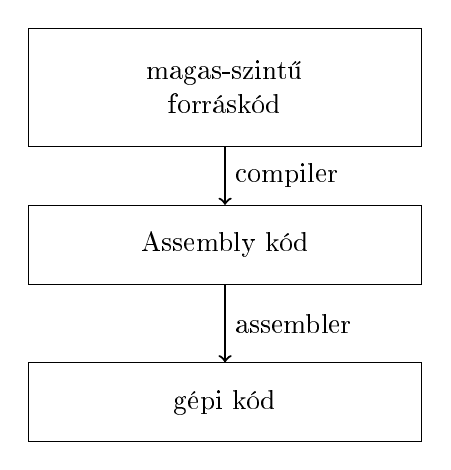
\begin{tikzpicture}
		% High-level source code
		\node[block, minimum width=5cm, minimum height=1.5cm] (highlevel) at (0,0) {};
		\node[align=center] at (highlevel) {magas-szintű\\forráskód};
		
		% Compiler
		\node[block, minimum width=5cm, minimum height=1cm] (compiler) at (0,-2.0) {};
		\node[align=center] at (compiler) {Assembly kód};
		
		% Assembly source code
		\node[block, minimum width=5cm, minimum height=1cm] (assembly) at (0,-4) {};
		\node[align=center] at (assembly) {gépi kód};
		
		% Arrows
		\draw[->, thick] (highlevel.south) -- (compiler.north) node[midway, right] {compiler};
		\draw[->, thick] (compiler.south) -- (assembly.north) node[midway, right] {assembler};
	\end{tikzpicture}
	\caption{A forráskód állapotának szakaszai}
\end{figure}

\newpage

\section{Adattárolás}

A számítógépen alapvetően háromféleképpen tárolhatjuk az adatainkat.

Léteznek a processzorban a \framebox{\textbf{regiszter}ek} , amik nagyon \textbf{gyorsak}, bár \textbf{kis méretű} adatok tárolására képesek. Ezt a kapacitást az adott architektúra határozza meg, így egy \textbf{32-bites processzoron 1 regiszter 32 bitet} (= 4 bájtot) tárol.\footnote{Vagy általánosan $n$-bites processzorban $n$-bitesek a regiszterek, ahol $n\in \mathbb{N}^+$ 2 hatványa.} Azon aktuális adatokat tároljuk el bennük, melyekkel \textbf{műveleteket akarunk végezni} (\textit{hatékonyan}).

A \framebox{\textbf{memória}} nevezhető az ``arany középútnak'', ugyanis \textbf{közepesen gyors} és \textbf{közepes a tárkapacitása}. Praktikus a programkód és a változók tárolására. A statikus memória, a \textbf{stack} és a \textbf{heap} is ezen helyezkedik el. A stack a program futásidejű, veremszerkezetű memóriája. A heapről sajnos nem lesz szó a tantárgy keretein belül.

És végül, de nem utolsó sorban, említésre méltóak a \framebox{\textbf{háttértárak}} . Ezek összehasonlítva \textbf{lassú}ak, cserébe \textbf{óriási tárkapacitás}sal rendelkeznek.

\subsection{Regiszterek}

32-bites architektúrán a regiszterek nevei \texttt{e}-vel kezdődnek.

\begin{figure}[h]
	\centering
	\begin{tabular}{|l|l|}
		\hline\hline
		\multicolumn{2}{|c|}{\textbf{Általános célú regiszterek}} \\
		\hline
		\makecell[l]{\texttt{eax}, \texttt{ebx}, \\ \texttt{ecx}, \texttt{edx}, \\ \texttt{esi}, \texttt{edi}} &  \makecell[l]{Egymással felcserélhetően használhatók (többnyire). \\
		Néhány \textit{konvenció}, ha C függvények hívásához használjuk őket. \\
		-- A függvény csak az \texttt{eax}, \texttt{ecx} és \texttt{edx} regisztereket hagyja \\
		~~ változatlanul, a többit ``elronthatja''. \\
		-- A visszatérési érték az \texttt{eax} regiszterbe kerül.
		}	\\
		\hline\hline
		\multicolumn{2}{|c|}{\textbf{Veremmel kapcsolatos regiszterek}} \\
		\hline
		\texttt{esp} & \textit{Stack pointe}r, a futási idejű verem tetejét mutatja. \\
		\hline
		\texttt{ebp} & \makecell[l]{\textit{Base pointer}, az éppen aktív eljáráshoz/függvényhez \\ tartozó adatokra mutat a veremben.} \\
		\hline\hline
		\multicolumn{2}{|c|}{\textbf{Egyéb regiszterek}} \\
		\hline
		\texttt{eip} & \textit{Instruction pointer}, a következő végrehajtandó utasításra mutat. \\
		\hline
		\texttt{eflags} & \makecell[l]{Jelzőbitek gyűjteménye, pl. ``az előző aritmetikai utasítás \\ eredménye nulla volt-e?''.} \\
		\hline
	\end{tabular}
	\caption{Regiszterek csoportosítása}
\end{figure}

Az \textit{egyéb regisztereket} \textbf{nem érjük el közvetlenül}, egyes utasítások olvassák/írják őket (pl. a \texttt{cmp} a \texttt{eflags}-et vagy a \texttt{call} a \texttt{eip}-t).

A regiszterek szerkezete a következő. Az általános célú regiszterek (pl. az \texttt{eax}, \texttt{ebx}, \texttt{ecx}, \texttt{edx}) feloszhatók alsóbb szeletekre, akár több szinten is. Így lesz egy 16-bites \texttt{ax} (a 0.-től a 15. bitig) és egy szintén 16-bites, ám név nélküli szelete (a 16.-tól a 31. bitjéig). Az \texttt{ax} tovább osztható \texttt{al}-re és \texttt{ah}-ra (8-8 bitesek, a \textit{low half} és \textit{high half} elnevezésből). Az \texttt{eax}, \texttt{ax}, \texttt{al} mind egy-egy regiszter, de \textbf{nem függetlenek egymástól}. Ugyanis ha az \texttt{al} megváltozik, akkor az \texttt{ax} és az \texttt{eax} is vele változik.

\begin{figure}[h]
	\centering
	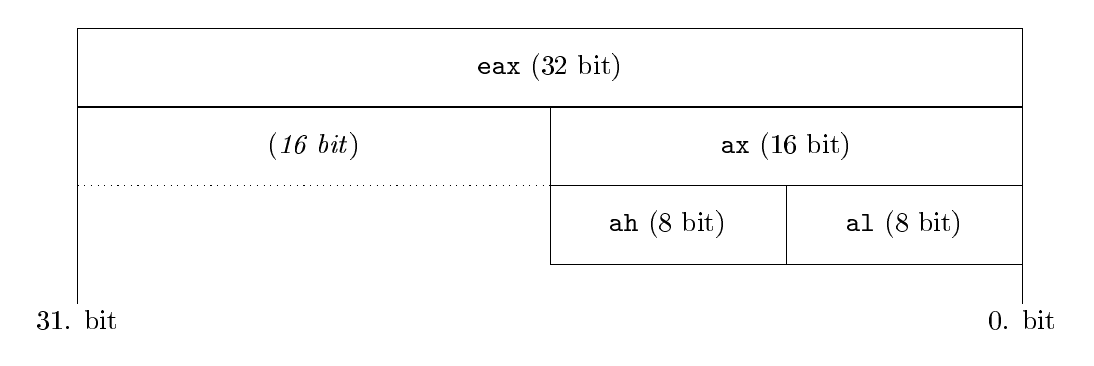
\begin{tikzpicture}
		\node[block, minimum width=12cm, minimum height=1cm] (eax) {\texttt{eax} (32 bit)};
		\node[block, minimum width=6cm, minimum height=1cm] at (3,-1) {\texttt{ax} (16 bit)};
		\node[selection, minimum width=6cm, minimum height=1cm] at (-3,-1) {(\textit{16 bit})};
		\node[block, minimum width=3cm, minimum height=1cm] at (4.5,-2) {\texttt{al} (8 bit)};
		\node[block, minimum width=3cm, minimum height=1cm] at (1.5,-2) {\texttt{ah} (8 bit)};
		
		\draw[-] (6, -3)  -- (6, 0) {};
		\draw[-] (-6, -3) -- (-6, 0) {};
		
		\node at (6, -3.2)  {0. bit};
		\node at (-6, -3.2) {31. bit};
	\end{tikzpicture}
	\caption{Az \texttt{eax}, \texttt{ebx}, \texttt{ecx}, \texttt{edx} szerkezete}
\end{figure}

Más regiszterek (\texttt{esp}, \texttt{esi}, \texttt{edi}, \texttt{ebp}, \texttt{eip}) is feloszhtatók ugyan kevesebb, de hasonlóan ``nevezetes szeletekre'', pl. \texttt{esp} (32-bit) -- \texttt{sp} (alsó 16 bit).

\begin{figure}[h]
	\centering
	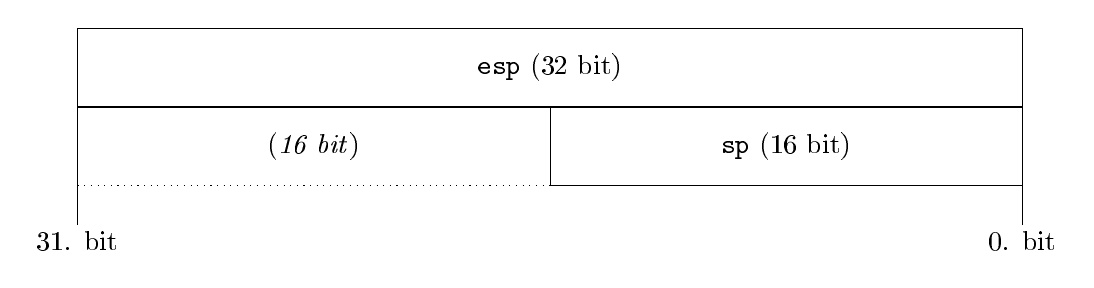
\begin{tikzpicture}
		\node[block, minimum width=12cm, minimum height=1cm] (esp) {\texttt{esp} (32 bit)};
		\node[block, minimum width=6cm, minimum height=1cm] at (3,-1) {\texttt{sp} (16 bit)};
		\node[selection, minimum width=6cm, minimum height=1cm] at (-3,-1) {(\textit{16 bit})};
		
		\draw[-] (6, -2)  -- (6, 0) {};
		\draw[-] (-6, -2) -- (-6, 0) {};
		
		\node at (6, -2.2)  {0. bit};
		\node at (-6, -2.2) {31. bit};
	\end{tikzpicture}
	\caption{Az \texttt{esp}, \texttt{esi}, \texttt{edi}, \texttt{ebp}, \texttt{eip} szerkezete}
\end{figure}


\subsection{Címkék}

A \textbf{címkék} arra szolgálnak, hogy az egyes memóriacímekre kényelmesebben tudjunk hivatkozni. Önmagában nem tárolnak sem típusinformációt, sem a változó méretét. Az utóbbiról kifejezetten fontos, hogy gondoskodjunk, ugyanis csak az alapján képes eldönteni a program, hogy az adott memóriacímtől kezdve hány bájtot olvasson be. Ha belegondolunk, ez hasonlít arra, ahogyan a C-ben a tömbök, pointerek működnek.

\begin{lstlisting}[style=asmstyle, caption={Assembly program. A forráskód kiterjesztése \texttt{*.asm}}]
global main		; global label used to denote the entry point of the program
extern <label>  ; label is declared but defined elsewhere (externally)

; uninitialised variables
section .bss
a: resd 1    ; 1x4 bytes reserved at 'a'
b: resw 1    ; 1x2 bytes reserved at 'b'
c: resb 256  ; 256x1 bytes reserved at 'c' (i.e. character array)

; initialised variables
section .data
d: dd 42      ; 1x4 bytes defined as '42' at 'd'
e: dw 1,2,3,4 ; 4x2 bytes defined as '1,2,3,4' at 'e' (array)
f: db 'a'     ; 1x1 bytes defined as 'a' (ASCII) at 'f'

; source code starts here
section .text
main:
	; machine instructions ...
\end{lstlisting}

\begin{itemize}
	\item \asmexample{global main} : Ebben a fájlban definiáljuk a ``main'' címkét, és szeretnénk, hogy globálisan látható
	legyen.
	\item \asmexample{extern <label>} : A \texttt{<label>} címke máshol van definiálva, de itt
	szeretnénk használni.
	\item \asmexample{section .bss} : Kezdőérték nélküli memóriaterület (``\textit{block starting symbol}''). \\
	A rövidítések jelentése: \texttt{res} $\longrightarrow$ ``\textit{reserve}''.
	\begin{flalign*}
		\texttt{res} \begin{cases}
			\texttt{b} \longrightarrow \text{``\textit{byte}''} & = 1 ~ \text{bájt}\\
			\texttt{w} \longrightarrow \text{``\textit{word}''} & = 2 ~ \text{bájt} \\
			\texttt{d} \longrightarrow \text{``\textit{double}''} & = 4 ~ \text{bájt}.
		\end{cases}
	\end{flalign*}
	\item \asmexample{section .data} : Kezdőértékkel rendelkező memóriaterület. \\
	A rövidítések jelentése: \texttt{d} $\longrightarrow$ ``\textit{define}''.
	\begin{flalign*}
		\texttt{d} \begin{cases}
			\texttt{b} \longrightarrow \text{``\textit{byte}''} & = 1 ~ \text{bájt}\\
			\texttt{w} \longrightarrow \text{``\textit{word}''} & = 2 ~ \text{bájt} \\
			\texttt{d} \longrightarrow \text{``\textit{double}''} & = 4 ~ \text{bájt}.
		\end{cases}
	\end{flalign*}
	\item \asmexample{section .text} : Itt kezdődik a programkód, az utasítások sorozata.
	\begin{itemize}
		\item Minden utasításnak lehet címkéje, de nem kötelező.
		Lehet csak címkét tartalmazó sor is.
		\item Önálló assembly programoknál a program belépési pontja a \texttt{\_start} címke,
		de megírhatjuk egy C program main függvényét is, ekkor \texttt{main} címkét
		használunk.
		\item Az utasításoknak van neve (mnemonikja) és operandusai.
		\item Megjegyzések: a \texttt{;} karaktertől a sor végéig.
	\end{itemize}
	\item \asmexample{main:} : Main címke; itt kezdődik a program ‘main’ függvénye.
\end{itemize}

A memóriahivatkozás címkékkel a következőképp történik:
\[ \texttt{<size> [<label>]}, \] ahol a \texttt{<size>} lehet \texttt{byte} (1 bájt), \texttt{word} (2 bájt) vagy \texttt{dword} (4 bájt), a \texttt{<label>} meg egy címke. Fontos, hogy ugyanolyan mérettel ``paraméterezzük fel'', amilyennek deklaráltuk.

A kódban az alábbi módon történne a memóriahivatkozás:
\[ \texttt{dword [a]}, ~~~~~ \texttt{word [b]}, ~~~~~ \texttt{byte [c]} ~~ \text{(a tömb első eleme)}. \]
A hivatkozásba írhatók regiszterekből, címkékből és számliterálokból álló egyes kifejezések, pl.:
\[ \texttt{dword [a+4*ecx]} ~~ \text{(az \texttt{a} tömb 4. eleme, ha 4 bájtosak az egyes elemek)}. \]

\pagebreak

\section{Utasítások, műveletek}

Először általánosságokban beszélünk az Assembly utasításairól, utána csoportonként átnézzük a specifikusabb részleteket.

Ahogy azt megfigyelhettük, az Assembly utasításai \textbf{prefix jelölés}t használnak. Ez jó, mert a fordítók hatékonyan fel tudják dolgozni (lásd \textit{Algoritmusok és adatszerkezetek I.}). Egy utasítás felvehet 0, 1 vagy 2 paramétert.

A kétparaméteres utasítások szerkezete a következő:
\[ \texttt{instruction <destination> <source>}. \]

Értelemszerűen az \texttt{instruction} jelöli az utasítást. A \texttt{<destination>} lehet regiszter vagy memóriahivatkozás, míg a \texttt{<source>} lehet regiszter, memóriahivatkozás vagy literál. 

\textbf{Legfeljebb az egyik lehet memóriahivatkozás!}

Továbbá biztosítanunk kell a megfelelő \textbf{offset}et, azaz \textbf{memóriahivatkozásnál meg kell adnunk az olvasandó méretet }a fent bemutatott módon (\texttt{byte}, \texttt{word}, \texttt{dword}). Ha valamelyik operandus regiszter, akkor abból kiderül, így elhagyható.

A művelet \textbf{végeredménye a \texttt{<destination>} által jelölt memóriacímbe lesz írva}.

\begin{lstlisting}[style=asmstyle, caption={Helyes paraméterezés}]
; correct
mov eax,0   ; one of them is a register, the size is evident
mov bx,ax   ; the sizes of the two registers are equal
mov [lab1], al ; one of them is a register, the size is evident
mov dword [lab2], 987 ; the size of the label needs to be specified
mov ebx, [lab3] ; one of them is a register, the size is evident
\end{lstlisting}

\begin{lstlisting}[style=asmstyle, caption={Helytelen paraméterezés}]
; incorrect
mov byte [lab4], byte [lab5] ; two labels are not allowed
mov al, ax ; the sizes of the two registers are NOT the same
\end{lstlisting}

Egyparaméteres utasításoknál a végeredmény az egyetlen paraméter memóriacímében lesz elhelyezve:
\[ \texttt{instruction <parameter>}. \]
A \texttt{<parameter>} operandus lehet regiszter vagy memóriahivatkozás.

\subsection{Adatmozgató utasítások}

Utasítás: \texttt{mov}. A mozgatás valójában másolást jelent: a ``honnan'' nem változik meg.

\subsection{Aritmetikai utasítások}

Kétparaméteres műveletek: \texttt{add} (összeadás), \texttt{sub} (kivonás).

Egyparaméteres műveletek: \texttt{inc} (inkrementálás), \texttt{dec} (dekrementálás).

A szorzás (\texttt{mul}) és osztás (\texttt{div}) igs egyparaméteres műveletek, azonban a működésük nem teljesen intuitív.

A szorzás összeszorzza az \texttt{eax} és a paraméterül kapott memóriacím tartalmát. Az eredmény az \texttt{eax}-be kerül, azonban túlcsoldulás esetén a további bitek az \texttt{edx}-ben lesznek rögzítve.

\begin{lstlisting}[style=asmstyle]
mov eax, 5      ; Load 5 into eax
mov ebx, 6      ; Load 6 into ebx
mul ebx         ; Multiply eax by ebx (5 * 6 = 30)
; After this, eax = 30 and edx = 0 because the result fits in 32 bits
\end{lstlisting}

A \texttt{div} is hasonló elvet követ -- ott csupán nem a túlcsordulás esete áll fenn, hanem az osztási maradéké. Ez az, amit az \texttt{edx}-ben eltárol.

\begin{lstlisting}[style=asmstyle]
mov eax, 30     ; Load 30 into eax
mov edx, 0      ; Clear edx
mov ecx, 4      ; Load 4 into ecx
div ecx         ; Divide edx:eax by ecx (30 / 4)
; After this, eax = 7 (quotient), edx = 2 (remainder)
\end{lstlisting}

\textbf{\textit{Megjegyzés}}. Felhívjuk a figyelmet, hogy a \texttt{mul} és \texttt{div} előjel nélküli egész számoknak tekinti az operandusait. Előjeles számok esetén \texttt{imul} és \texttt{idiv} használandó.

\subsection{Bitműveletek}

Kétparaméteres műveletek: \texttt{and}, \texttt{or}, \texttt{xor}.

Egyparaméteres műveletek: \texttt{not}.

\subsection{Ugróutasítások}

Módosíthatják azon regiszterek tartalmát (\texttt{eip}\footnote{A következő végrehajtandó utasításra mutat.}, \texttt{eflags}\footnote{Jelzőbitek gyűjteménye, pl. ``az előző aritmetikai utasítás eredménye nulla volt-e?''.}), amihez amúgy nincs közvetlen hozzáférésünk.

\subsubsection{Feltétel nélküli ugrás}

Egyparaméteres utasítások: \texttt{jmp <label>}.\footnote{Megfeleltethető ``\textit{az átkos}'' \texttt{goto} utasításnak.} Módosítja az \texttt{eip}-t.%Általában címkékkel szoktuk felparaméterezni.

// Ábra

\subsubsection{Feltételes ugrások}

Kétparaméteres utasítások: \texttt{cmp <mit> <mivel>} (\textit{compare}).
\begin{enumerate}
	\item A \texttt{cmp} utasítás kivonást végez, de nem tárolja el az eredményt, hanem annak előjele alapján jelzőbiteket állít át az \texttt{eflags} regiszterben.
	\item Ha a kivonás eredménye 0 (azaz az összehasonlított értékek egyenlők), akkor a \textbf{zero flag} 1 lesz, különben 0.
\end{enumerate}

Egyparaméteres utasítások: \texttt{je} (\textit{jump if equal}), \texttt{jne} (\textit{jump if not equal}), \texttt{jb} (\textit{below}) = \texttt{jnae}, \texttt{ja} (\textit{above}) = \texttt{jnbe}, \texttt{jnb} = \texttt{jae}, \texttt{jna} = \texttt{jbe}. 
\begin{enumerate}
	\item A feltételes ugró utasítások a jelzőbiteket figyelik.
	\item A \texttt{je} akkor ugrik, ha a \textbf{zero flag} 1, egyébként a következő utasításra kerül a vezérlés.
\end{enumerate}

\textbf{\textit{Megjegyzés}}. Ezek előjel nélküli egész számokat feltételeznek!

// Ábra

\subsubsection{Feltételes adatmozgatás}

Kétparaméteres utasítások: \texttt{cmov <hova> <honnan>} (\textit{conditional move}).

// Ábra

\subsubsection{Elágazások, ciklusok}

\begin{figure}[h]
	\centering
	\begin{minipage}{0.25\linewidth}
		\begin{lstlisting}[style=asmstyle, caption={Egyágú elágazás}]
cmp eax,ebx
je egyenlo
mov eax,ebx
egyenlo:
		\end{lstlisting}
	\end{minipage}
\begin{minipage}{0.05\linewidth}
	~
\end{minipage}
\begin{minipage}{0.25\linewidth}
	\begin{lstlisting}[style=asmstyle, caption={Kétágú elágazás}]
cmp ebx,ecx
ja nagyobb
mov eax,ecx
jmp vege
nagyobb:
mov eax,ebx
vege:
	\end{lstlisting}
\end{minipage}
\begin{minipage}{0.05\linewidth}
	~
\end{minipage}
\begin{minipage}{0.25\linewidth}
	\begin{lstlisting}[style=asmstyle, caption={Ciklus}]
mov eax,0
eleje: cmp ecx,0
je vege
add eax,ecx
dec ecx
jmp eleje
vege:
	\end{lstlisting}
\end{minipage}
\end{figure}

\subsection{Veremműveletek}

Minden futó programhoz tartozik egy verem vagy más néven \textbf{stack}. Ezt a memóriaterületet az \textbf{operációs rendszer rendeli hozzá} a programhoz. Az \asmexample{esp} regiszter mutatja a verem tetejét. Általában itt tároljuk:
\begin{itemize}
	\item függvények paraméterei
	\item függvények visszatérési címe
	\item függvények lokális változói
	\item időlegesen tárolt adatok
\end{itemize}

Nem meglepően, a kapcsolódó \textit{egyparaméteres műveletei}: \texttt{push} és \texttt{pop}.

\textbf{\textit{Megjegyzés}}. Mindkét esetben csak 2 vagy 4 bájtos lehet az operandusa a két utasításnak!

// Ábra

\subsubsection{Függvényhívás és visszatérés}

Egyparaméteres utasítás: \texttt{call <címke>}. Valójában ez is egyfajta ugróutasítás.

Paraméter nélküli utasítás: \texttt{ret}.

\textbf{\textit{Megjegyzés}}. Mindkettő módosítja az \texttt{eip} és az \texttt{esp} értékét!

// Ábra

\subsubsection{Függvényhívás paraméterrel}

Nincsenek külön műveletek erre -- az idáig bemutatottakat alkalmazzuk.
\begin{itemize}
	\item A függvény paraméterét a
	verembe tesszük a hívás
	előtt.
	\item A függvény törzse
	kimásolja a paramétert a
	veremből.
	\item A visszatérési érték az
	\texttt{eax} regiszterben van.
	\item A hívás után kivesszük a
	paramétert (vagy legalább
	a veremmutatót
	visszaállítjuk).
\end{itemize}

%\newpage

\section{Fordítás}

A fordításhoz a \texttt{nasm} assemblert használjuk, ami előállítja a \textbf{tárgykódot}.

Vegyük az alábbi kódokat!

\begin{figure}[h]
\begin{minipage}{0.45\linewidth}
	\begin{lstlisting}[style=asmstyle, caption={\texttt{addone.asm}}]
global main
extern write_natural
extern read_natural

section .text
main:
call read_natural
inc eax
push eax
call write_natural
add esp,4
mov eax,0
ret
	\end{lstlisting}
\end{minipage}
\begin{minipage}{0.05\linewidth}
	~
\end{minipage}
\begin{minipage}{0.45\linewidth}
	\begin{lstlisting}[style=cppstyle, caption={\texttt{io.c}}]
#include <stdio.h>

void write_natural(unsigned n) 
{
	printf("%u\n", n);
}

unsigned read_natural() 
{
	unsigned ret;
	scanf("%u", &ret);
	return ret;
}
	\end{lstlisting}
\end{minipage}
\end{figure}

Az \texttt{addone.asm} meghívja az \texttt{io.c}-ből a \texttt{read\_natural} függvényt, ami beolvas egy előjel nélküli természetes számot, majd ezt kiíratja a \texttt{write\_natural} meghívásával. Végül a program terminál.

Az említett két függvényt az egyszerűség kedvéért C-ben írjuk meg.
Lehetne tisztán Assemblyben is, de az jóval bonyolultabb volna.

Első lépésként az Assembly kódot fordítjuk le. A \texttt{-felf} kapcsolóval megadjuk a fájl formátumát (a mi esetünkben ez \texttt{elf}).

\begin{lstlisting}[style=machinestyle]
nasm -felf addone.asm
\end{lstlisting}

Ezután a C fordítóval lefordítjuk gépi kódra az \texttt{io.c}-t, majd összelinkeljük a kapott tárgykódokat, ügyelve arra, hogy 32-bites architektúrájúra fordítsuk le (\texttt{-m32}).

\begin{lstlisting}[style=machinestyle]
gcc -m32 -oaddone io.c addone.o
\end{lstlisting}

Végül nincs más hátra, mint hogy kipróbáljuk!

\begin{lstlisting}[style=machinestyle]
./addone
41
42
\end{lstlisting}
\chapter{Kódgenerálás}

Elérkeztünk a kurzus azon pontjára, amikor is megkoronázzuk az eddigi munkálatainkat, azaz a fordítóprogramunk működő számítógépes programot képes gyártani!

\section{Kódgenerálás attribútumnyelvtannal}

Kódot generálni általában úgy szoktunk, hogy \textbf{transzlációval} a saját, magas szintű nyelvünket lefordítjuk \textbf{Assemblyre}, majd az assembler legenerálja nekünk a kívánt gépi kódot. Kizárólag indokolt esetben érdemes közvetlenül gépi kódot generálni.

Ott hagytuk abba, hogy a szemantikus elemző ellenőrizte a deklarációkat a szimbólumtáblával és a típusokat az attribútumnyelvtannal. Haladjunk ezen az útvonalon -- pontosabban az alulról felfele, $LR$ elemző megoldásának útján.

A szabályok bal oldalaihoz, mint láttuk, felvettünk attribútumokat, melyek különféle tulajdonságokat határoztak meg. \textit{Miért ne tehetnénk meg ugyanezt magával a kód generálásával}?

\textbf{Vegyük fel} a \textit{szabályok bal oldalához} a \textbf{következő szintetizált attribútumot}: $code : \mathbb{S}$. Ez egy egyszerű sztring lesz, amihez hozzákonkatenáljuk az egyes részeket, ahogy haladunk felfele a szintaxisfában.

A nyelvtan továbbra is \[\prodrule{E}{\texttt{int\_literal} \mid \texttt{identifier} \mid E ~ \texttt{less\_than} ~ E}.\]

A mondatunk: \[ \texttt{10 < x}. \]

Az elemzett szintaxisfa eddigi állapota:

\begin{figure}[h]
	\centering
	\begin{forest}
		for tree={edge={-}, l sep-=10pt, s sep+=10pt}
		[$E$\textsuperscript{$type : \text{bool}$}
		[$E$\textsuperscript{$type : \text{int}$}
		[\texttt{int\_literal}\textsuperscript{$value : 10$}, tier=terminal]
		]
		[\texttt{less\_than}, tier=terminal]
		[$E$\textsuperscript{$type : \text{int}$}
		[\texttt{identifier}\textsuperscript{$name : \texttt{x}$}, tier=terminal]
		]
		]
	\end{forest}
\end{figure}

A korábban definiált, szabályokhoz rendelt \textbf{akciókat módosítsuk} úgy, hogy megadjuk az Assembly kódrészleteket.

\begin{stuki*}[14cm]{$\prodrule{E}{\texttt{int\_literal}}$}
	\stm{E.type := \text{int}}
	\stm{E.code := "\texttt{mov eax ,}" + \texttt{int\_literal}.value +"\texttt{\textbackslash n}"}
\end{stuki*}

\begin{stuki*}[14cm]{$\prodrule{E}{\texttt{identifier}}$}
	%\stm{\text{/* Ellenőrzés: Deklarálva volt-e az azonosító? */}}
	\begin{IF}[20]{5}{\stm{\texttt{identifier}.name \notin symbol\_table}}
		\stm{error(\dots)}
		\ELSE
		\stm{type := symbol\_table.get\_type(\texttt{identifier}.name)}
		\stm{E.type := type}
		\begin{CASE}{2}{2}
			\WHEN{\stm{E.type = \text{int}}}
			\stm[2]{E.code := \\ "\texttt{mov eax, [}" + type + "\texttt{]\textbackslash n}"}
			\WHEN{\stm{\dots}}
			\stm{\text{/* Ha logikai lenne, az} \\ \text{kisebb regiszterben is elférne */}}
		\end{CASE}
	\end{IF}
\end{stuki*}

\begin{stuki*}[14cm]{$\prodrule{E_1}{E_2 ~ \texttt{less\_than} ~ E_3}$}
	%\stm{\text{/* Ellenőrzés: Megfelelő típusúak-e a ``\texttt{<}'' operátor paraméterei? */}}
	\begin{IF}[20]{4}{\stm{E_2.type \neq \text{int} \lor E_3.type \neq \text{int}}}
		\stm{error(\dots)}
		\ELSE
		\stm{E_1.type := \text{bool}}
		\stm[3]{E_1.code :=  E_2.code + "\texttt{push eax\textbackslash n}" + \\ E_3.code + "\texttt{mov ebx, eax\textbackslash n}" + "\texttt{pop eax \NEWLINE}" + \\ "\texttt{cmp eax, ebx\NEWLINE}" + "\texttt{mov al, 0\NEWLINE}" + "\texttt{cmovb al, 1\NEWLINE}"}
	\end{IF}
\end{stuki*}

Ahhoz, hogy megkönnyítsük a munkánkat, bevetejünk ún. kódgenerálási sémákat, melyek hatékonyabbá teszik az Assembly kódok ``megkomponálását''.

\section{Kódgenerálási sémák}

A sémákat nem szabványos struktogramok formájában írom fel.

A számokat 32 bites, előjeles egész számként fogjuk tárolni. Minden szám típusú kifejezés eredményét az \texttt{eax} regiszterbe fogjuk kiszámolni.

\begin{figure}[h]
	\begin{stuki*}[5cm]{$\prodrule{E}{\texttt{int\_literal}}$}
		\stm*{\texttt{mov eax,} \textit{literál értéke}}
	\end{stuki*}
	\caption{Számliterál kifejezés kódgenerálási sémája}
\end{figure}

A logikai értékeket 1 bájton fogjuk tárolni. Adatreprezentáció: $false = 0$ és $true = 1$. Minden logikai típusú kifejezés eredményét az \texttt{al} regiszterbe fogjuk kiszámolni.

\begin{figure}[h]
	\begin{minipage}{0.5\linewidth}
		\begin{stuki*}[5cm]{$\prodrule{E}{\texttt{false}}$}
			\stm*{\texttt{mov al, 0}}
		\end{stuki*}
	\end{minipage}
	\begin{minipage}{0.5\linewidth}
		\begin{stuki*}[5cm]{$\prodrule{E}{\texttt{true}}$}
			\stm*{\texttt{mov al, 1}}
		\end{stuki*}
	\end{minipage}
	\caption{Logikai literál kifejezés kódgenerálási sémája}
\end{figure}

A változók adatait a szimbólumtáblában tároljuk. Mindegyikhez egy egyedi címkét generálunk, amikor betesszük őket a táblába. A változó használatakor kiolvassuk a címkét, és beépítjük a generált kódba.

\begin{figure}[h]
	\begin{minipage}{0.5\linewidth}
		\begin{stuki*}[5cm]{$\prodrule{E}{\texttt{identifier}}$}
			\stm*{\texttt{mov eax,} \texttt{[}\textit{címke}\texttt{]}}
		\end{stuki*}
	\end{minipage}
	\begin{minipage}{0.5\linewidth}
		\begin{stuki*}[5cm]{$\prodrule{E}{\texttt{identifier}}$}
			\stm*{\texttt{mov al,} \texttt{[}\textit{címke}\texttt{]}}
		\end{stuki*}
	\end{minipage}
	\caption{Változó mint kifejezés kódgenerálási sémája}
\end{figure}

Ehhez megtesszük az értelemszerű módosításokat a szimbólumtábla implementációjában is.

\begin{figure}[h]
	\centering
	
	\struct{SymbolTable}
	+ $name : \mathbb{S}$ \\
	\vdots \\
	%+ $kind : Kind$ \\
	%+ $type : Type$ \\
	%+ $declaration : \mathbb{N} \times \mathbb{N}$ ~ \texttt{/* (row, column) */} \\
	%+ $used\_here : \mathbb{N} \times \mathbb{N}\langle\rangle$ \texttt{/* list of coordinates */}\\
	+ $code : \mathbb{S}$ \\
	+ $label : \mathbb{S}$ \\
	\hline
	+ SymbolTable(\dots) \\
	\vdots \\
	+ \underline{next\_label$():\mathbb{S}$} \\ 
	\texttt{/* additional methods may come here */} \\
	\eoStruct
	\caption{A szimbólumtábla egy lehetséges módosítása}
\end{figure}

Beépített operátorok kódgenerálási sémája:

\begin{figure}[h]
	\begin{minipage}{0.5\linewidth}
		\begin{stuki*}[5cm]{$\prodrule{E_1}{E_2 \texttt{ plus\_op } E_3}$}
			\stm*[6]{
				\textit{$E_2$ kódja} \\
				\texttt{push eax} \\
				\textit{$E_3$ kódja} \\
				\texttt{mov ecx, eax} \\
				\texttt{pop eax} \\
				\texttt{add eax, ecx}}
		\end{stuki*}
	\end{minipage}
	\begin{minipage}{0.5\linewidth}
		\begin{stuki*}[5cm]{$\prodrule{E}{\texttt{identifier}}$}
			\stm*[6]{
				\textit{$E_2$ kódja} \\
				\texttt{push eax} \\
				\textit{$E_3$ kódja} \\
				\texttt{mov ecx, eax} \\
				\texttt{pop eax} \\
				\texttt{mul eax, ecx}}
		\end{stuki*}
	\end{minipage}
	\caption{Összeadás és szorzás kódgenerálási sémája}
\end{figure}

\begin{figure}[h]
	\begin{minipage}{0.5\linewidth}
		\begin{stuki*}[5cm]{$\prodrule{E_1}{E_2 \texttt{ plus\_op } E_3}$}
			\stm*[7]{
				\textit{$E_2$ kódja} \\
				\texttt{push eax} \\
				\textit{$E_3$ kódja} \\
				\texttt{mov ecx, eax} \\
				\texttt{pop eax} \\
				\texttt{cmp eax, ecx} \\
				\texttt{mov al, 0} \\
				\texttt{cmovb al, 1}}
		\end{stuki*}
	\end{minipage}
	\begin{minipage}{0.5\linewidth}
		\begin{stuki*}[5cm]{$\prodrule{E}{\texttt{identifier}}$}
			\stm*[6]{
				\textit{$E_2$ kódja} \\
				\texttt{push ax} \\
				\textit{$E_3$ kódja} \\
				\texttt{mov cx, ax} \\
				\texttt{pop ax} \\
				\texttt{and al, cl}}
		\end{stuki*}
	\end{minipage}
	\caption{Kisebb operátor és logikai ``és'' kódgenerálási sémája}
\end{figure}

\pagebreak

Értékadás kódgenerálási sémája egész számra (bal oldal) és logikai értékre (jobb oldal). A változó címkéjét itt is a szimbólumtáblából vesszük.

\begin{figure}[h]
	\begin{minipage}{0.5\linewidth}
		\begin{stuki*}[5cm]{$\prodrule{U}{ \texttt{identifier} ~ \texttt{assign\_op} ~ E}$}
			\stm*[2]{
				\textit{E kódja} \\
				\texttt{mov [\textit{címke}], eax}}
		\end{stuki*}
	\end{minipage}
	\begin{minipage}{0.5\linewidth}
		\begin{stuki*}[5cm]{$\prodrule{U}{ \texttt{identifier} ~ \texttt{assign\_op} ~ E}$}
			\stm*[2]{
				\textit{E kódja} \\
				\texttt{mov [\textit{címke}], al}}
		\end{stuki*}
	\end{minipage}
	\caption{Értékadás kódgenerálási sémája}
\end{figure}

Elágazás kódgenerálási sémái. A kódgenerálási sémában szereplő címkék (pl. \textit{vége},
\textit{hamis}) helyett a séma minden felhasználásakor egyedi címkéket kell generálni (pl. \texttt{label0}, \texttt{label1}, \texttt{label2}, \dots)\footnote{Lásd a módosított UML-diagramot.}

\begin{figure}[h]
	\begin{minipage}{0.5\linewidth}
		\begin{stuki*}[5cm]{$\prodrule{U}{ \texttt{if} ~ E ~ \texttt{then} ~ P ~ \texttt{end}}$}
			\stm*[5]{
				\textit{E kódja} \\
				\texttt{cmp al, 1} \\
				\texttt{jne near \textit{vége}} \\
				\textit{P kódja} \\
				\texttt{\textit{vége}:}}
		\end{stuki*}
	\end{minipage}
	\begin{minipage}{0.5\linewidth}
		\begin{stuki*}[5cm]{$\prodrule{U}{ \texttt{if} ~ E ~ \texttt{then} ~ P_1 ~ \texttt{else} ~ P_2 ~ \texttt{end}}$}
			\stm*[7]{
				\textit{E kódja} \\
				\texttt{cmp al, 1} \\
				\texttt{jne near \textit{hamis}} \\
				\textit{$P_1$ kódja} \\
				\texttt{jmp \textit{vége}} \\
				\texttt{hamis:} \\
				\textit{$P_2$ kódja}
				\texttt{\textit{vége}:}}
		\end{stuki*}
	\end{minipage}
	\caption{Egy- és kétágú elágazás kódgenerálási sémája}
\end{figure}

\begin{figure}[h]
	\begin{minipage}{0.5\linewidth}
		\begin{stuki*}[5cm]{$\prodrule{U}{ \texttt{while} ~ E ~ \texttt{do} ~ P ~ \texttt{done}}$}
			\stm*[7]{
				\texttt{\textit{eleje}:} \\
				\textit{E kódja} \\
				\texttt{cmp al, 1} \\
				\texttt{jne near \textit{vége}} \\
				\textit{P kódja} \\
				\texttt{jmp \textit{eleje}} \\
				\texttt{\textit{vége}:}}
		\end{stuki*}
	\end{minipage}
	\begin{minipage}{0.5\linewidth}
		\begin{stuki*}[5cm]{$\prodrule{U}{ \texttt{do} ~ P ~ \texttt{while} ~ E}$}
			\stm*[5]{
				\texttt{\textit{eleje}:} \\
				\textit{P kódja} \\
				\textit{E kódja} \\
				\texttt{cmp al, 1} \\
				\texttt{je near \textit{eleje}}}
		\end{stuki*}
	\end{minipage}
	\caption{Elöl- és hátultesztelő ciklus kódgenerálási sémája}
\end{figure}

\pagebreak

Utolsó előtti lépésként a \textbf{szimbólumtáblát is rögzítenünk kell a kódban}. Ehhez végigiterálunk a tábla bejegyzésein és az \textbf{Assembly kód \texttt{.bss} szekciójába} beillesztjük. Sem a név, sem a méret miatt nem kell aggódnunk, ugyanis ezek az információk mind kinyerhetők a $label:\mathbb{S}$ (változónév) és $type:\text{Type}$ (méret) attribútumok segítségével.

\begin{figure}[h]
	\centering
	\begin{minipage}{0.5\linewidth}
		\begin{tabular}{|c|c|c|c|}
			\hline
			\textbf{Név} & \textbf{Fajta} & \textbf{Típus} & \textbf{Címke} \\
			\hline\hline
			\texttt{b} & változó & bool & \textit{lab0} \\
			\hline
			\texttt{i} & változó & int & \textit{lab1} \\
			\hline
		\end{tabular}
	\end{minipage}
	\begin{minipage}{0.3\linewidth}
		\begin{lstlisting}[style=asmstyle]
section .bss
lab0: resb 1
lab1: resd 1
		\end{lstlisting}
	\end{minipage}
\end{figure}

Végül, a teljes program sémája. Ebbe fognak beillesztődni az egyes kódsémák, kódrészletek, amint az elemző elérte a szintaxisfa gyökerét.

\begin{lstlisting}[style=asmstyle, caption={A teljes program sémája}]
global main
extern ; external labels

section .bss
; variables from symbol table

section .text
main:
; program instructions
ret
\end{lstlisting}
%\chapter{Fordítóprogramok}
%\chapter{Fordítóprogramok}

\backmatter
% bibliography, glossary and index would go here.

\end{document}